
Purely hadronic events originating from QCD interactions in proton-proton collisions account for the vast majority of events observed at the LHC. Not surprisingly, these events are a major background to new physics signals that may manifest in the hadronic channel. Several features of multi-jet QCD events are poorly modeled, including the production cross section, jet multiplicity, and relationships between the directions of jets. This motivates the development of data-driven approaches to QCD estimation. Typically, one takes advantage of the particularly well-modeled aspects of event simulation, but relies on the real data to model as many features as possible. As with any data-driven approach the method must be robust against possible signal contamination that may enter into control regions. 

\subsection{The origin of $\met$ in QCD events}
In order to estimate the QCD background contribution in signal regions with large $\met$, it is helpful to make use of the knowledge that the only stable particles in the $\SM$ that are invisible to the CMS detector are neutrinos. Apart from rare final states containing heavy-flavor jets,  QCD events are free of neutrinos, and therefore exhibit little or no $\met$ at the parton level.  For this reason, the $\met$ typically serves as an excellent discriminating variable between the large QCD background and events with significant $\met$, such as models of $R$-parity conserving supersymmetry (see Chapter \ref{chap:susy}). However, QCD events {\it only} exhibit zero $\met$ at the parton level $(\met)_{\rm part}$. The final-state particles are detected by a tracker and calorimeters with finite momentum and energy resolution. Mis-measurements of the jet momenta propagate into the measured missing transverse energy, inducing a sometimes significant missing transverse energy measurement $(\met)_{\rm meas}$, resulting in the QCD events occupying a similar kinematic region as events predicted by models of new physics.  These statements can be summarized as follows:
\begin{align}
%\begin{split}
(\vec{E}_{ T}^{\rm miss})_{\rm part} &\equiv -\sum_{i=1}^{n}(\vec{p}_{T})_{i,\rm part\ }=0\\
(\vec{E}_{ T}^{\rm miss})_{\rm meas} &\equiv -\sum_{i=1}^{n}(\vec{p}_{T})_{i,\rm meas\ \ \ }\neq 0,
%\end{split}
\label{eq:metTrue}
\end{align}
where $i$ is the particle index and $n$ is the number of particles in the event.

\subsection{Model assumptions and likelihood} 
In general, the magnitudes of the four-vectors of jets at the parton and reconstruction levels differ. However, assuming their directions are identical, the following expression holds for the collection of jets of a given event,
\begin{equation}
\vec{J}_{\rm meas} = \hat{C} \vec{J}_{\rm part},
\end{equation}
where $\vec{J}_{\rm meas}$ and $\vec{J}_{\rm part}$ are $n\times 1$ vectors of the reconstructed jet four-vectors and the parton-level jet four-vectors, and $\hat{C}$ is diagonal $n\times n$ matrix whose elements are the jet energy scale factors $(c_1,c_2,...,c_n)$. The likelihood for a scale factor $c_i\equiv p^{\mu}_{i,\rm meas}/p^{\mu}_{i,\rm part}$, given by
\begin{equation}
L_{i}\equiv{\rm P}(p^{\mu}_{i,\rm meas}|\ p^{\mu}_{i,\rm part})={\rm P}(c_i\ |\ p^{\mu}_{i,\rm part}),
\label{eq:JetEnergyLikelihood}
\end{equation}
is derived from simulation as the distribution of the ratio of reconstruction-level jet momentum to the associated parton-level jet momentum. The association of parton- and reconstruction-level jets is accomplished through the matching criterion,
\begin{equation}
\Delta R(p^{\mu}_{\textrm meas},p^{\mu}_{\textrm parton})<0.4.
\end{equation}	
Additionally, an isolation criterion,
\begin{equation}
p_{\rm T}/\sum_{i=1}^{\njets}[(p_{\rm T})_{i}\cdot\Theta(0.5-\Delta R(p^{\mu}_{i},p^{\mu}))]<1.01,
\end{equation}
is applied both to the parton-level jets and to the reconstruction-level jets that contribute to the likelihood. The likelihood, as shown in Figure \ref{fig:SmearEx}, is derived in bins of parton-level jet $p_T$ and $\eta$.
\begin{figure}[h]
\centering
\subfloat[]{
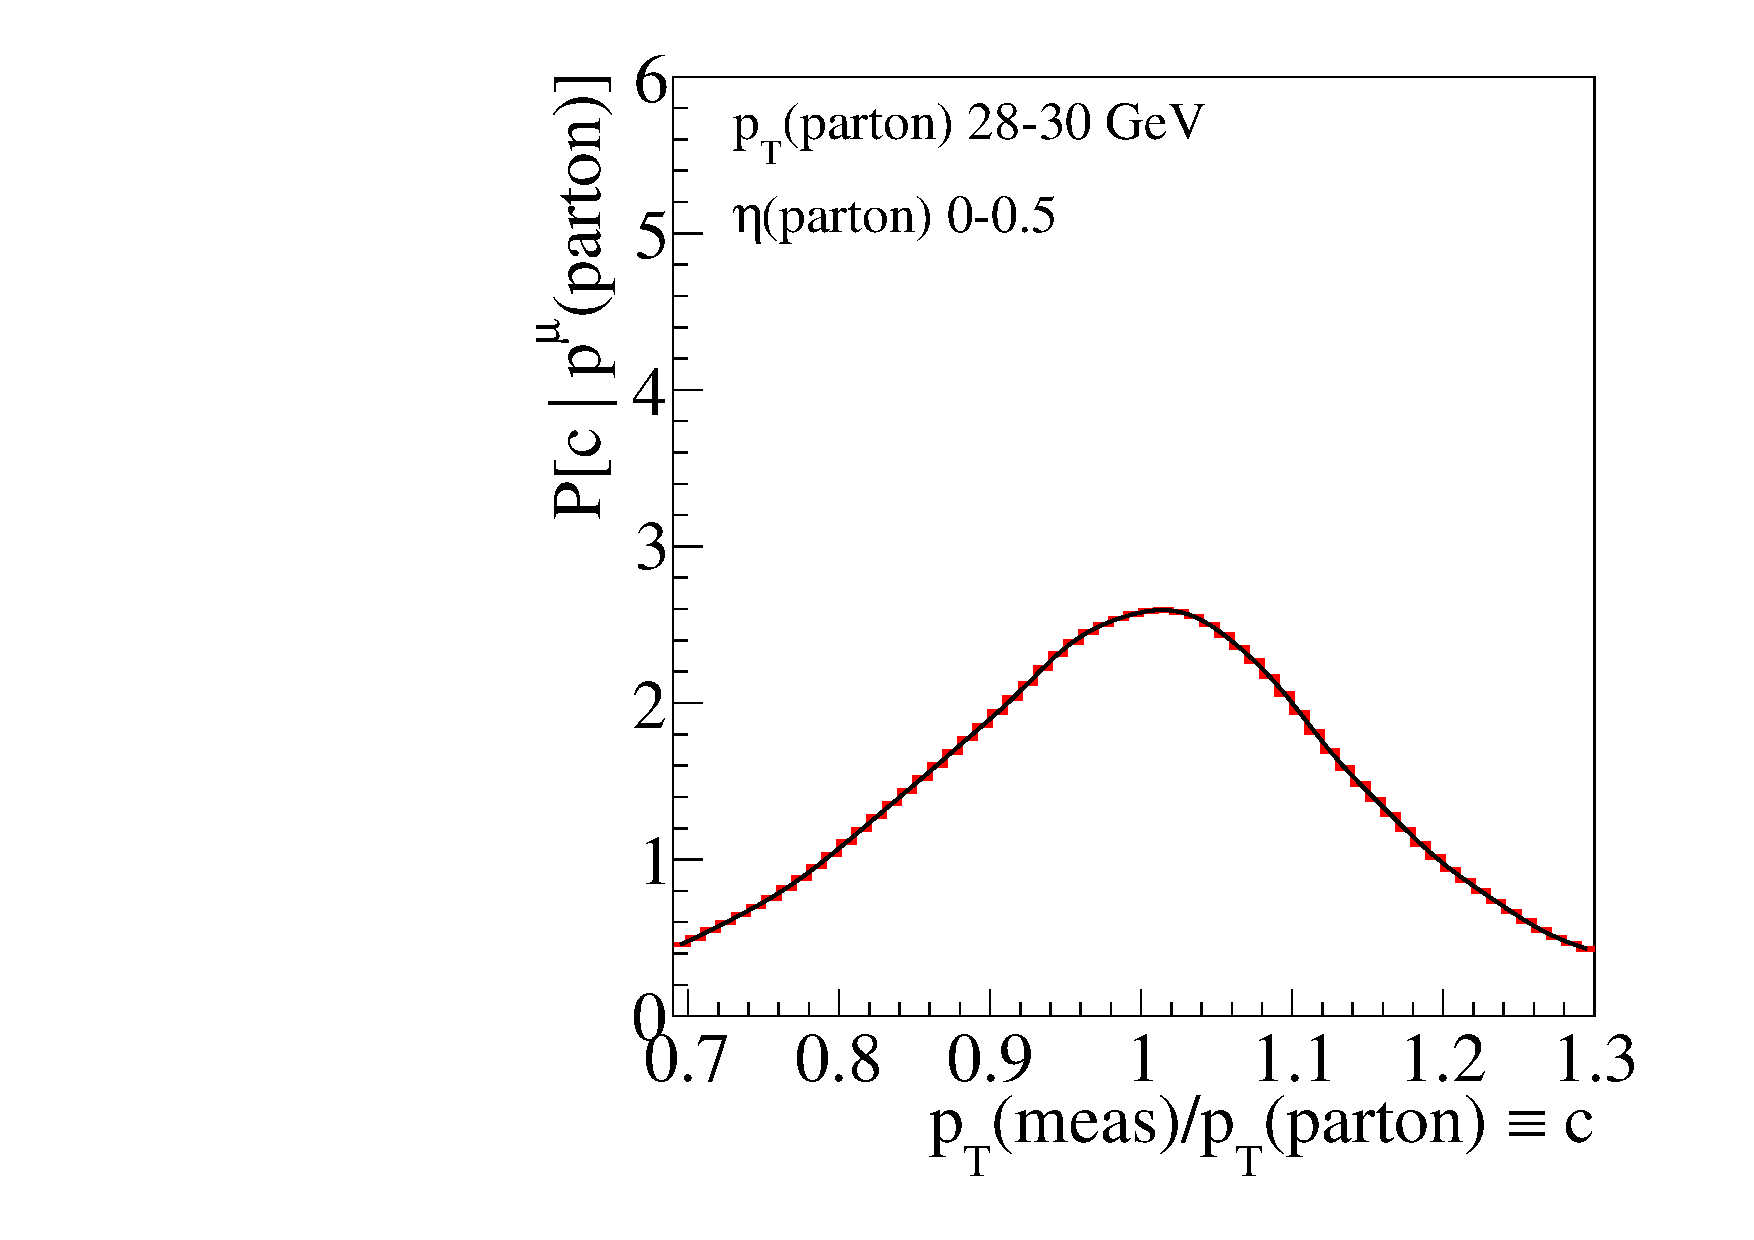
\includegraphics[width=0.5\linewidth]{figures/SusySearches/Ra2b2016/SmearEx1.pdf}
}
\subfloat[]{
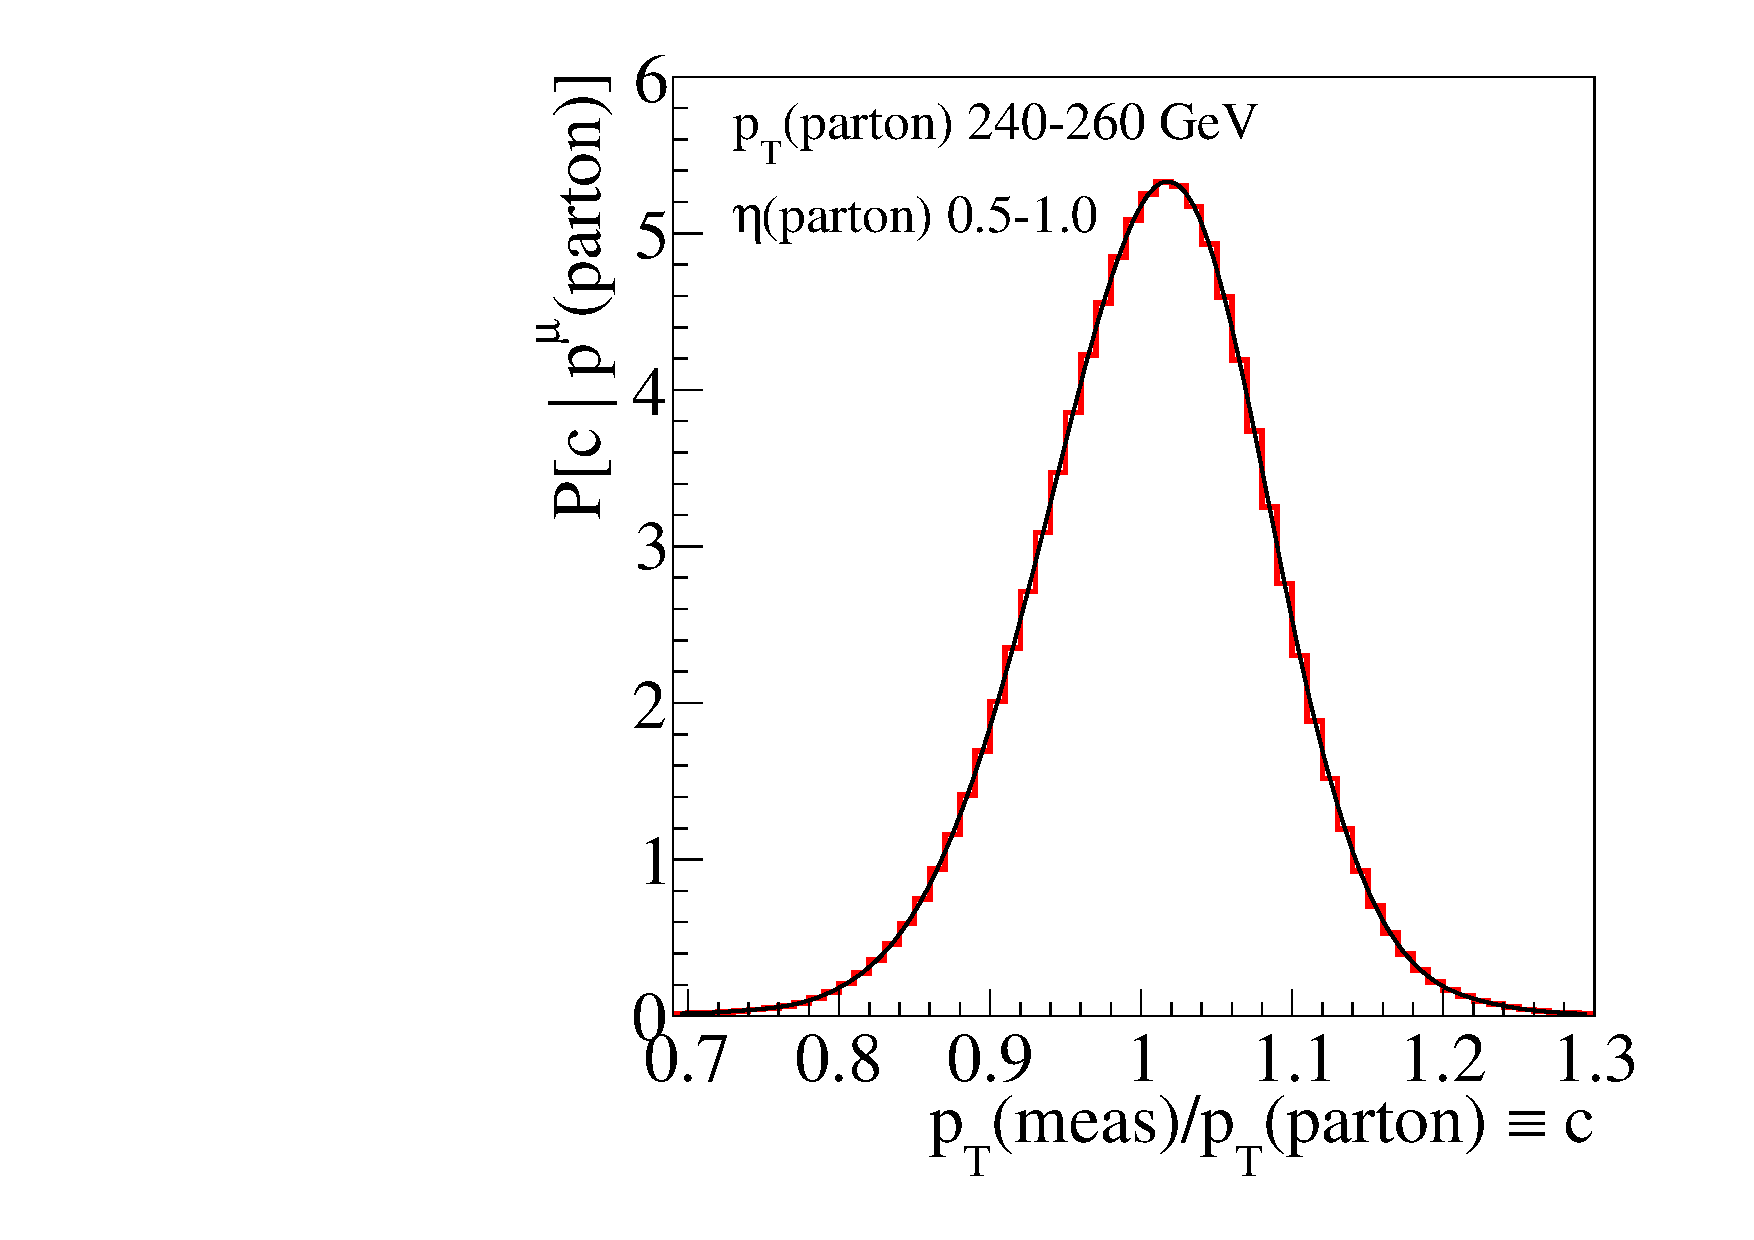
\includegraphics[width=0.5\linewidth]{figures/SusySearches/Ra2b2016/SmearEx2.pdf}
}
\caption{The likelihood function for the jet energy scale factor in two regions of the phase space of the parton-level jet four-vector. These distributions are equivalent to the smearing templates. The histograms (red) are smoothly interpolated using splines (black).}
\label{fig:SmearEx}
\end{figure}


\subsection{Rebalance and smear method}
The rebalance and smear method, originally developed by the authors of the Dissertations~\cite{Koay:2011qqa}\cite{Schroder:2012lqa}\cite{Goebel:2015kca} and the paper~\cite{Chatrchyan:2014lfa}, exploits the relationships given in Equations \ref{eq:metTrue}, along with the jet energy resolution, to form a transfer function between the measured and parton-level jets. The first step of the method is to identify the optimal matrix of scale factors $\hat{C}$ that transforms the collection of reconstruction-level jets into a set that resembles a parton-level jet collection, and (historically) yields an event with $\mht=0$; jets in the resulting collection are referred to as the rebalanced jets. In the second step, the four-vectors of the rebalanced jets are smeared according to the likelihood for the scale factor given in Equation \ref{eq:JetEnergyLikelihood}. This procedure, applied to all events in a QCD-enriched data control sample, yields event sample that is the basis of the QCD background prediction. Predictions for the QCD background in the signal regions are derived from cuts applied to this sample, which we may refer to as the prediction event sample. I have adapted key aspects of the methodology, which I will now describe step-by-step.

\subsubsection{Rebalance procedure: a Bayesian approach}
In the re-envisioned approach to the rebalancing procedure,  it is possible to systematically  incorporate prior knowledge about the true $\mht$ distribution and jet response functions to constrain the jets. The objective is to rebalance the collection of measured jets so that it resembles a parton-level collection. An inversion of the likelihood function for the jet energy scale factors is performed using Bayes' theorem (see the Chapter \ref{chap:run1pmssm} for a brief introduction). The probability density for the parton-level jet collection can be written as
\begin{equation}
{\rm P}(\vec{J}_{\rm part}|\vec{J}_{\rm meas}) \sim {\rm P}(\vec{J}_{\rm meas}|\vec{J}_{\rm part})\cdot \pi(\vec{J}_{\rm part}),
\label{eq:posterior1}
\end{equation}
where $\pi(\vec{J}_{\rm part})$ is the $n$-dimensional prior probability density for the parton-level jet collection.
Treating the jets as mutually independent allows the likelihood to be factorized as
\begin{align}
\begin{split}
{\rm P}(\vec{J}_{\rm meas}|\vec{J}_{\rm part}) = \prod_{i=1}^{\njets}L_{i} &= \prod_{i=1}^{\njets}{\rm P}(p^{\mu}_{i,\rm meas}\ |\ p^{\mu}_{i,\rm part})\\
&=\prod_{i=1}^{\njets}{\rm P}(c_i\ |\ p^{\mu}_{i,\rm part}).
\end{split}
\label{eq:likelihood1}
\end{align}
The prior allows our knowledge about the parton-level missing transverse energy outlined in Equation \ref{eq:metTrue} to constrain the rebalance of the jets. However, while equations \ref{eq:metTrue} are true for the $E_{T}^{\rm miss}$, the analysis at hand uses the missing transverse hadronic energy $\mht$, defined as
\begin{equation}
\vec{H}_{T}^{\rm miss} \equiv -\sum_{i=1}^{{\rm N}_{\rm jet}}(\vec{p}_{T})_{i}\cdot\Theta(30{\rm\ GeV}-(p_{T})_{i}).
\end{equation}
The threshold on the $p_{T}$ applied via the Heaviside function to remove jets originating from pileup interactions spoils the equality in Equation \ref{eq:metTrue}. Jets with $p_{T}$ less than 30 GeV can recoil off harder jets, and this produces non-zero true $\mht$. However, the parton-level $\mht$ is still small compared to the reconstruction-level $\mht$, as seen in the distribution of parton- and reconstruction-level $\mht$ in Figure \ref{fig:Mht}, implying that the underlying $\mht$ distribution may provide a meaningful constraint on our knowledge of the parton-level system. A difference is also seen in the angular distribution of the $\mht$, in the polar coordinate system with the z-axis defined along the direction of the leading jet, and this information can likewise be incorporated, as will now be demonstrated.
\begin{figure}[h]
\centering
\subfloat[]{
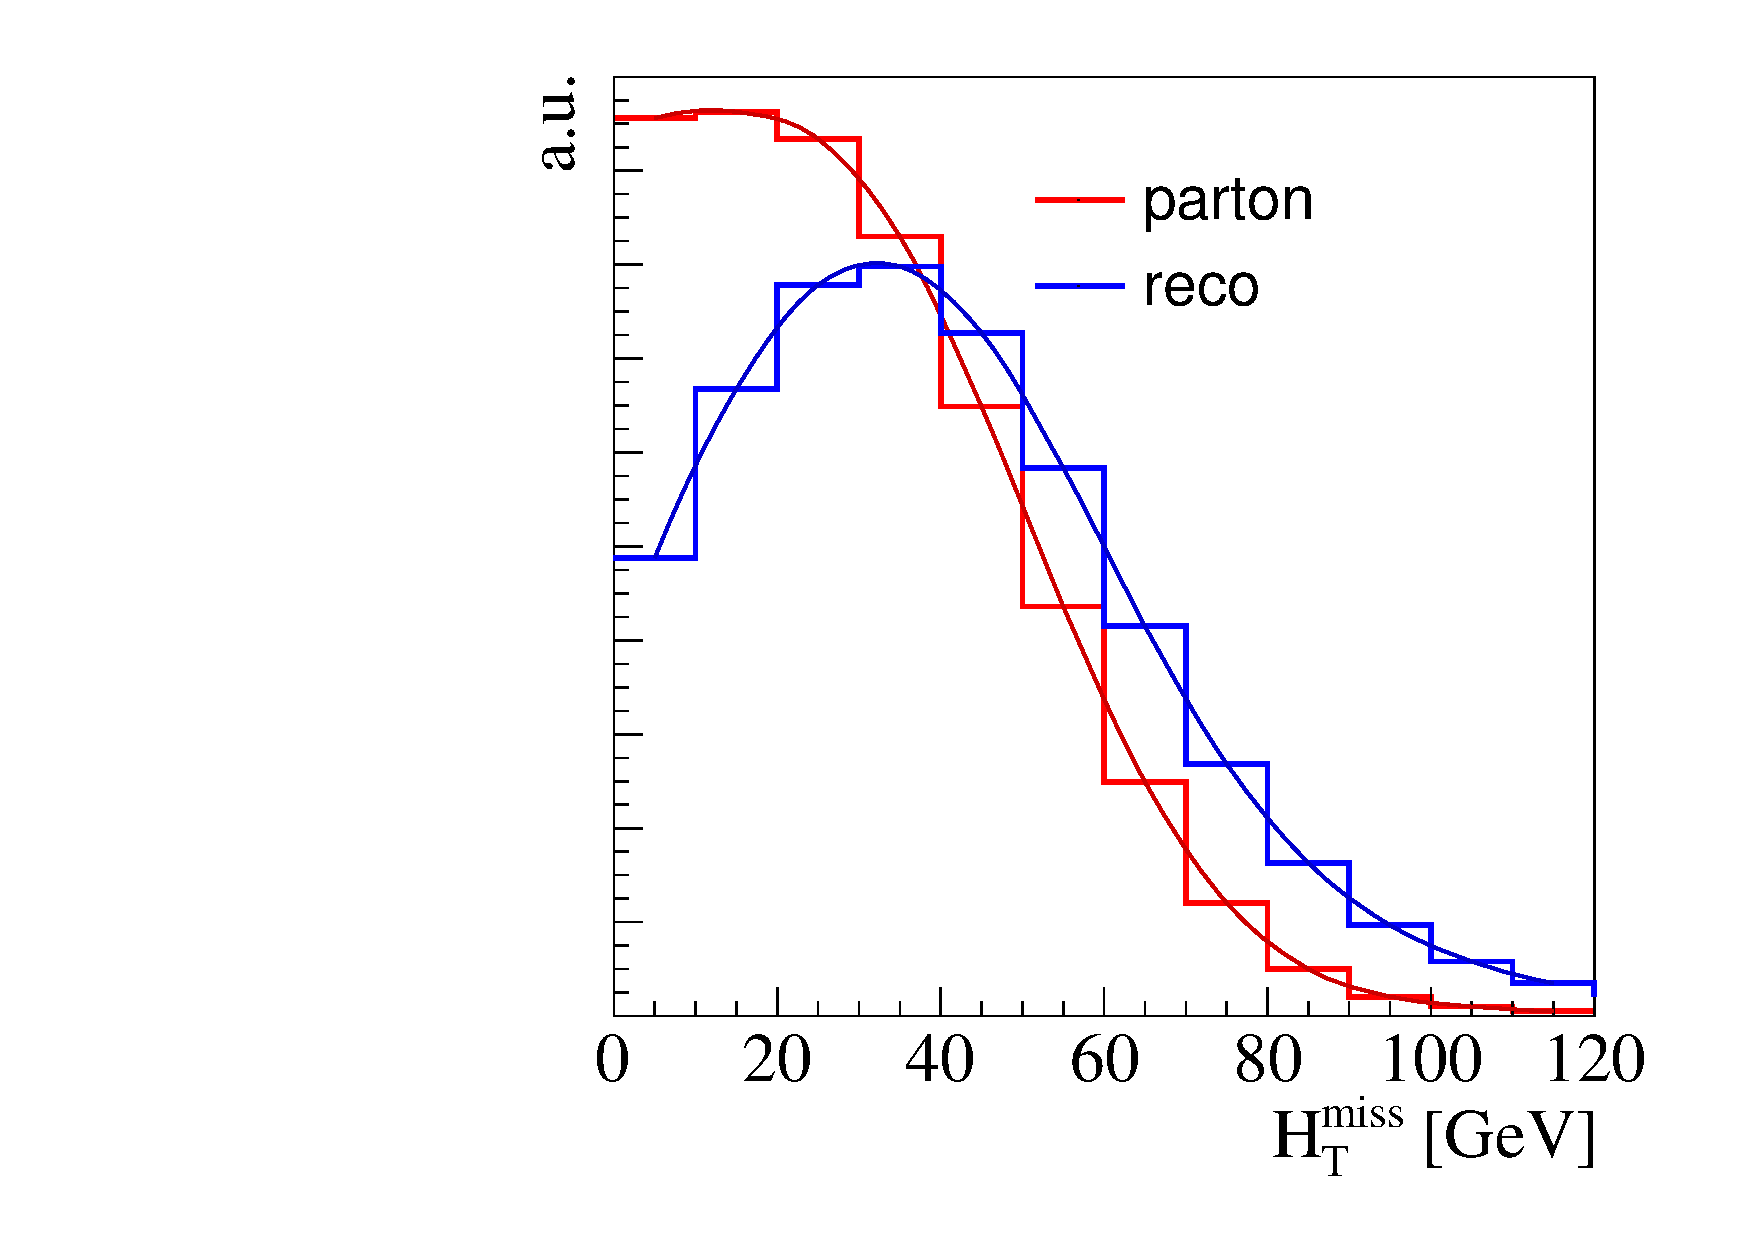
\includegraphics[width=0.5\linewidth]{figures/SusySearches/Ra2b2016/MhtGenAndTruth.pdf}
}
\subfloat[]{
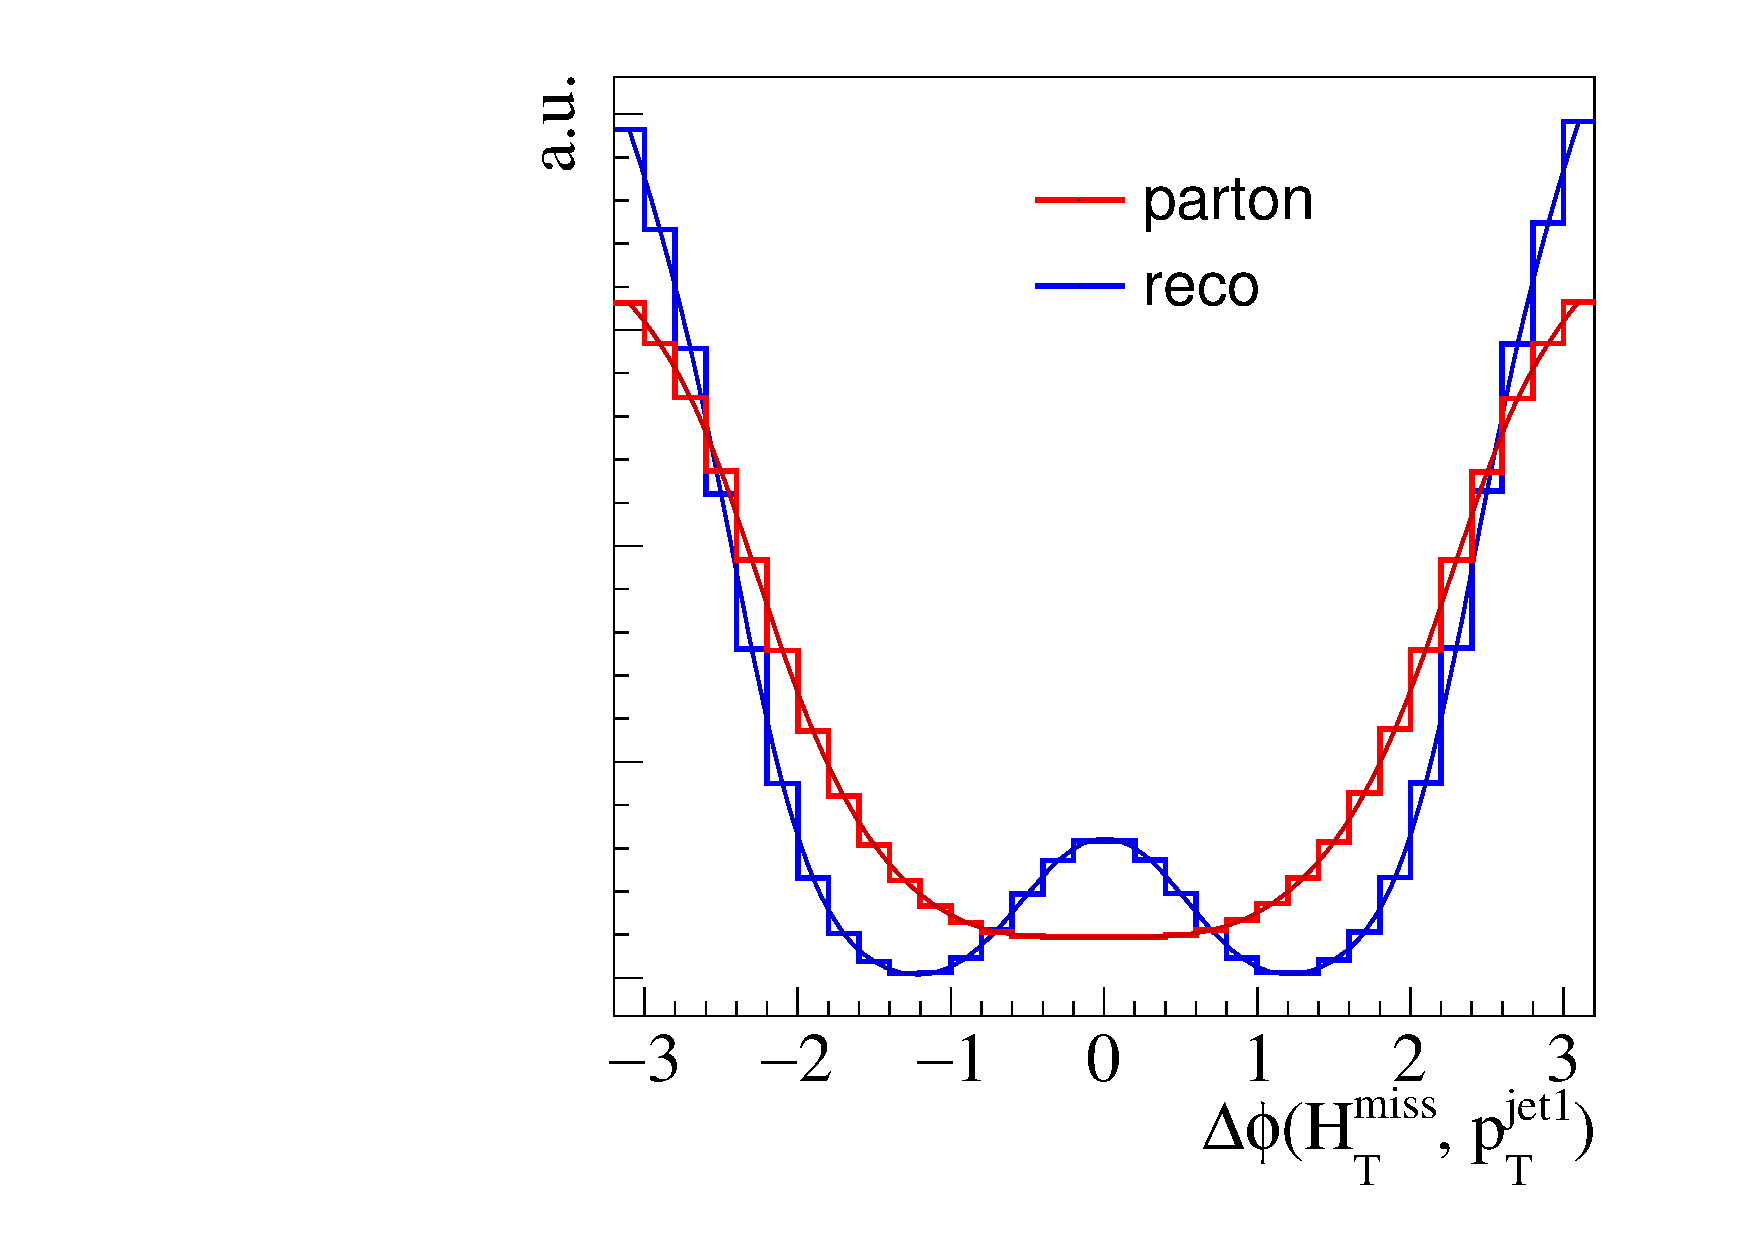
\includegraphics[width=0.5\linewidth]{figures/SusySearches/Ra2b2016/DPhiMhtJet1GenAndTruth.pdf}
}
\caption{The parton-level and reconstruction-level $\mht$ and azimuthal separation between the $\mht$ and leading jet in QCD simulation. The red functions are taken as probability distributions making up the prior, $\text{P}[\mht(\vec{J}_{\rm part})]$ and $\text{P}[\Delta\phi_{\mht,p_{T}^1}(\vec{J}_{\rm part})]$}
\label{fig:Mht}
\end{figure}

The parton-level information contained in the red distributions can be incorporated into the posterior density via an expression relating the $\mht$ to the jet energy scale factors, and taking the red distributions to be factors in the prior. The templates for the $\Delta\phi$ between the $\mht$ and the leading jet are derived separately in bins of the b-jet multiplicity, for the bins of 0, 1, and $\geq$ 2 b-jets.  This choice and its implications are discussed later. For the case where there are one or more b-jets, the $\Delta\phi$ between the $\mht$ and the leading b-jet is used. Combining Eqs. \ref{eq:posterior1}, \ref{eq:likelihood1} gives
\begin{equation}
{\rm P}(\vec{J}_{\rm part}|\vec{J}_{\rm meas}) \sim
\prod_{i=1}^{\njets}{\rm P}(p^{\mu}_{i,\rm meas}|p^{\mu}_{i,\rm part})\cdot \text{P}[\mht(\vec{J}_{\rm part})]\cdot \text{P}[\Delta\phi_{\mht,p_{T}^1}(\vec{J}_{\rm part})]\cdot \pi_0(\vec{J}_{\rm part}),
\end{equation}
where $\pi_0(\vec{J}_{\rm part})$ is the initial prior on the parton jet four-vectors, taken to be uniform. Having constructed a posterior density, the parton-level jets can be inferred by integrating with respect to the reconstruction-level jet four-vectors, or alternatively, by performing a likelihood maximization. The second approach is taken.


\subsubsection{Posterior density of jet momenta}
Bayes' theorem suggests that incorporating new relevant information will lead to improved knowledge about a system. In the case of the rebalance and smear method, we might expect a rebalanced event to more closely resemble the parton-level event than does the reconstruction-level event. Figure \ref{fig:rebareso} shows that the resolution of rebalanced jets is better than that of reconstructed jets by approximately 10\%.
\begin{figure}[h]
\centering
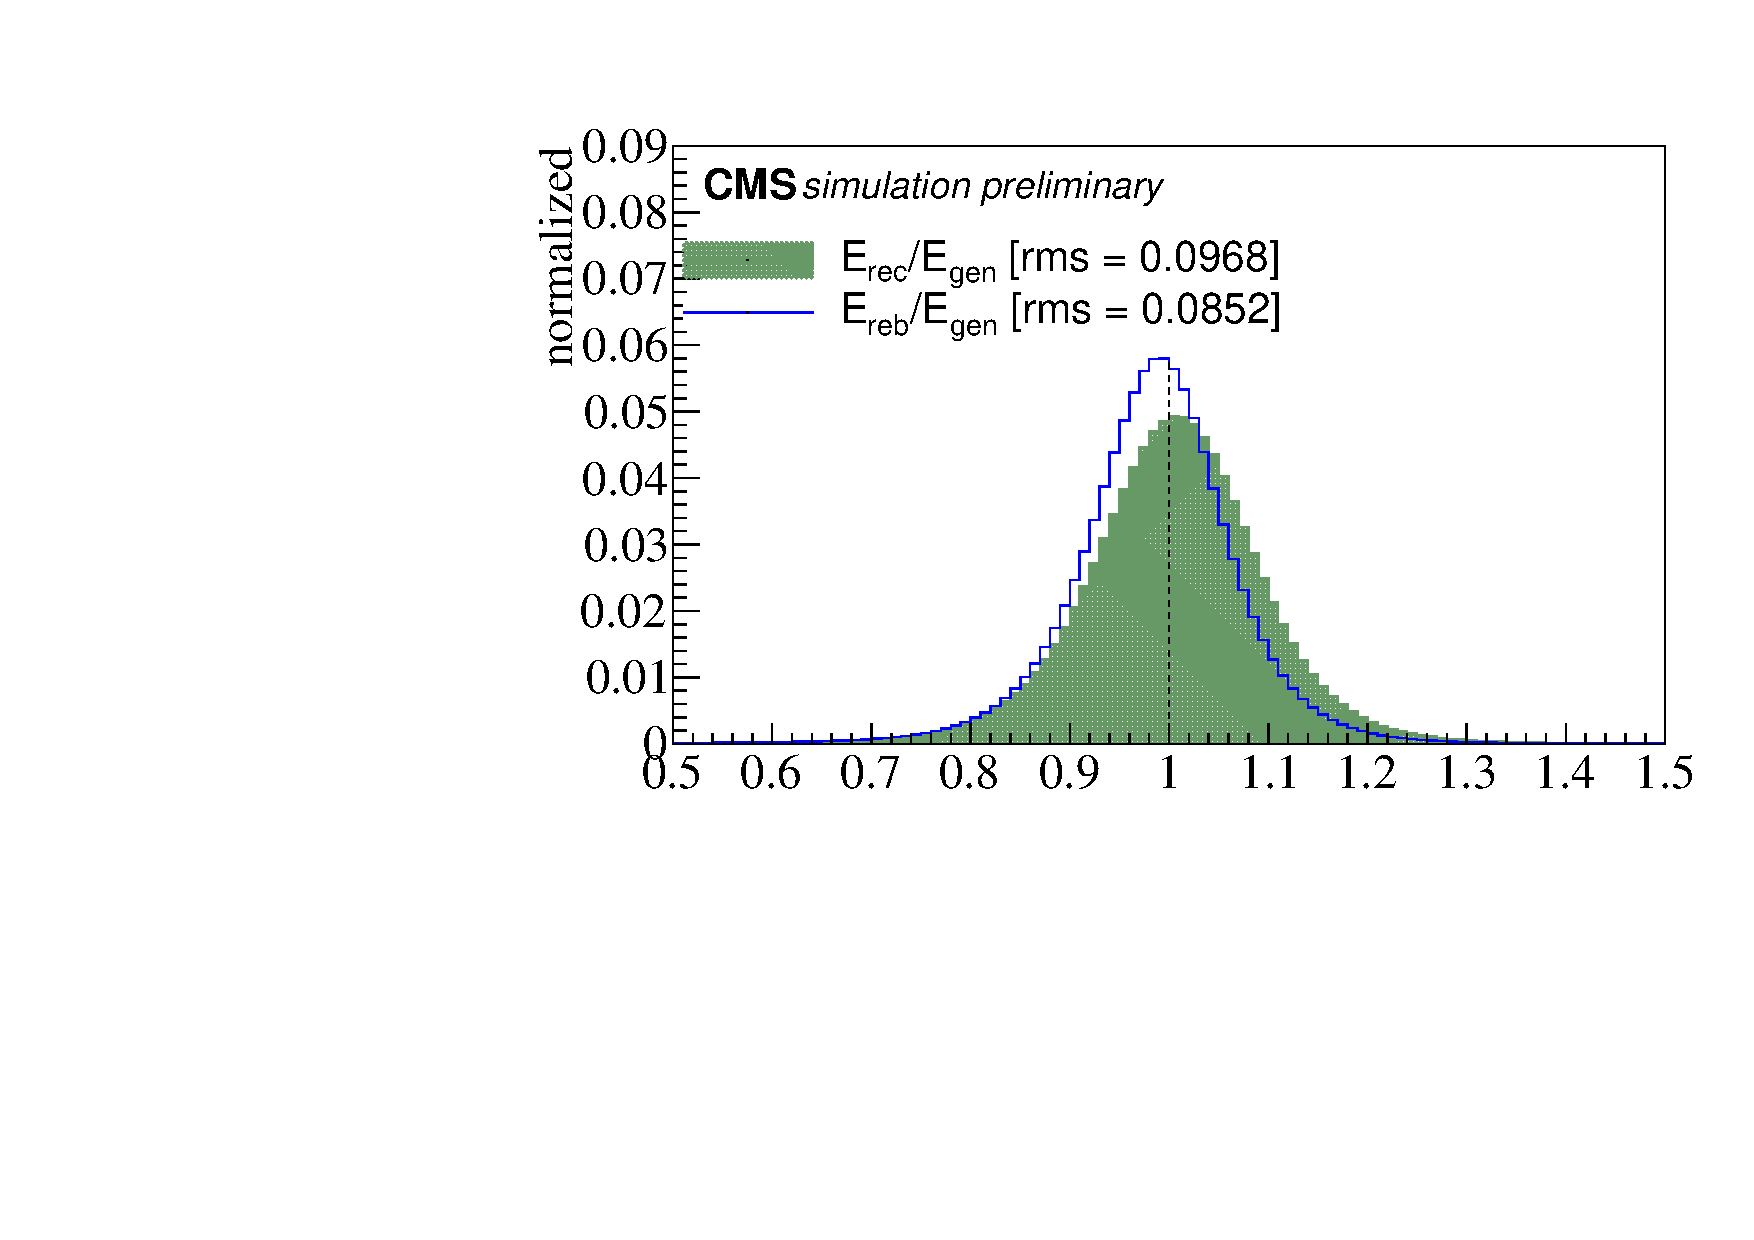
\includegraphics[width=0.49\linewidth]{figures/SusySearches/Ra2b2016/Jet1Resolution.pdf}
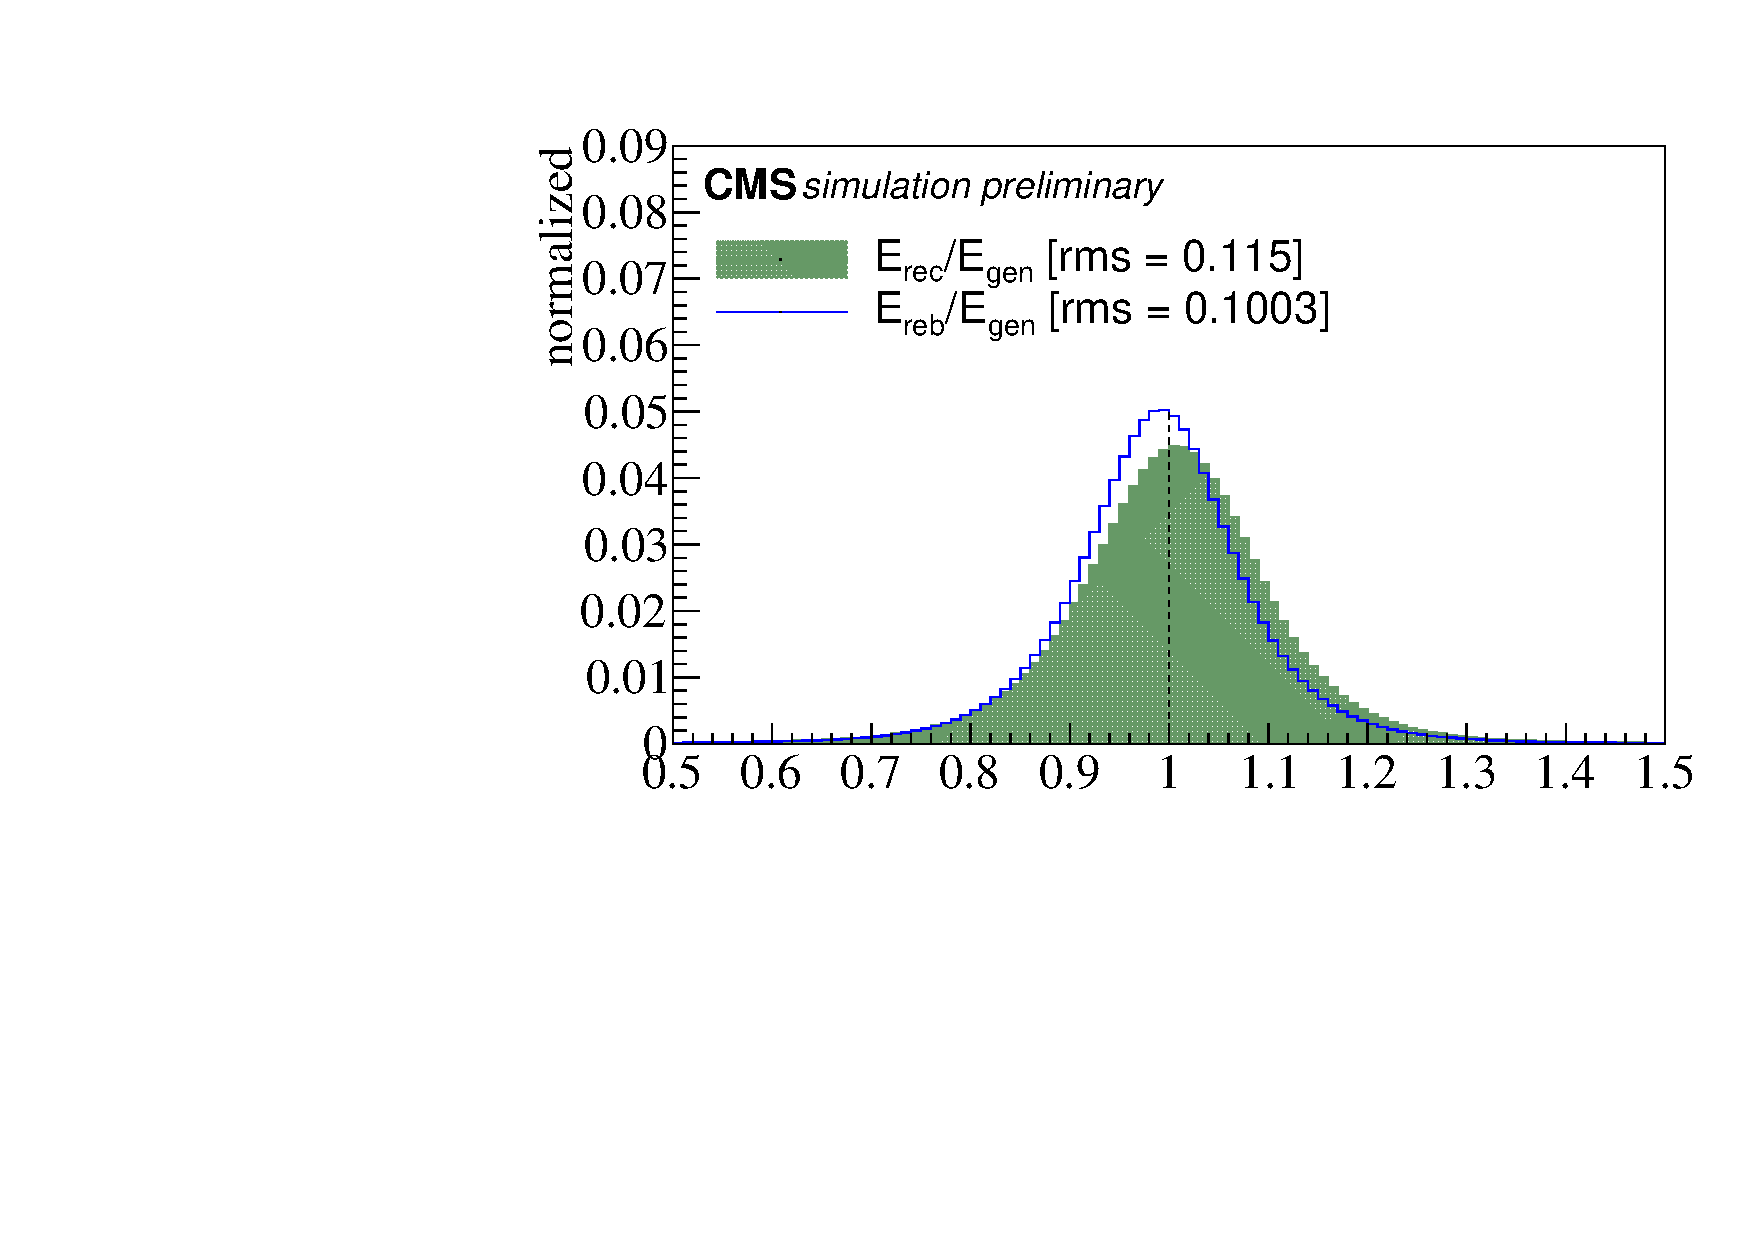
\includegraphics[width=0.49\linewidth]{figures/SusySearches/Ra2b2016/Jet2Resolution.pdf}
\caption{The jet energy response for the leading jet (left) and sub-leading jet (right) for reconstructed jets (green) and rebalanced jets (blue). Parton-level jets are required to have $\pt>30$ GeV and $|\eta|<2.4$. The resolution of rebalanced jets is better (smaller) than that of reconstruction-level jets by bout 10\%.}
\label{fig:rebareso}
\end{figure}
We also observe the peak of the response to be lower for rebalanced jets than for reconstructed jets. This is consistent with the peak of the jet $\pt$ likelihood functions being centered at values slightly higher than 1, as seen in Fig. \ref{fig:SmearEx}. 
\FloatBarrier

\subsubsection{Closure}
The rebalance and smear prediction is applied to simulated events and compared with the the result obtained directly from the simulation. Figures \ref{fig:BaselineRplusS} through \ref{fig:BaselineRplusS2} show this comparison for a number of observables after the baseline selection of the CMS multi-jet SUSY search, which is described in Section \ref{sec:2015results}. Then, Figs. \ref{fig:LowDeltaPhiRplusS} through \ref{fig:LowDeltaPhiRplusS2} show the comparison in the so-called inverted $\Delta \phi$ region, which has a selection equivalent to the baseline, but with the inverse of the selection on the $\Delta \phi$ between the $\mht$ and the jets. Figure \ref{fig:RplusSCorrelation} shows the comparison in two dimensions for selected pairs of observables. 

\begin{figure}[h]
\centering
\subfloat[]{
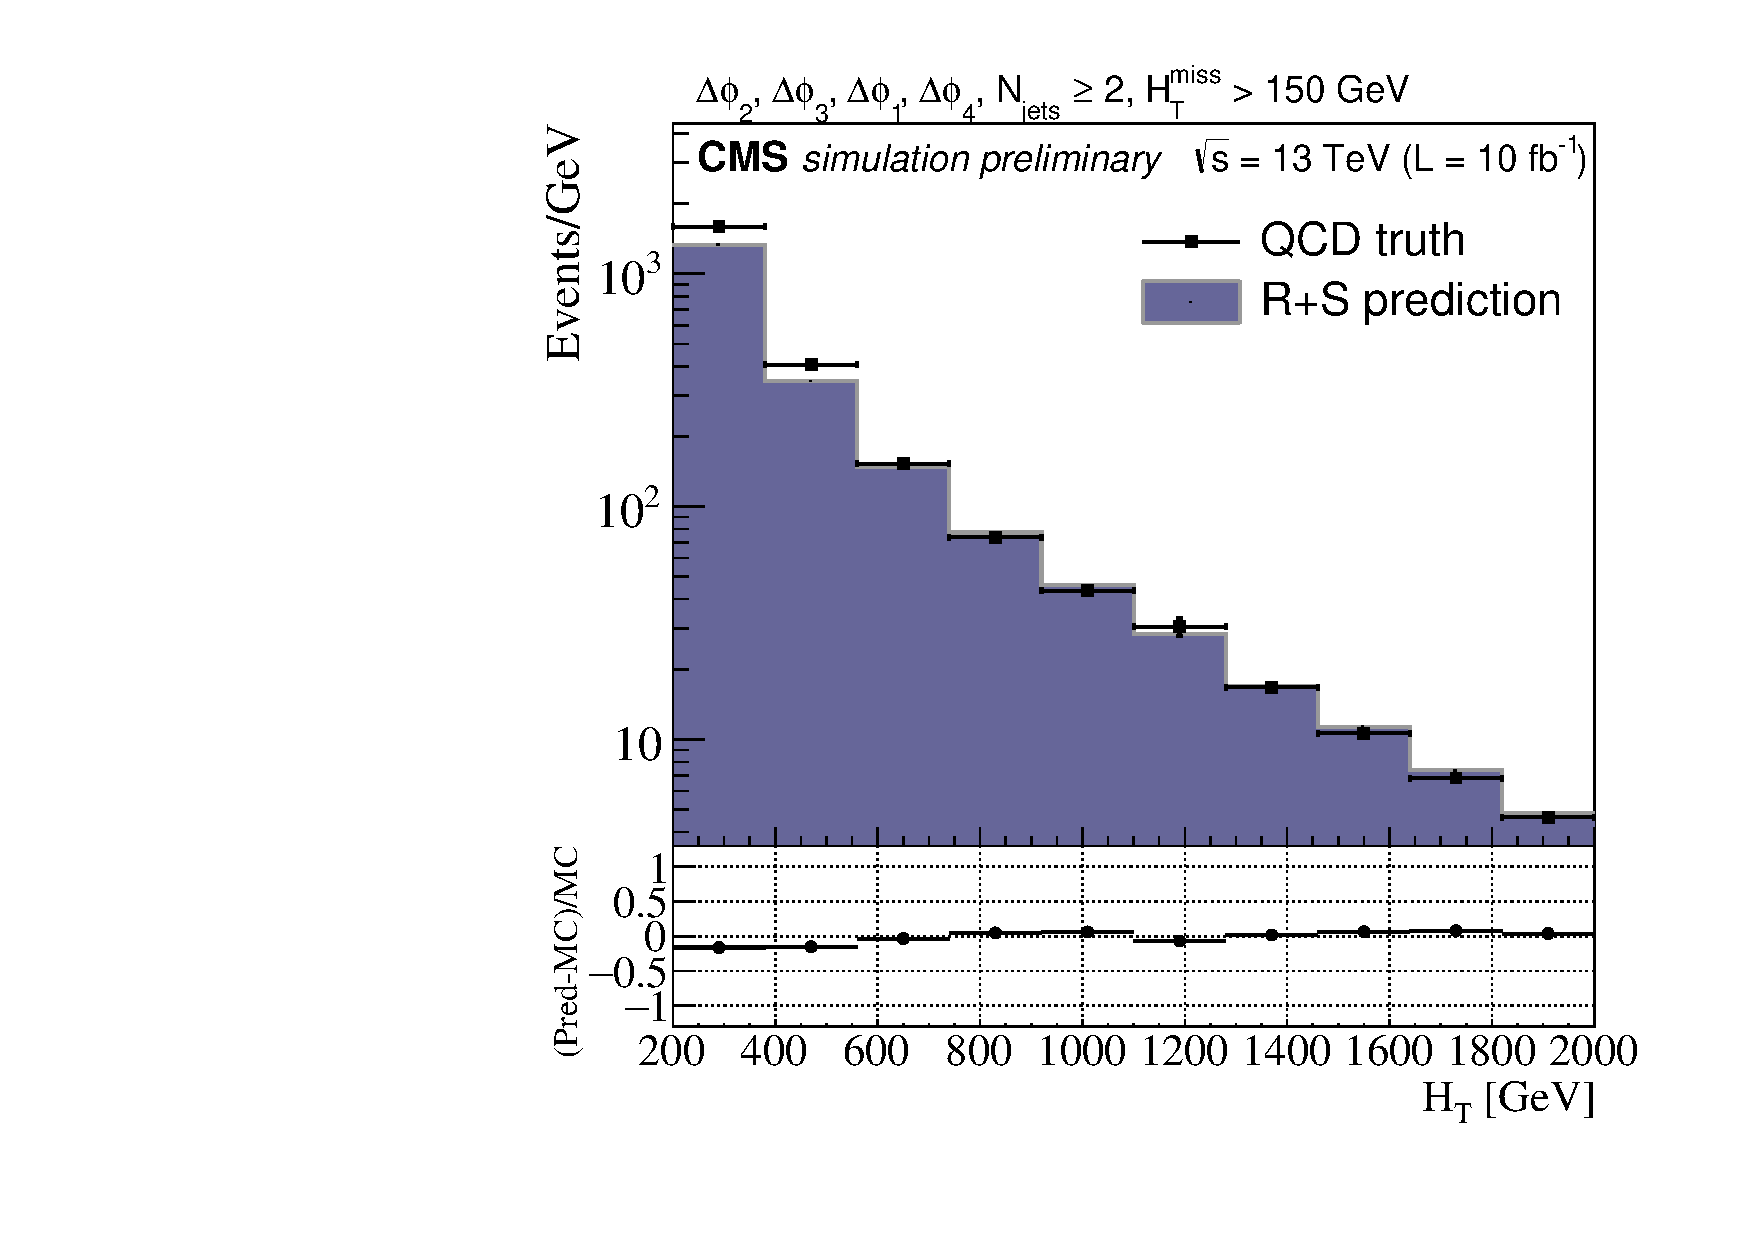
\includegraphics[width=0.5\linewidth]{figures/SusySearches/Ra2b2016/Baseline_Ht.pdf}
}
\subfloat[]{
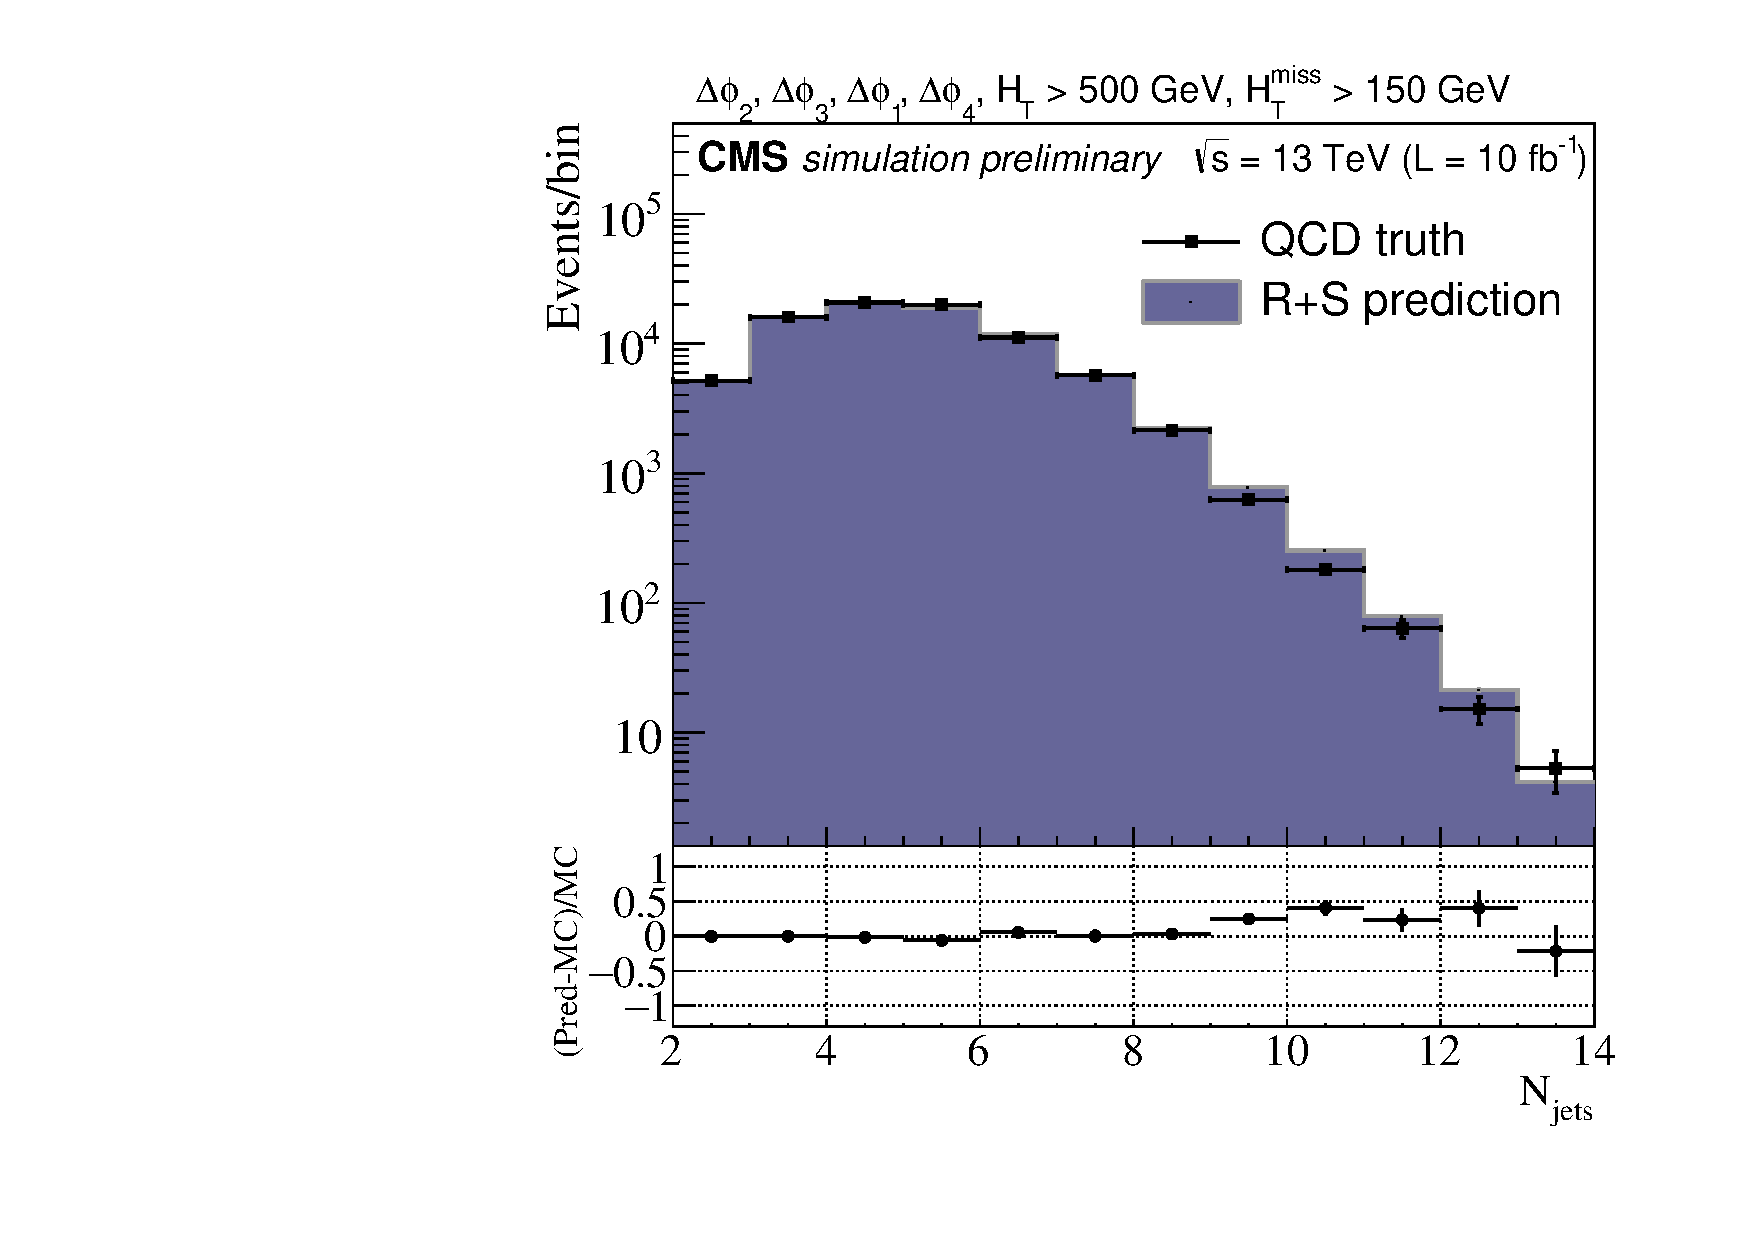
\includegraphics[width=0.5\linewidth]{figures/SusySearches/Ra2b2016/Baseline_NJets.pdf}
}\\
\subfloat[]{
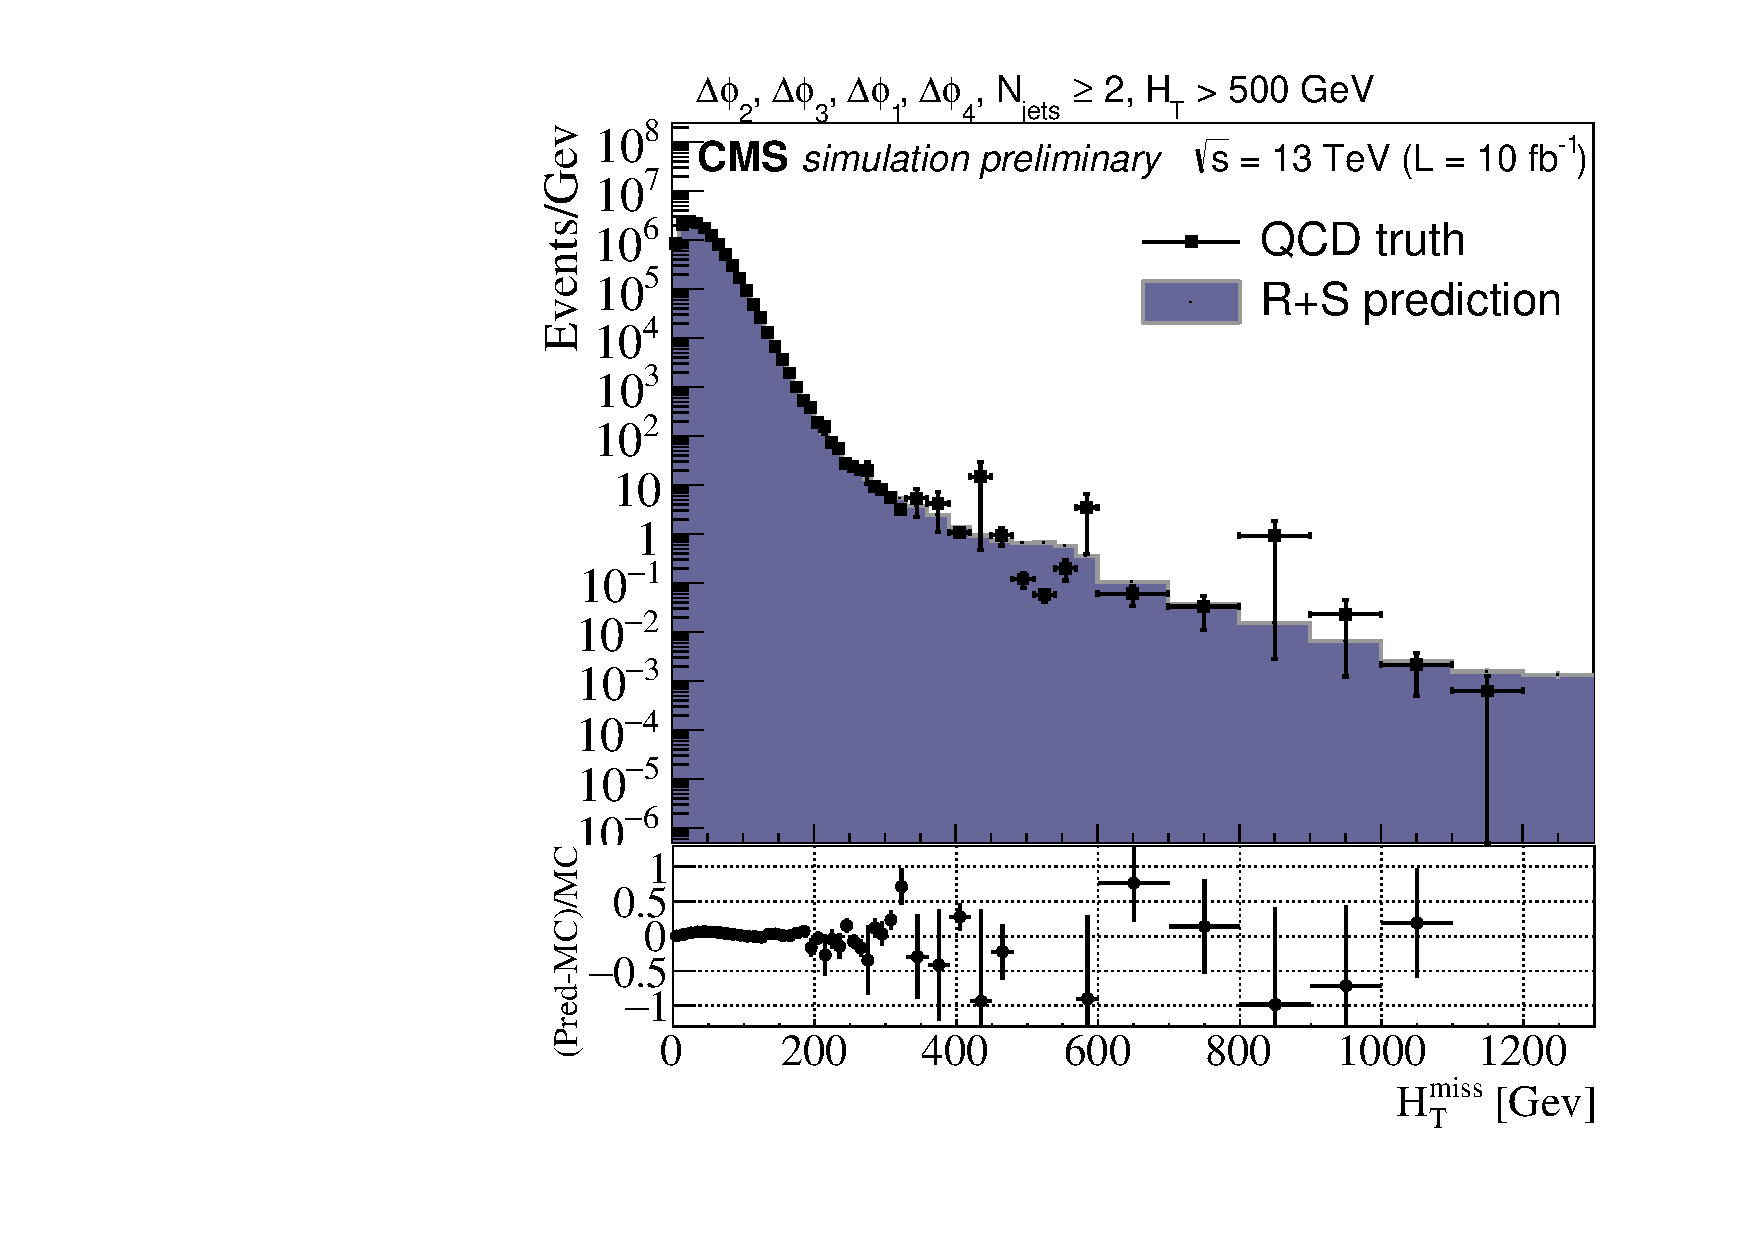
\includegraphics[width=0.5\linewidth]{figures/SusySearches/Ra2b2016/Baseline_Mht.pdf}
}
\subfloat[]{
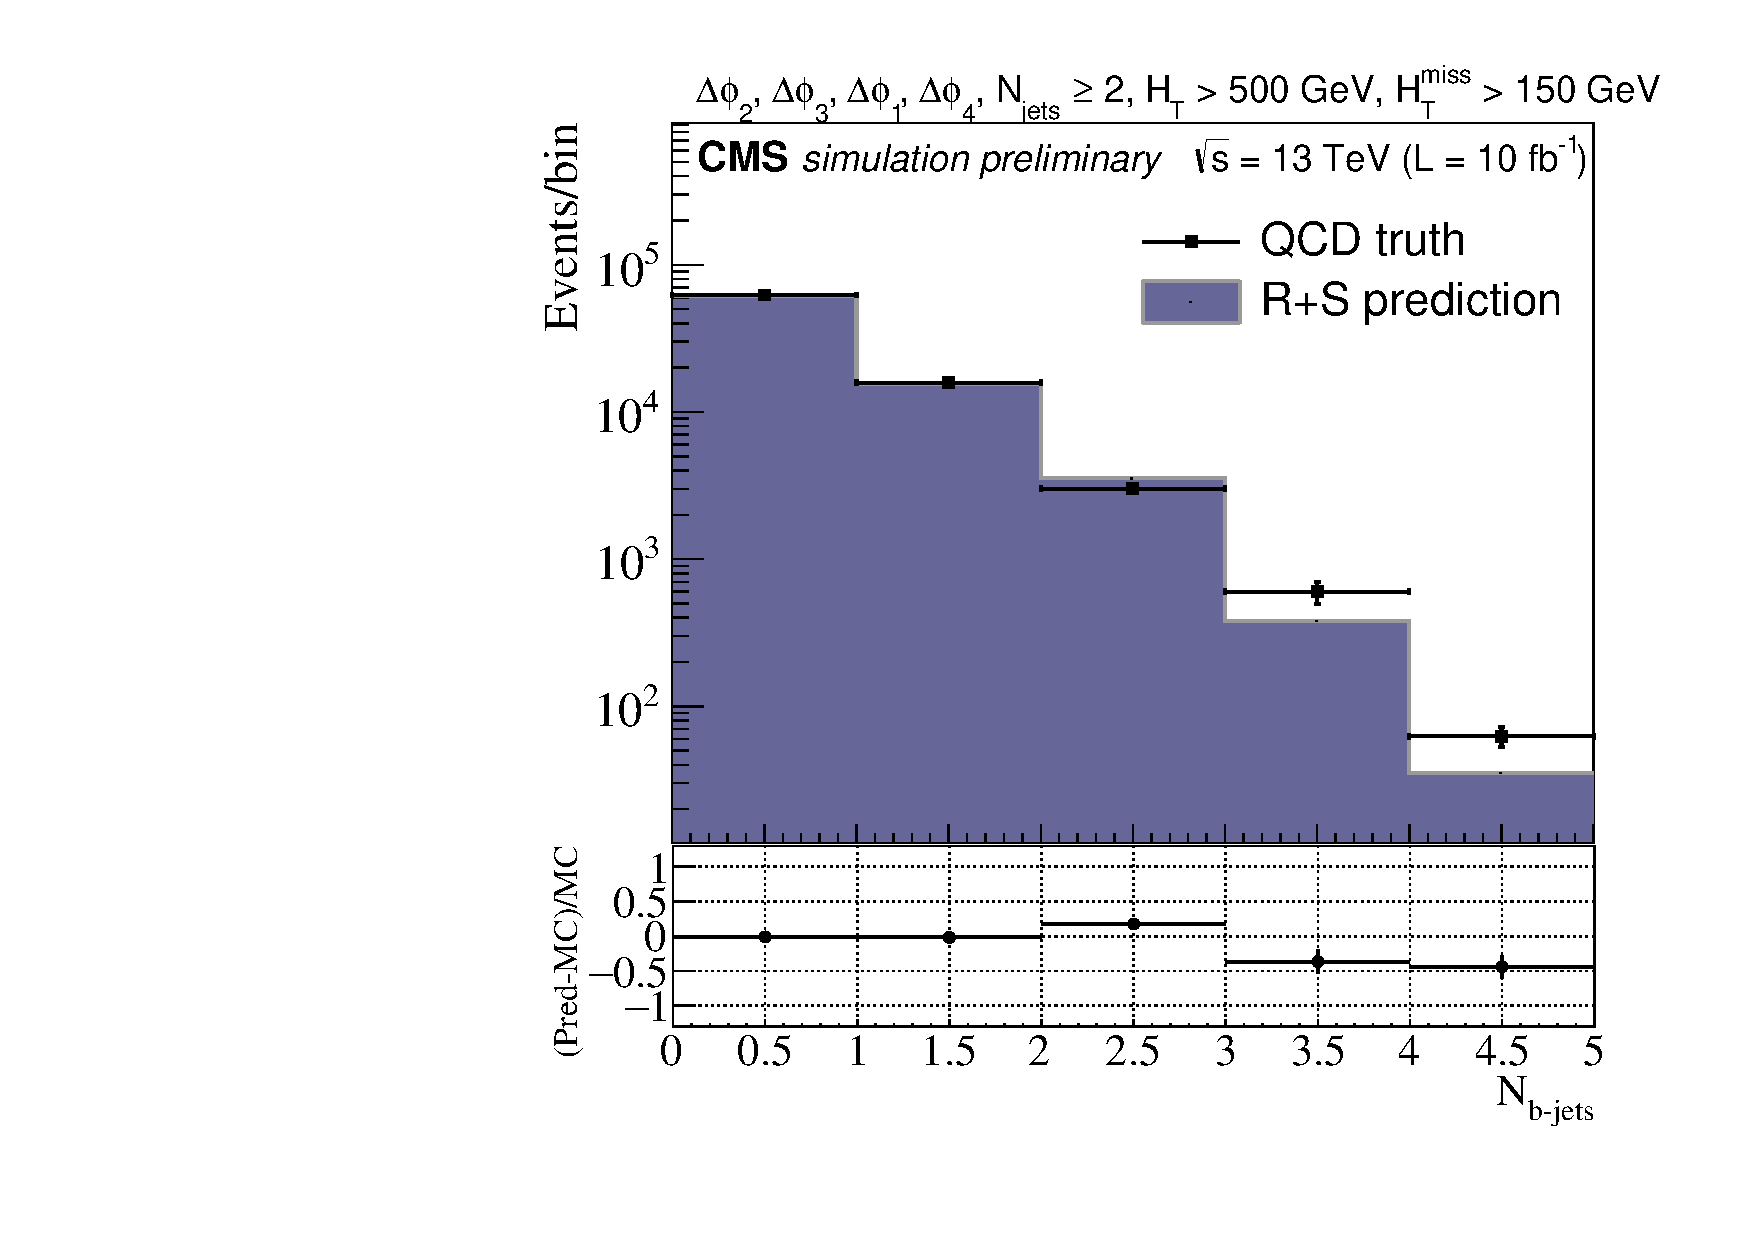
\includegraphics[width=0.5\linewidth]{figures/SusySearches/Ra2b2016/Baseline_BTags.pdf}
}
\caption{Comparisons of kinematic distributions between the direct simulation and the rebalance and smear method applied to simulation, after the baseline selection of the multi-jet SUSY search.}
\label{fig:BaselineRplusS}
\end{figure}

\begin{figure}[h]
\centering
\subfloat[]{
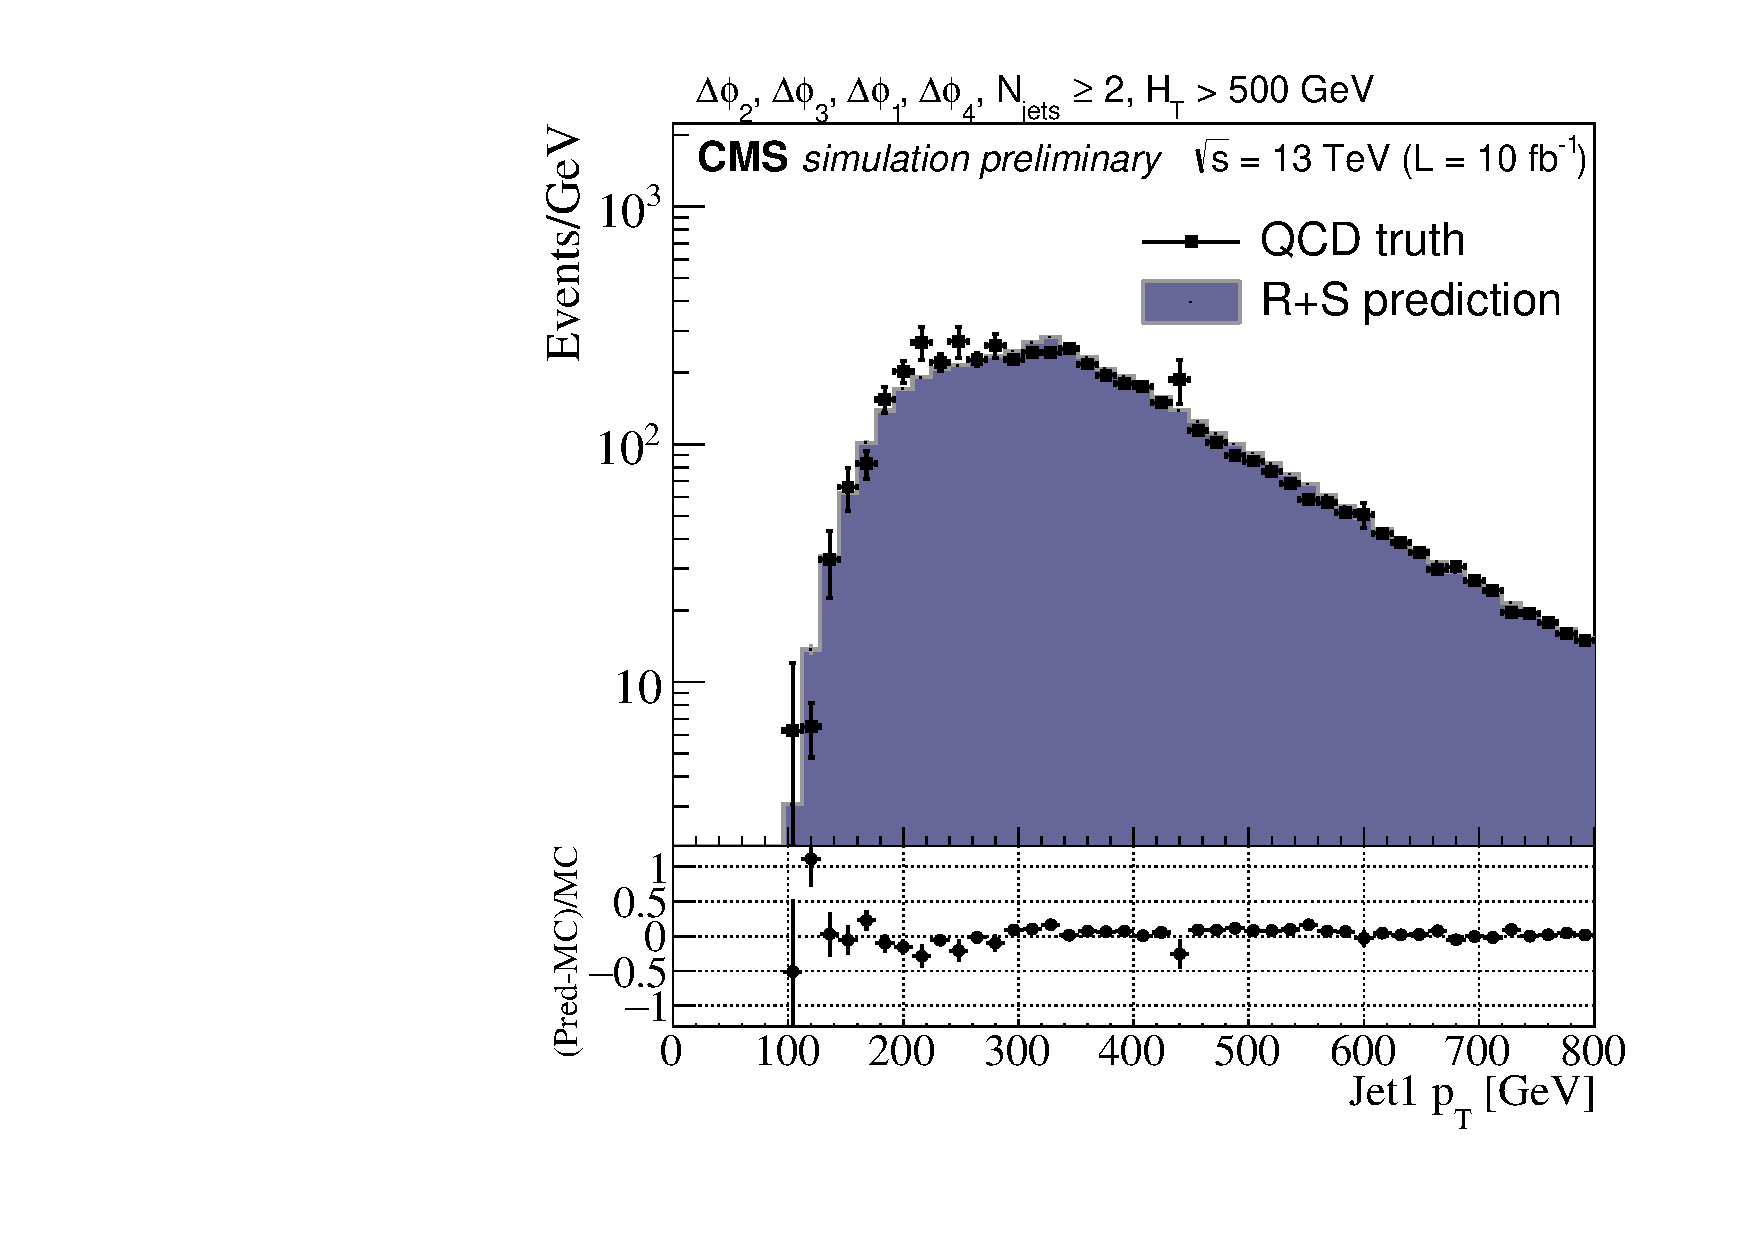
\includegraphics[width=0.5\linewidth]{figures/SusySearches/Ra2b2016/Baseline_Jet1Pt.pdf}
}
\subfloat[]{
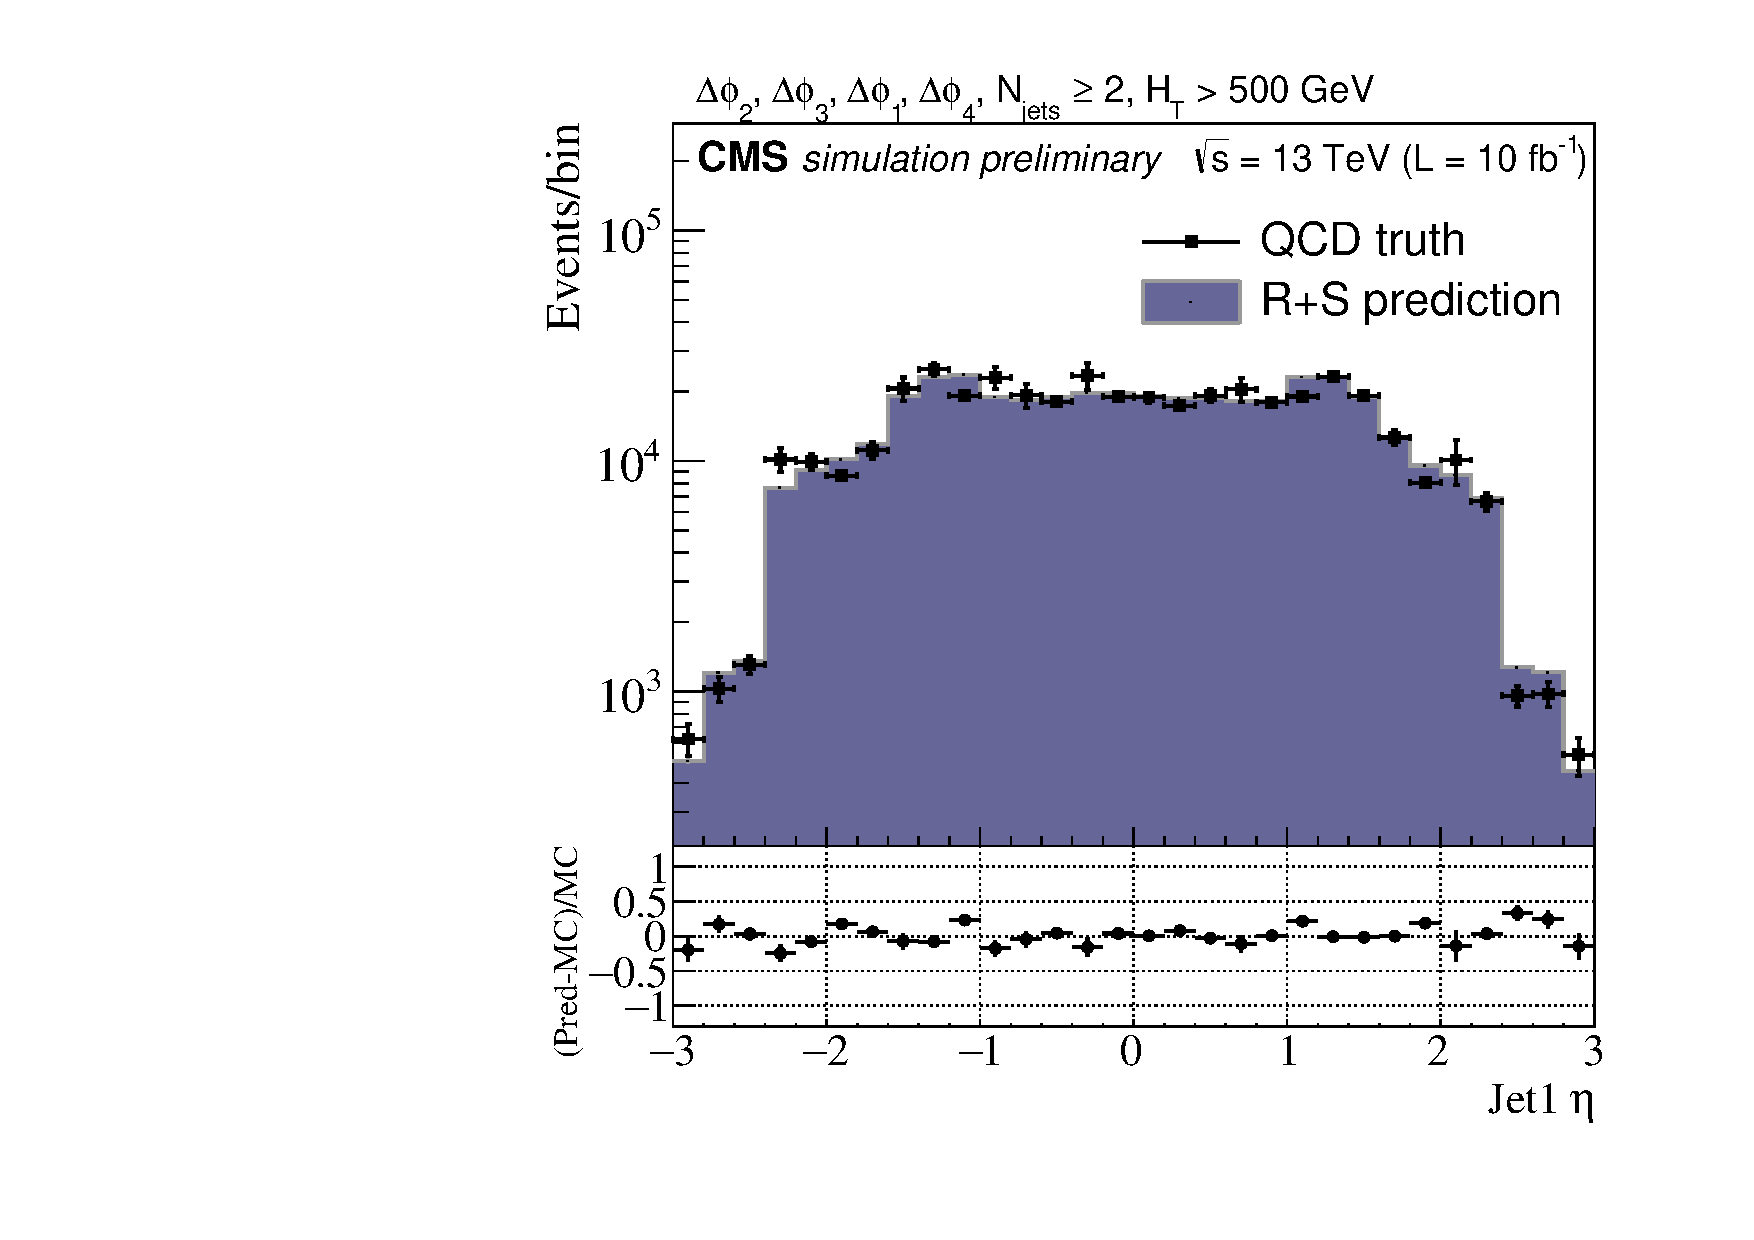
\includegraphics[width=0.5\linewidth]{figures/SusySearches/Ra2b2016/Baseline_Jet1Eta.pdf}
}\\
\subfloat[]{
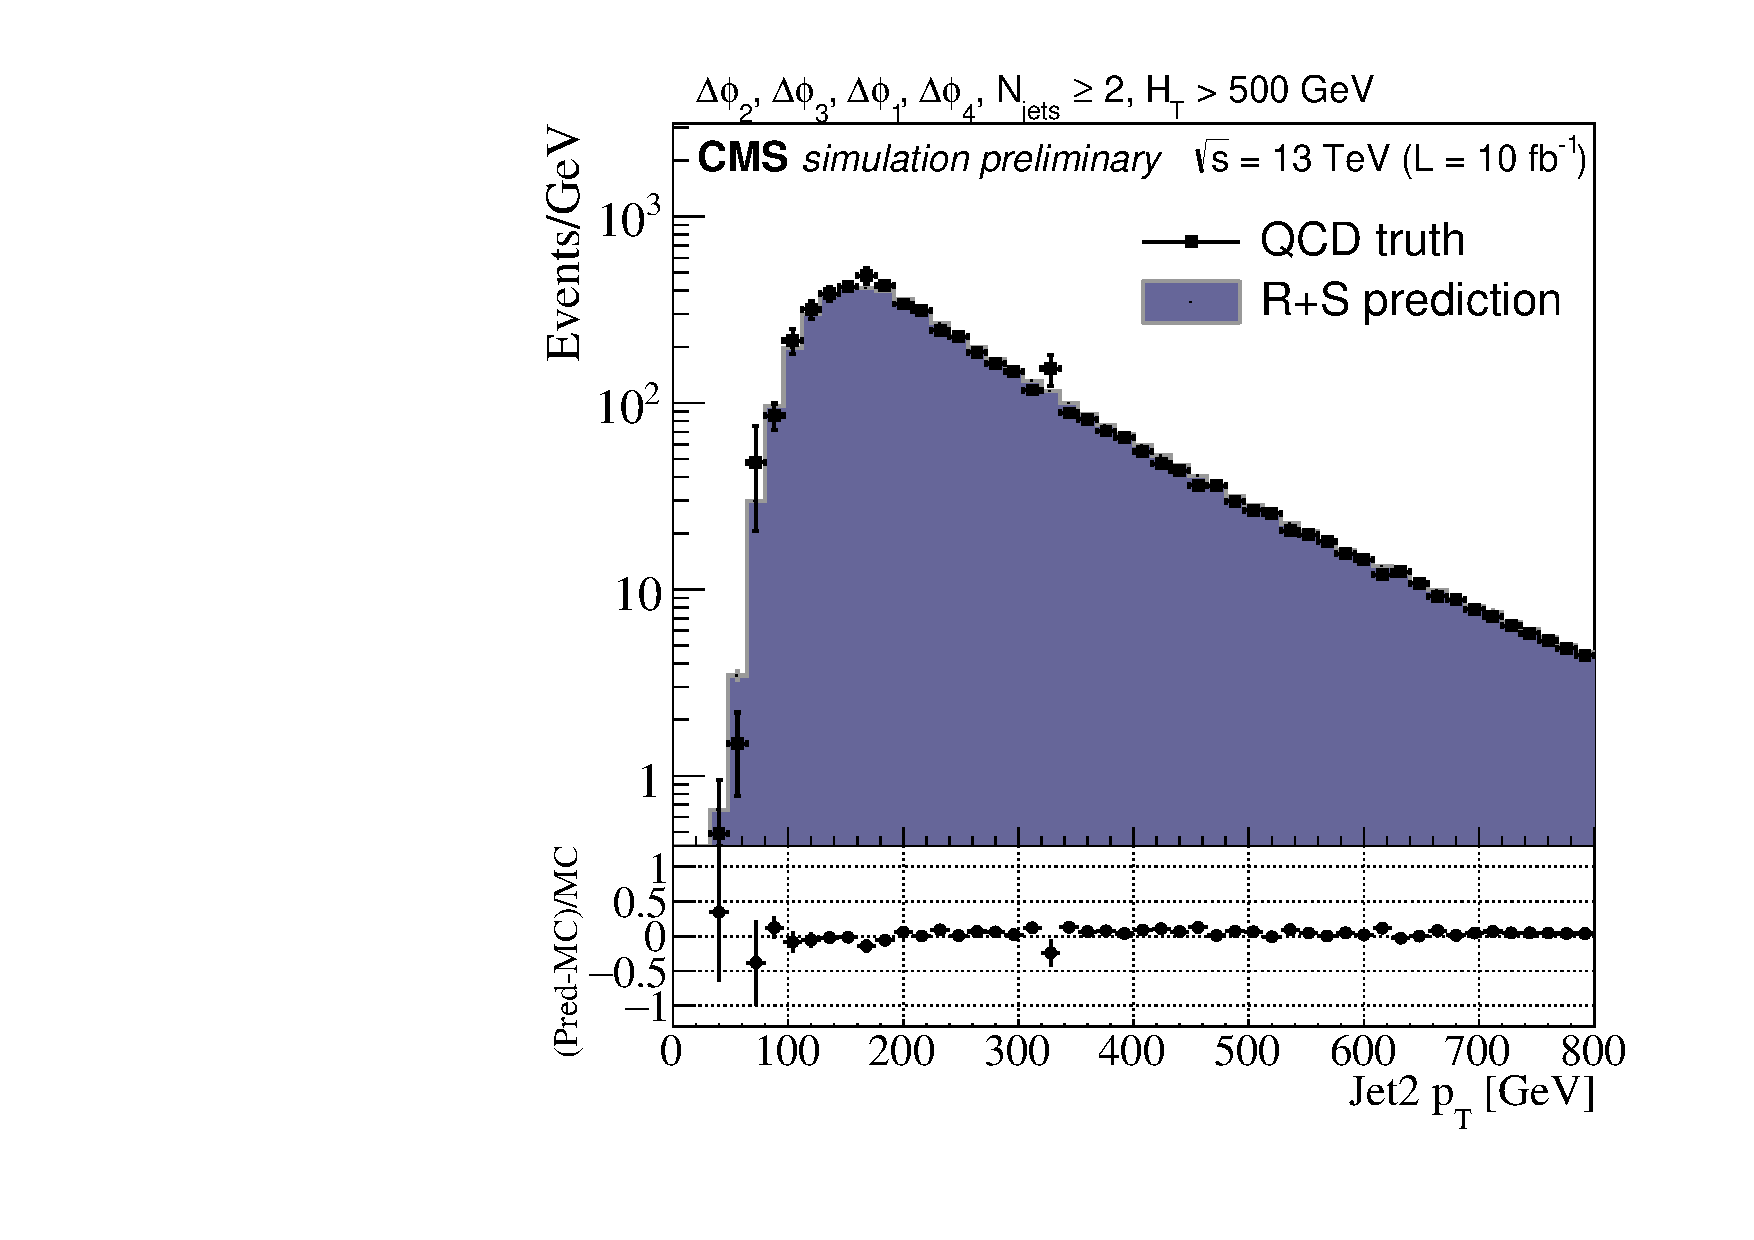
\includegraphics[width=0.5\linewidth]{figures/SusySearches/Ra2b2016/Baseline_Jet2Pt.pdf}
}
\subfloat[]{
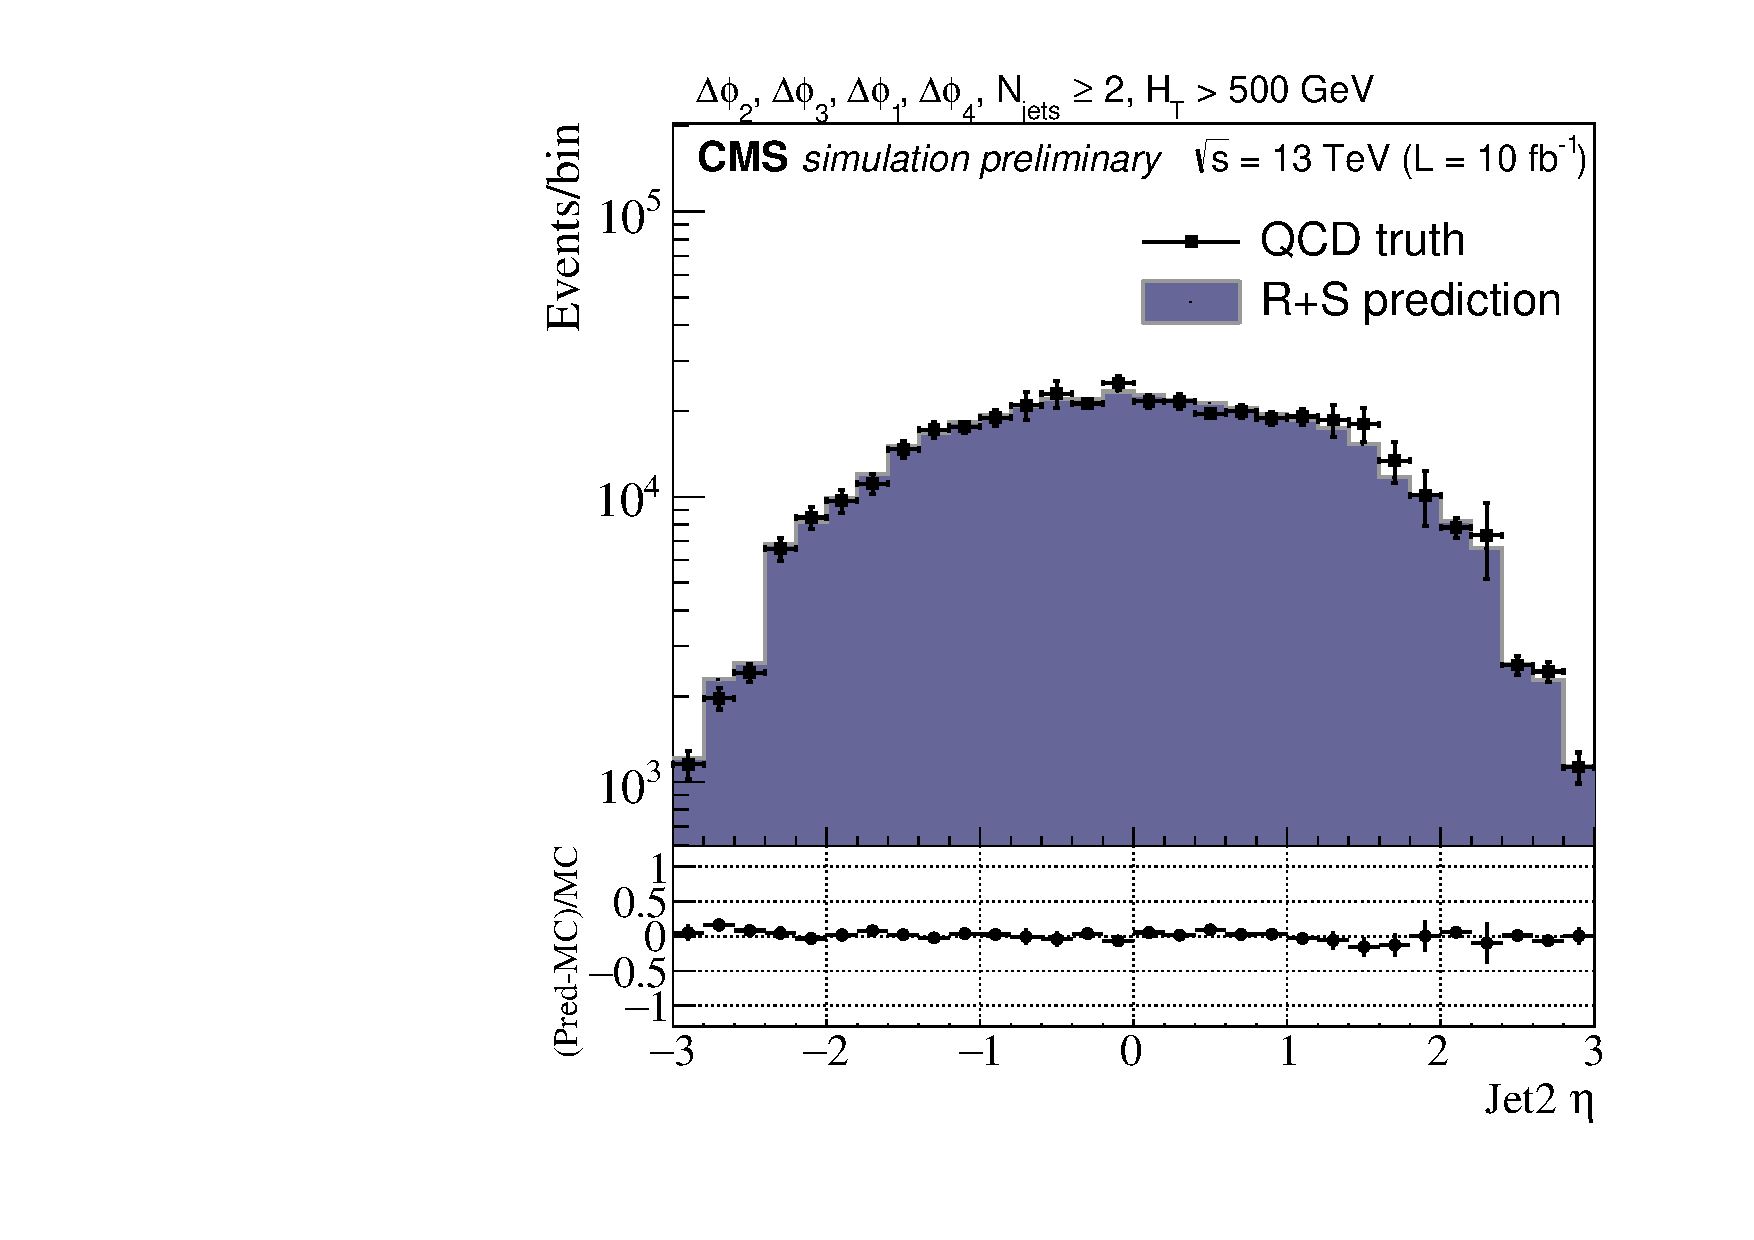
\includegraphics[width=0.5\linewidth]{figures/SusySearches/Ra2b2016/Baseline_Jet2Eta.pdf}
}
\caption{Comparisons of kinematic distributions between the direct simulation and the rebalance and smear method applied to the after the baseline selection of the multi-jet SUSY search.}
\label{fig:BaselineRplusSb}
\end{figure}


\begin{figure}[h]
\centering
\subfloat[]{
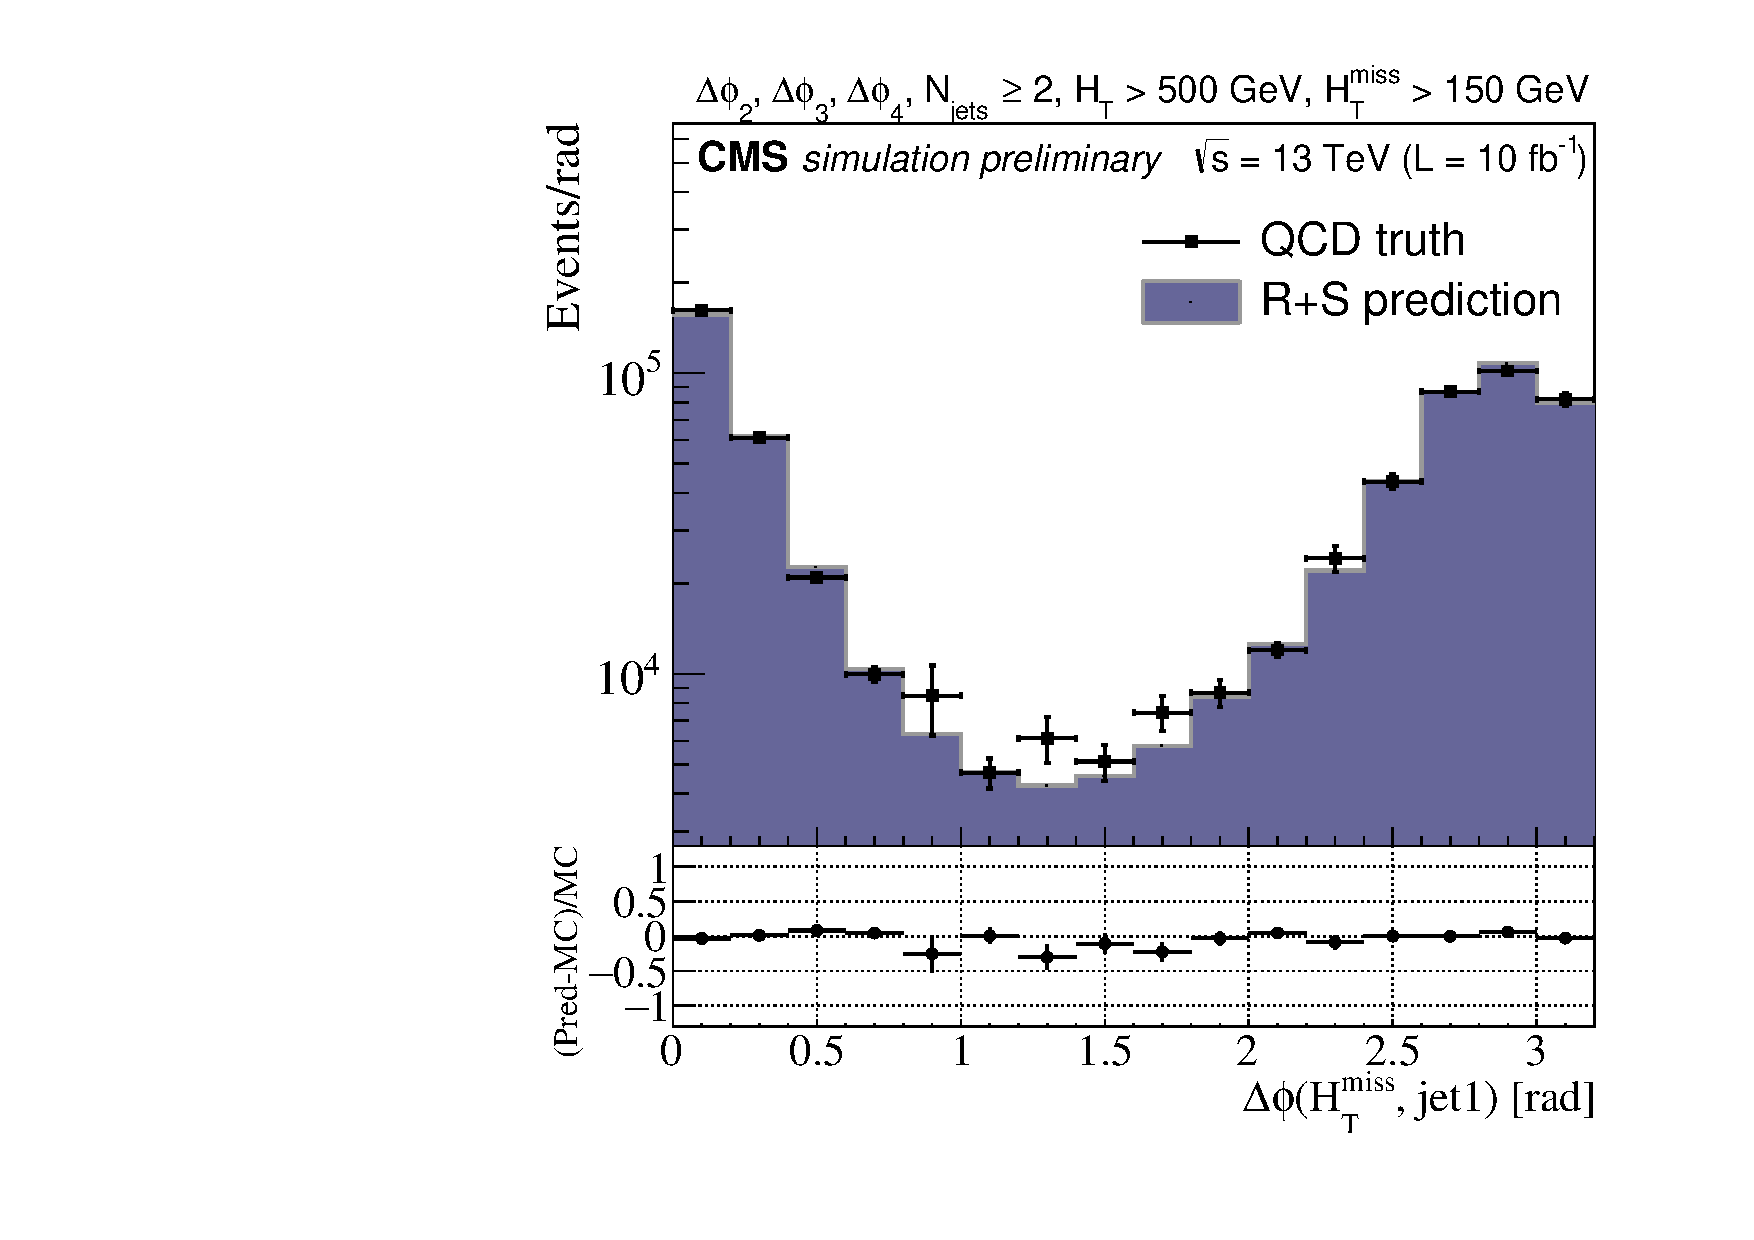
\includegraphics[width=0.5\linewidth]{figures/SusySearches/Ra2b2016/Baseline_DPhi1.pdf}
}
\subfloat[]{
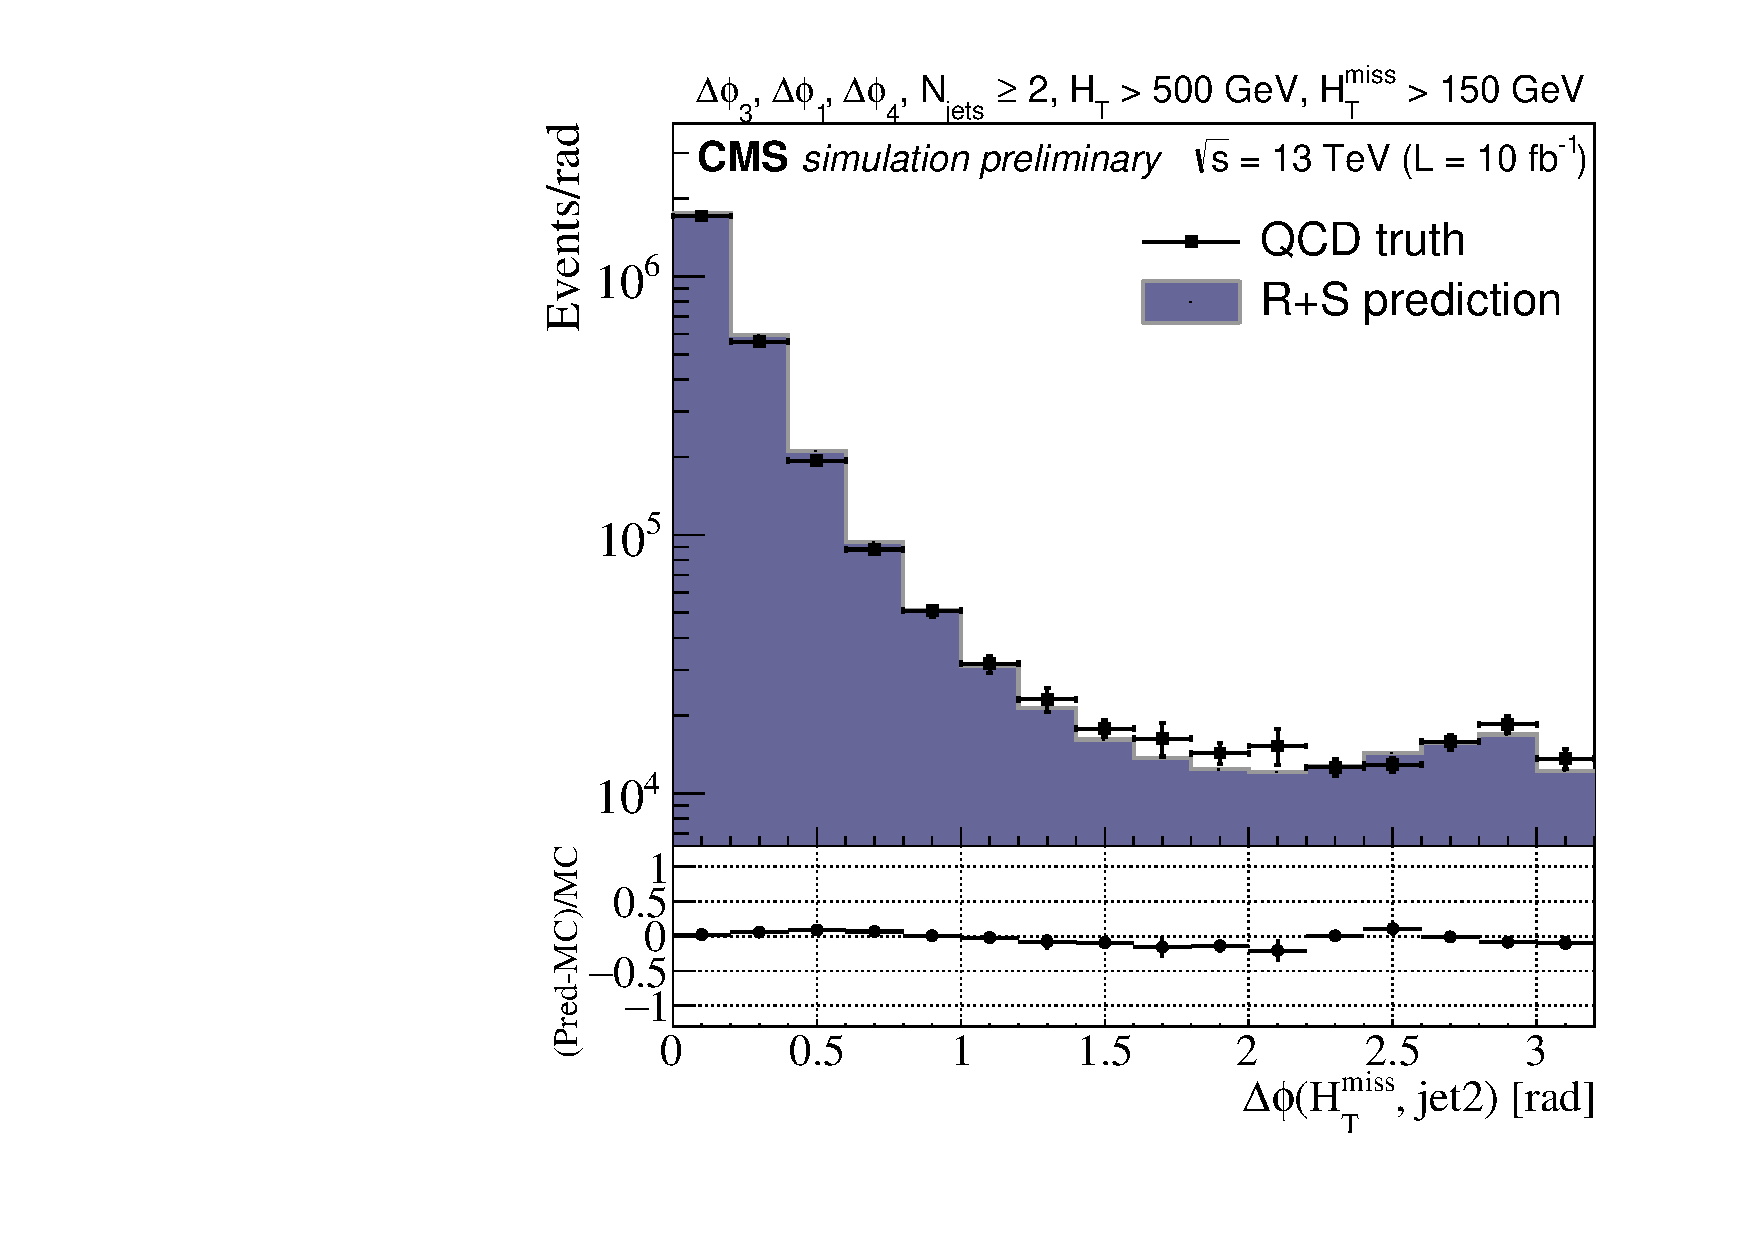
\includegraphics[width=0.5\linewidth]{figures/SusySearches/Ra2b2016/Baseline_DPhi2.pdf}
}\\
\subfloat[]{
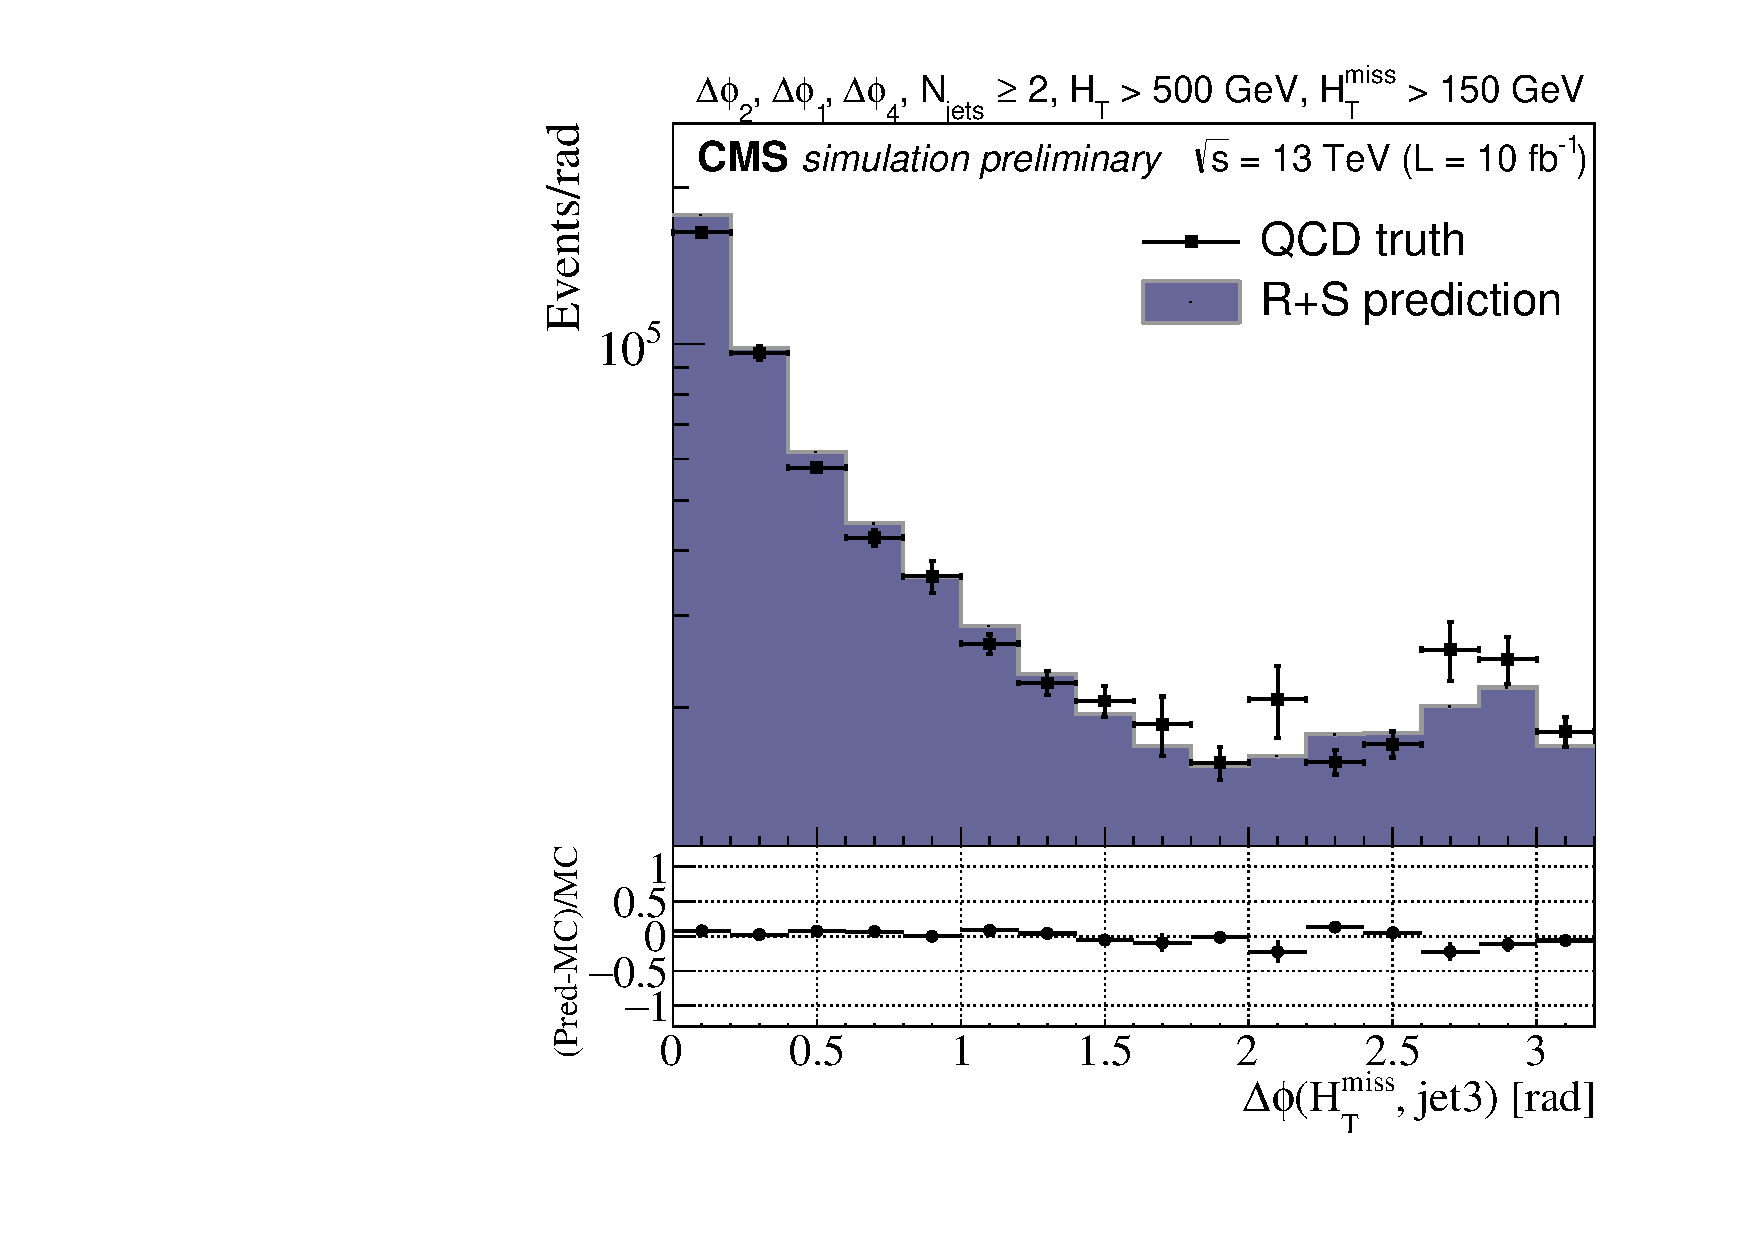
\includegraphics[width=0.5\linewidth]{figures/SusySearches/Ra2b2016/Baseline_DPhi3.pdf}
}
\subfloat[]{
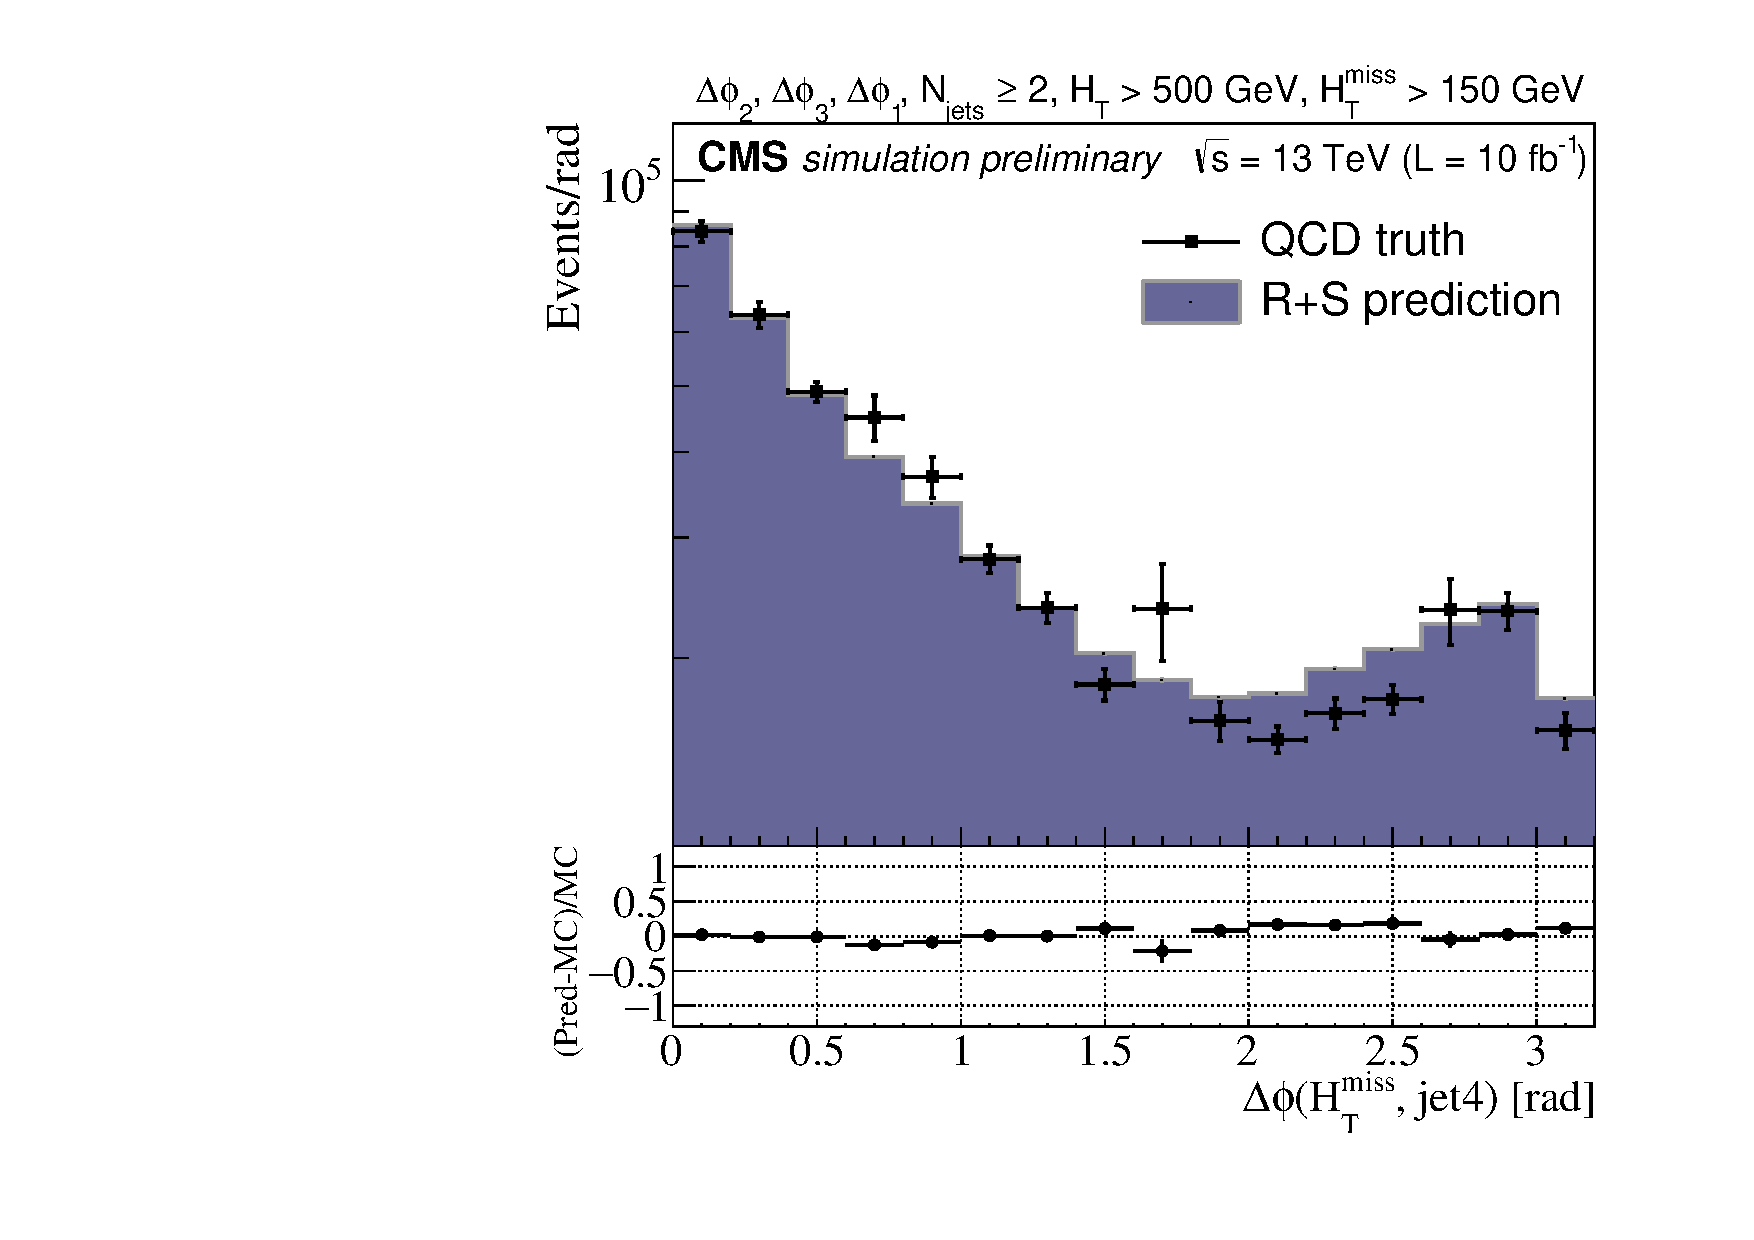
\includegraphics[width=0.5\linewidth]{figures/SusySearches/Ra2b2016/Baseline_DPhi4.pdf}
}
\caption{Comparisons of kinematic distributions between the direct simulation and the rebalance and smear method applied to simulation, after the baseline selection of the multi-jet SUSY search.}
\label{fig:BaselineRplusS2}
\end{figure}

\begin{figure}[h]
\centering
\subfloat[]{
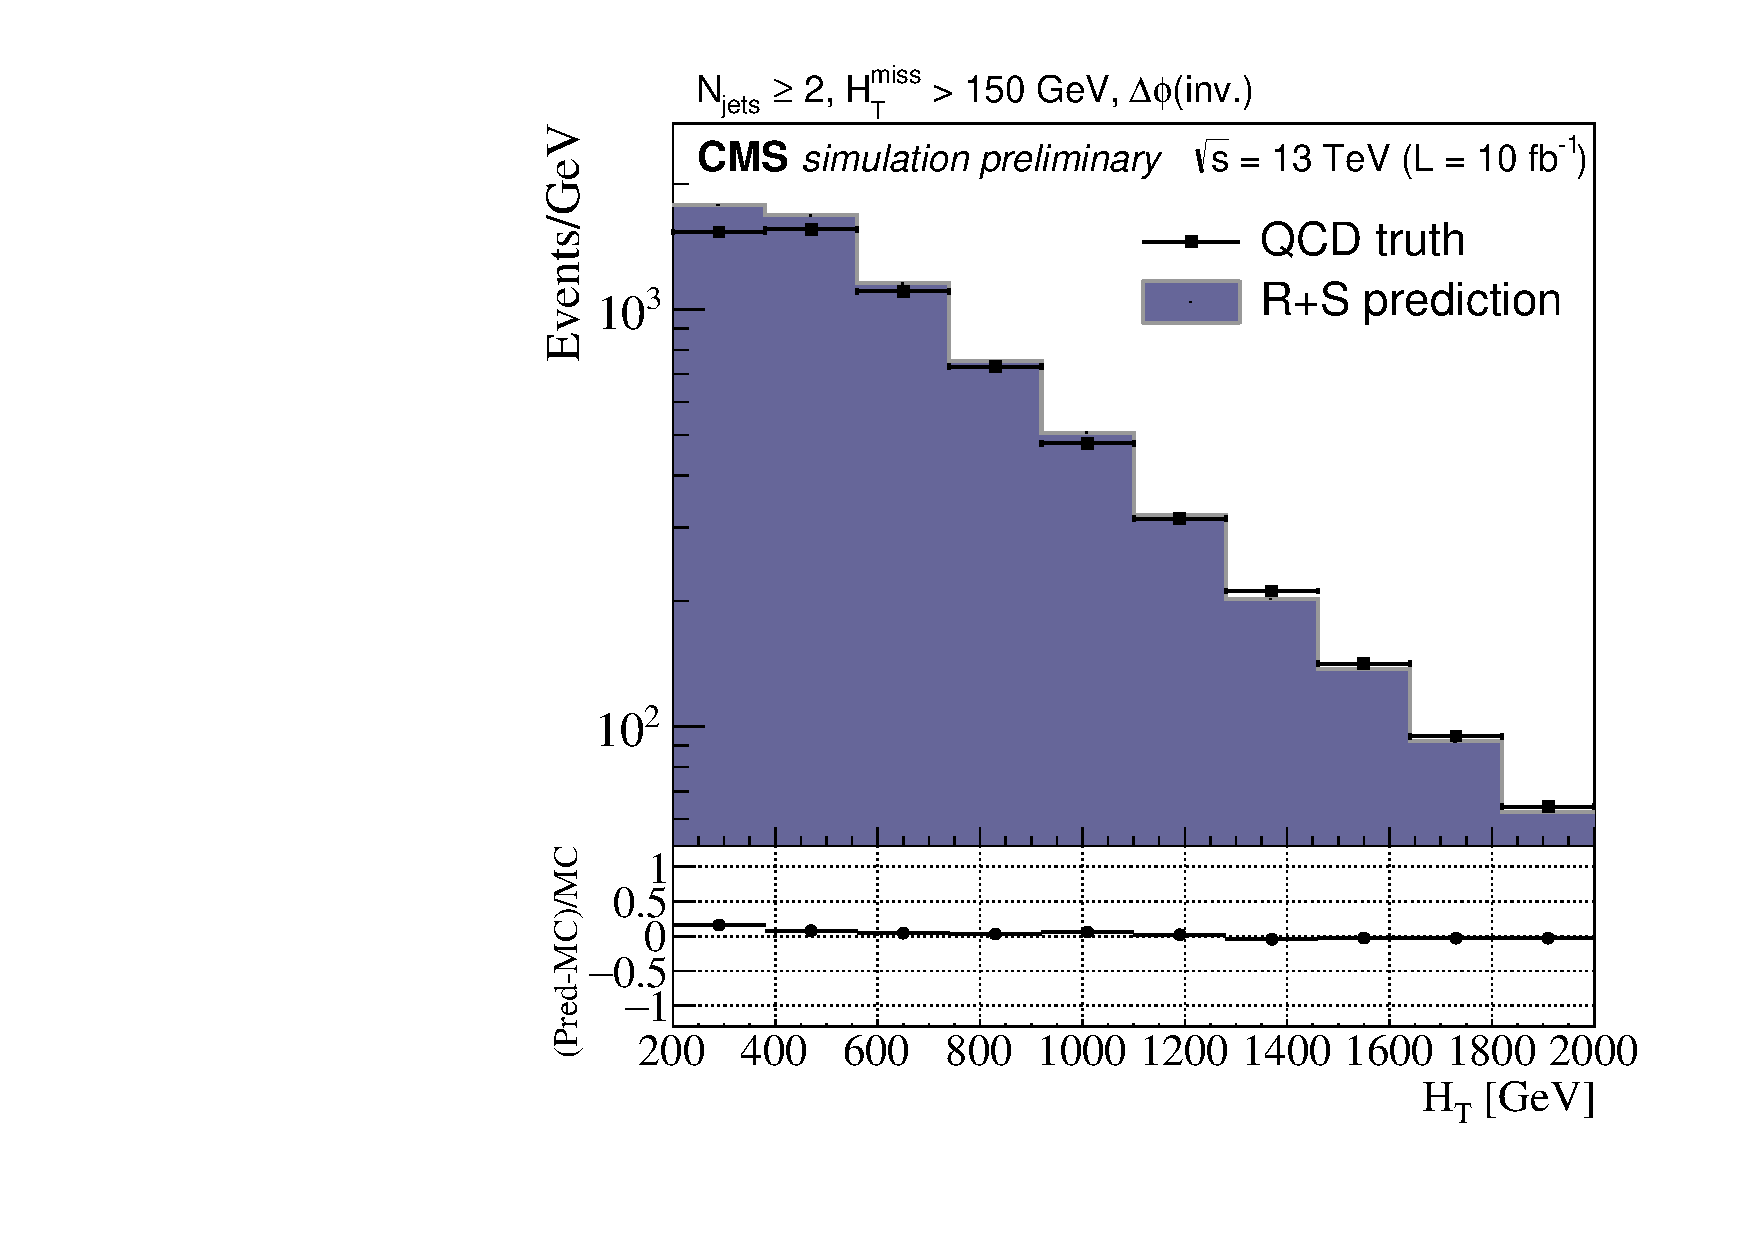
\includegraphics[width=0.5\linewidth]{figures/SusySearches/Ra2b2016/LowDeltaPhi_Ht.pdf}
}
\subfloat[]{
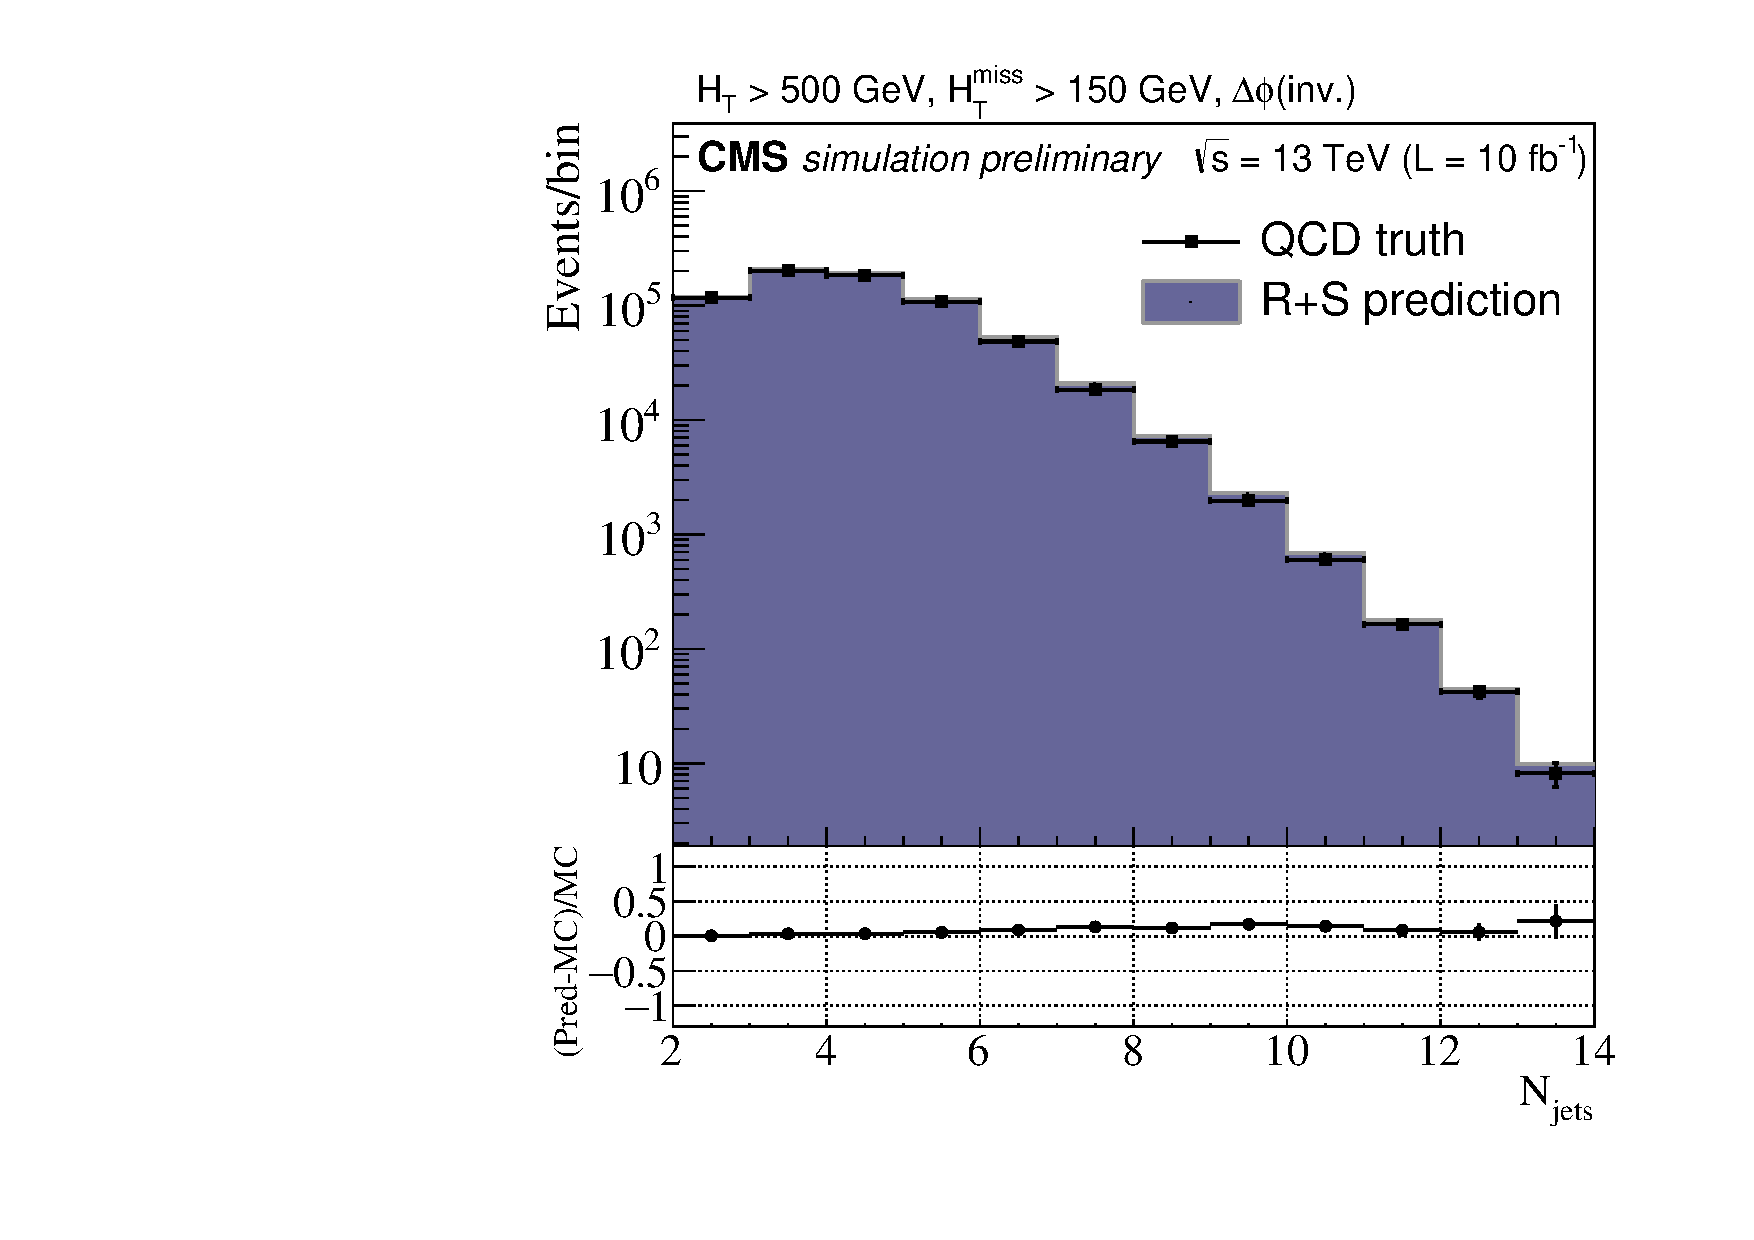
\includegraphics[width=0.5\linewidth]{figures/SusySearches/Ra2b2016/LowDeltaPhi_NJets.pdf}
}\\
\subfloat[]{
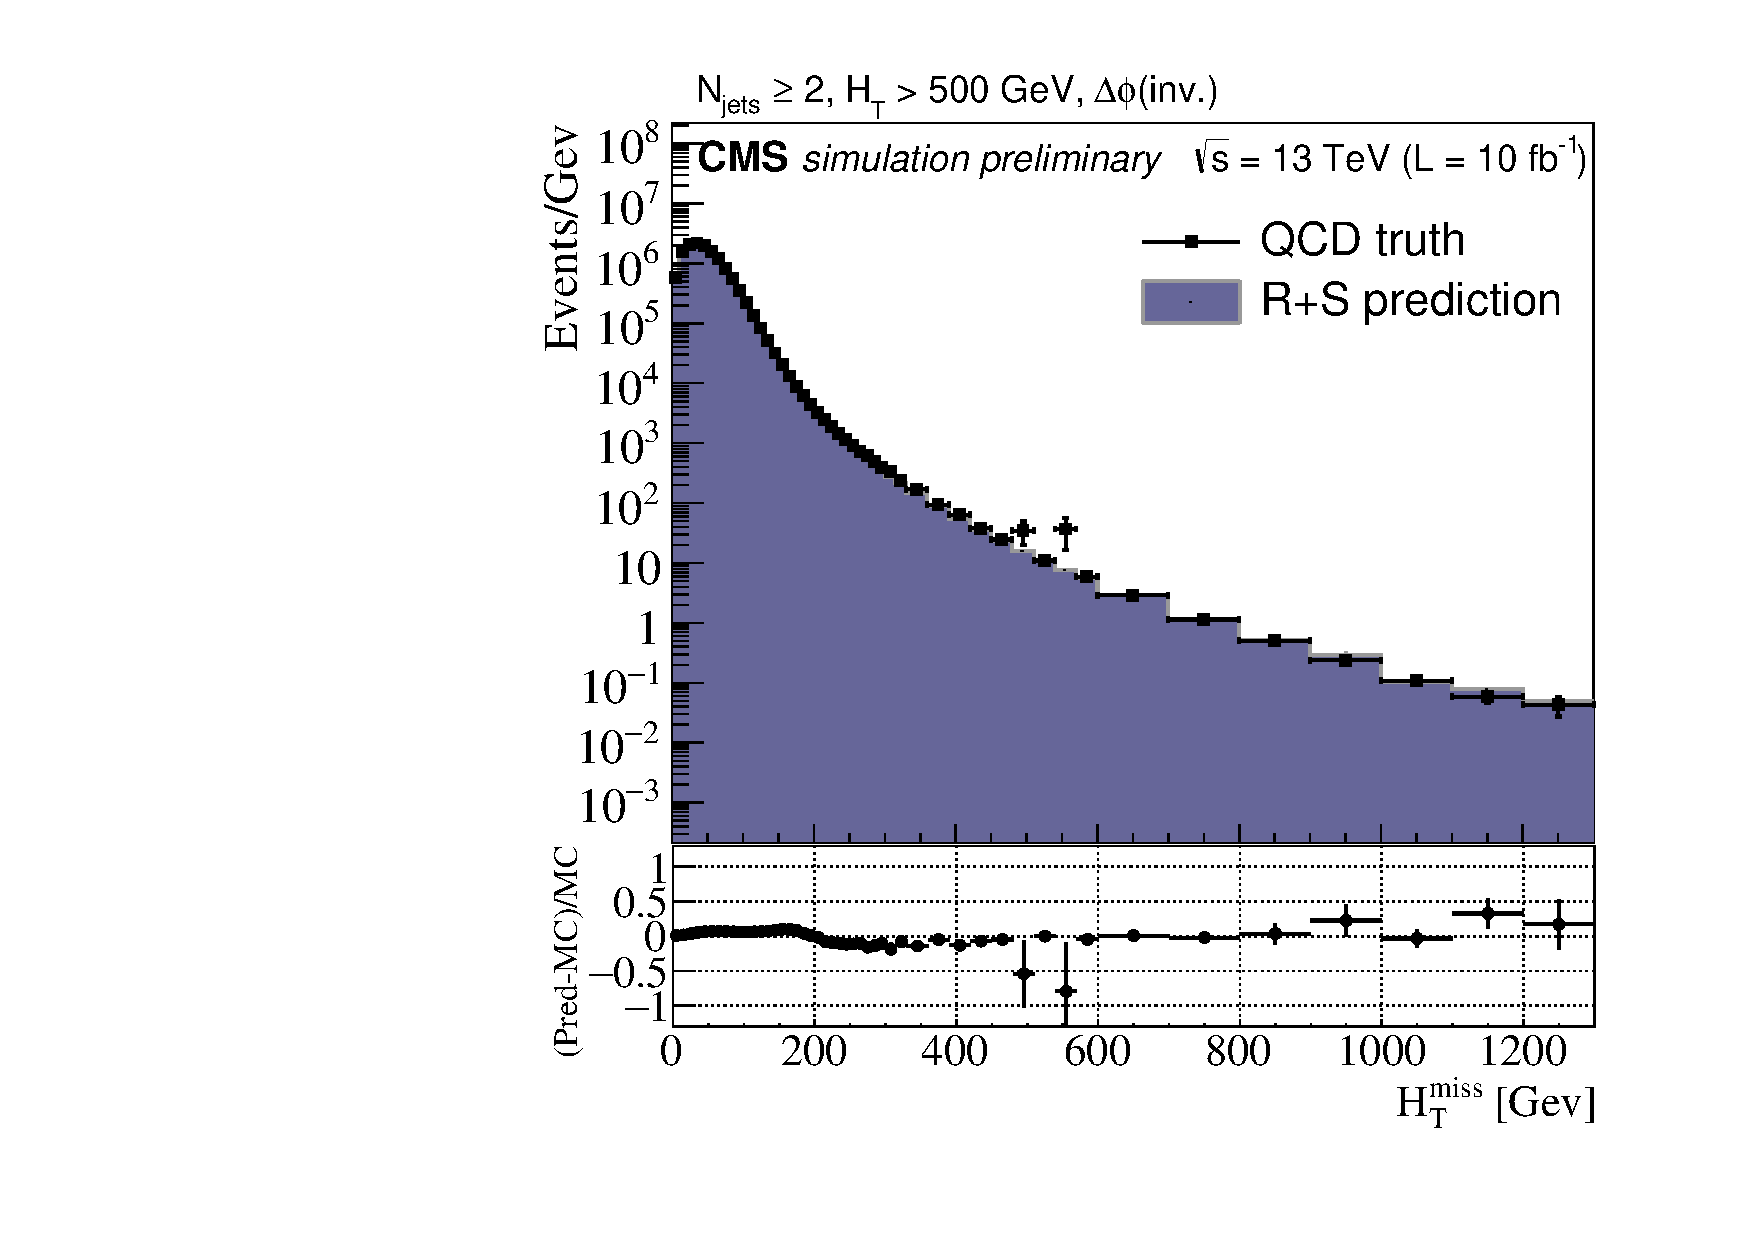
\includegraphics[width=0.5\linewidth]{figures/SusySearches/Ra2b2016/LowDeltaPhi_Mht.pdf}
}
\subfloat[]{
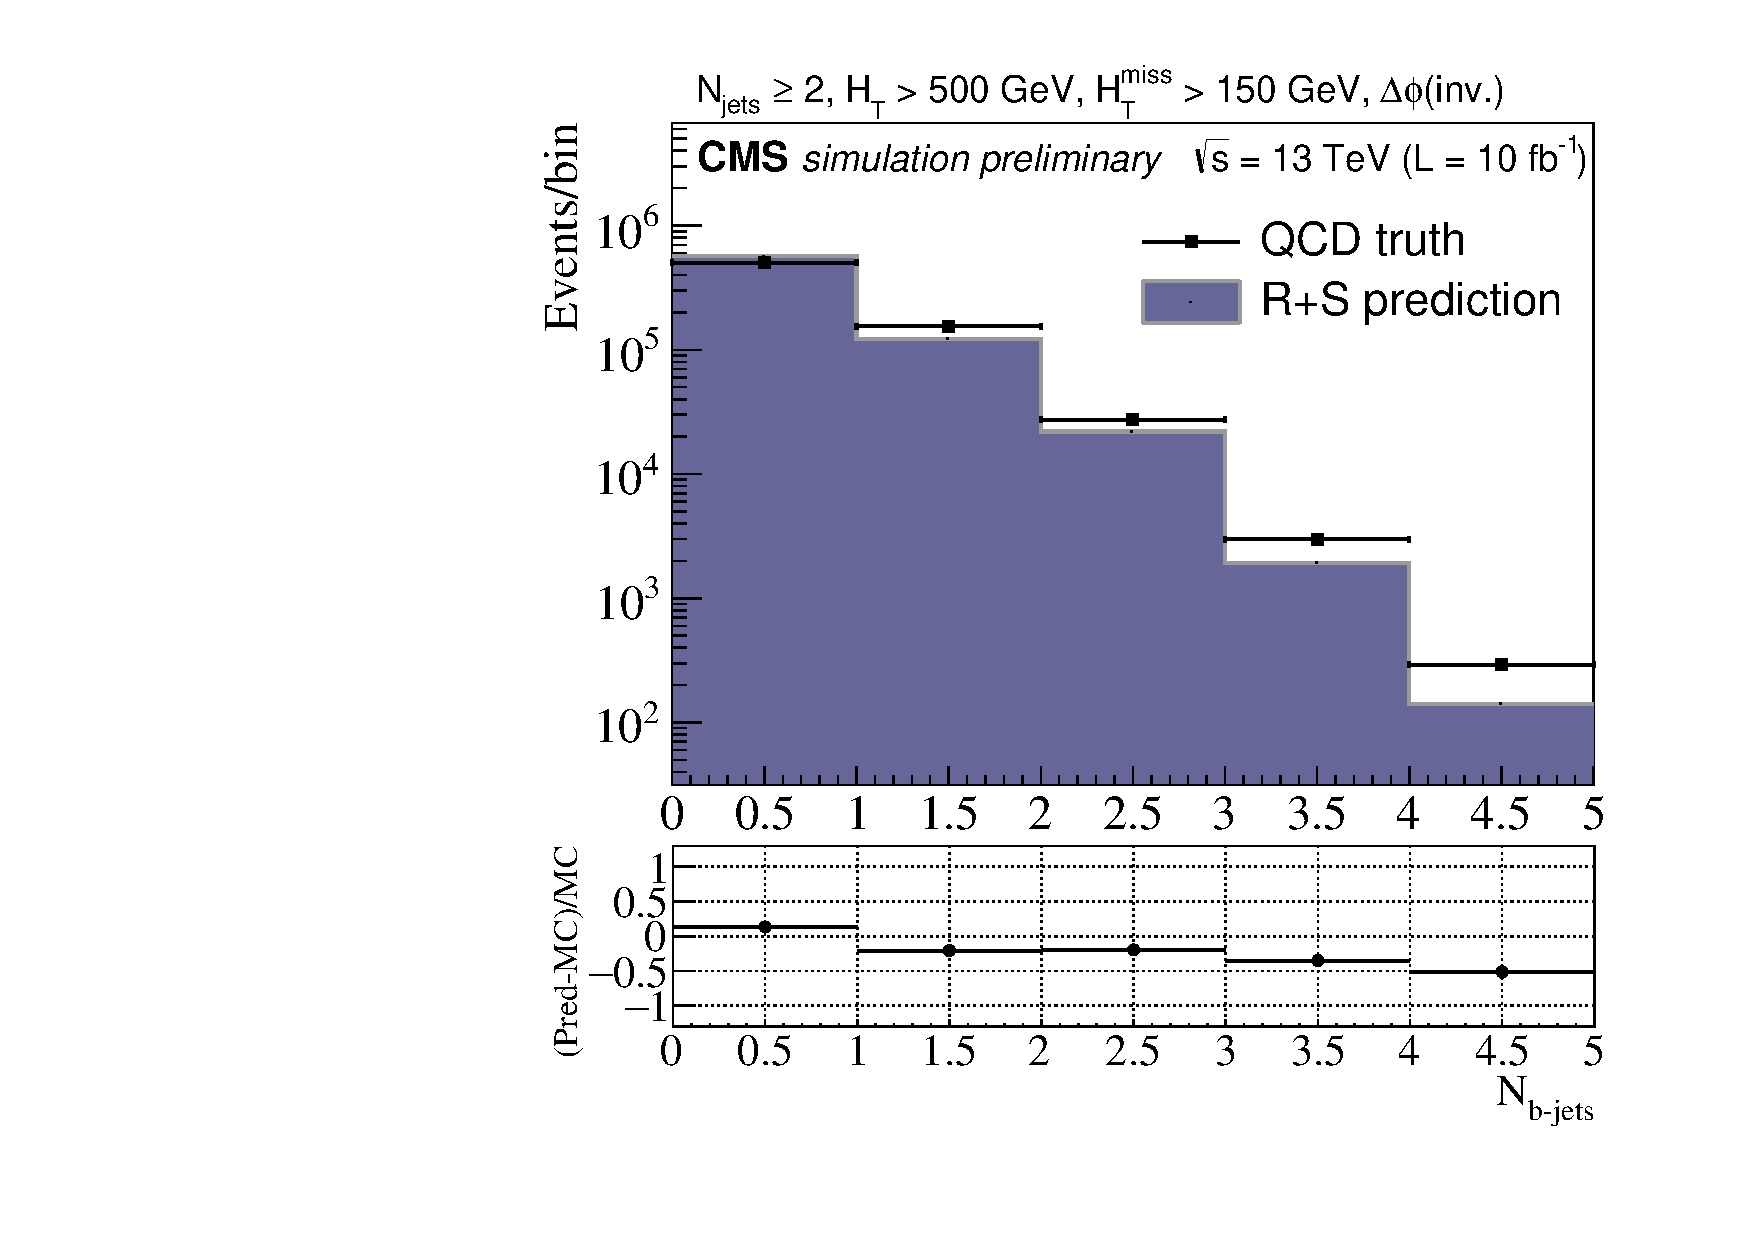
\includegraphics[width=0.5\linewidth]{figures/SusySearches/Ra2b2016/LowDeltaPhi_BTags.pdf}
}
\caption{Comparisons of kinematic distributions between the direct simulation and the rebalance and smear method applied to simulation, in the inverted $\Delta \phi$ control region of the multi-jet SUSY search.}
\label{fig:LowDeltaPhiRplusS}
\end{figure}

\begin{figure}[h]
\centering
\subfloat[]{
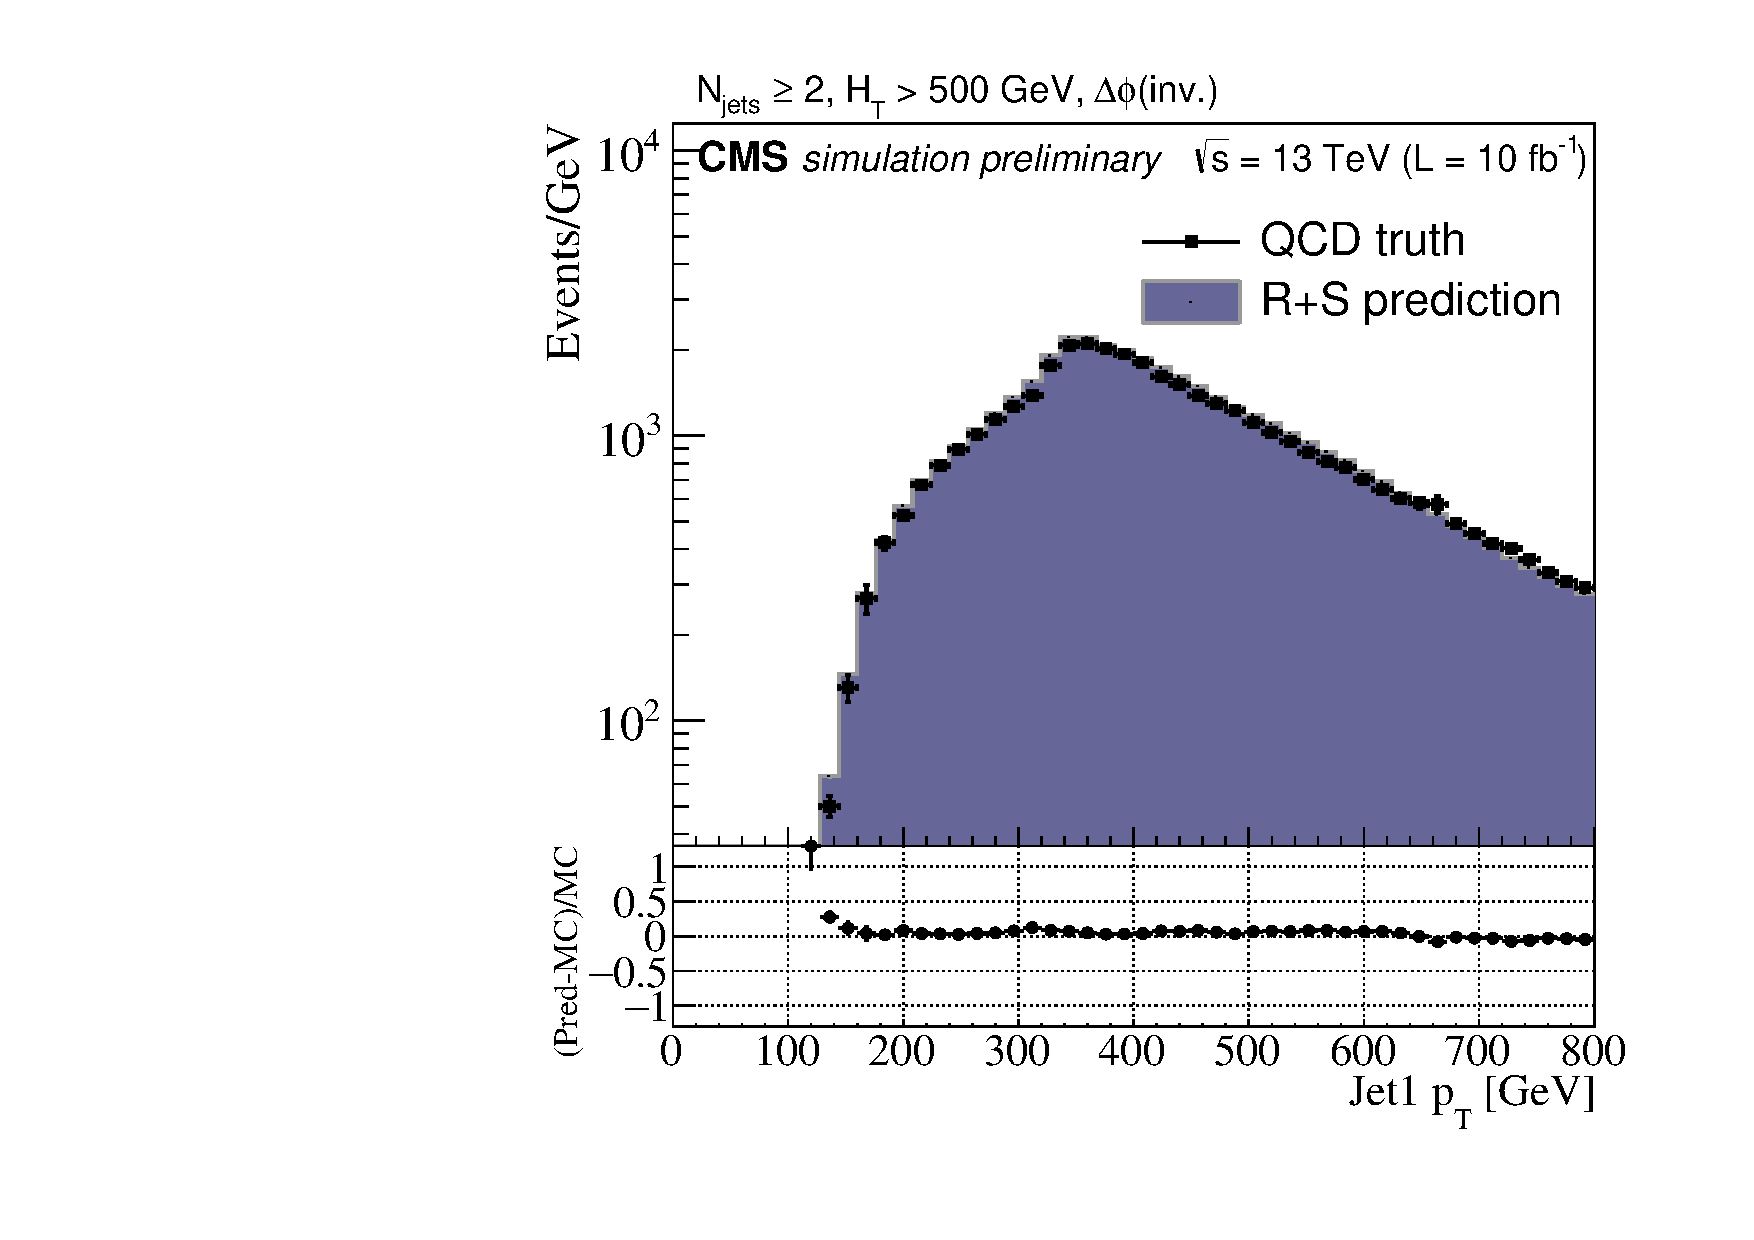
\includegraphics[width=0.5\linewidth]{figures/SusySearches/Ra2b2016/LowDeltaPhi_Jet1Pt.pdf}
}
\subfloat[]{
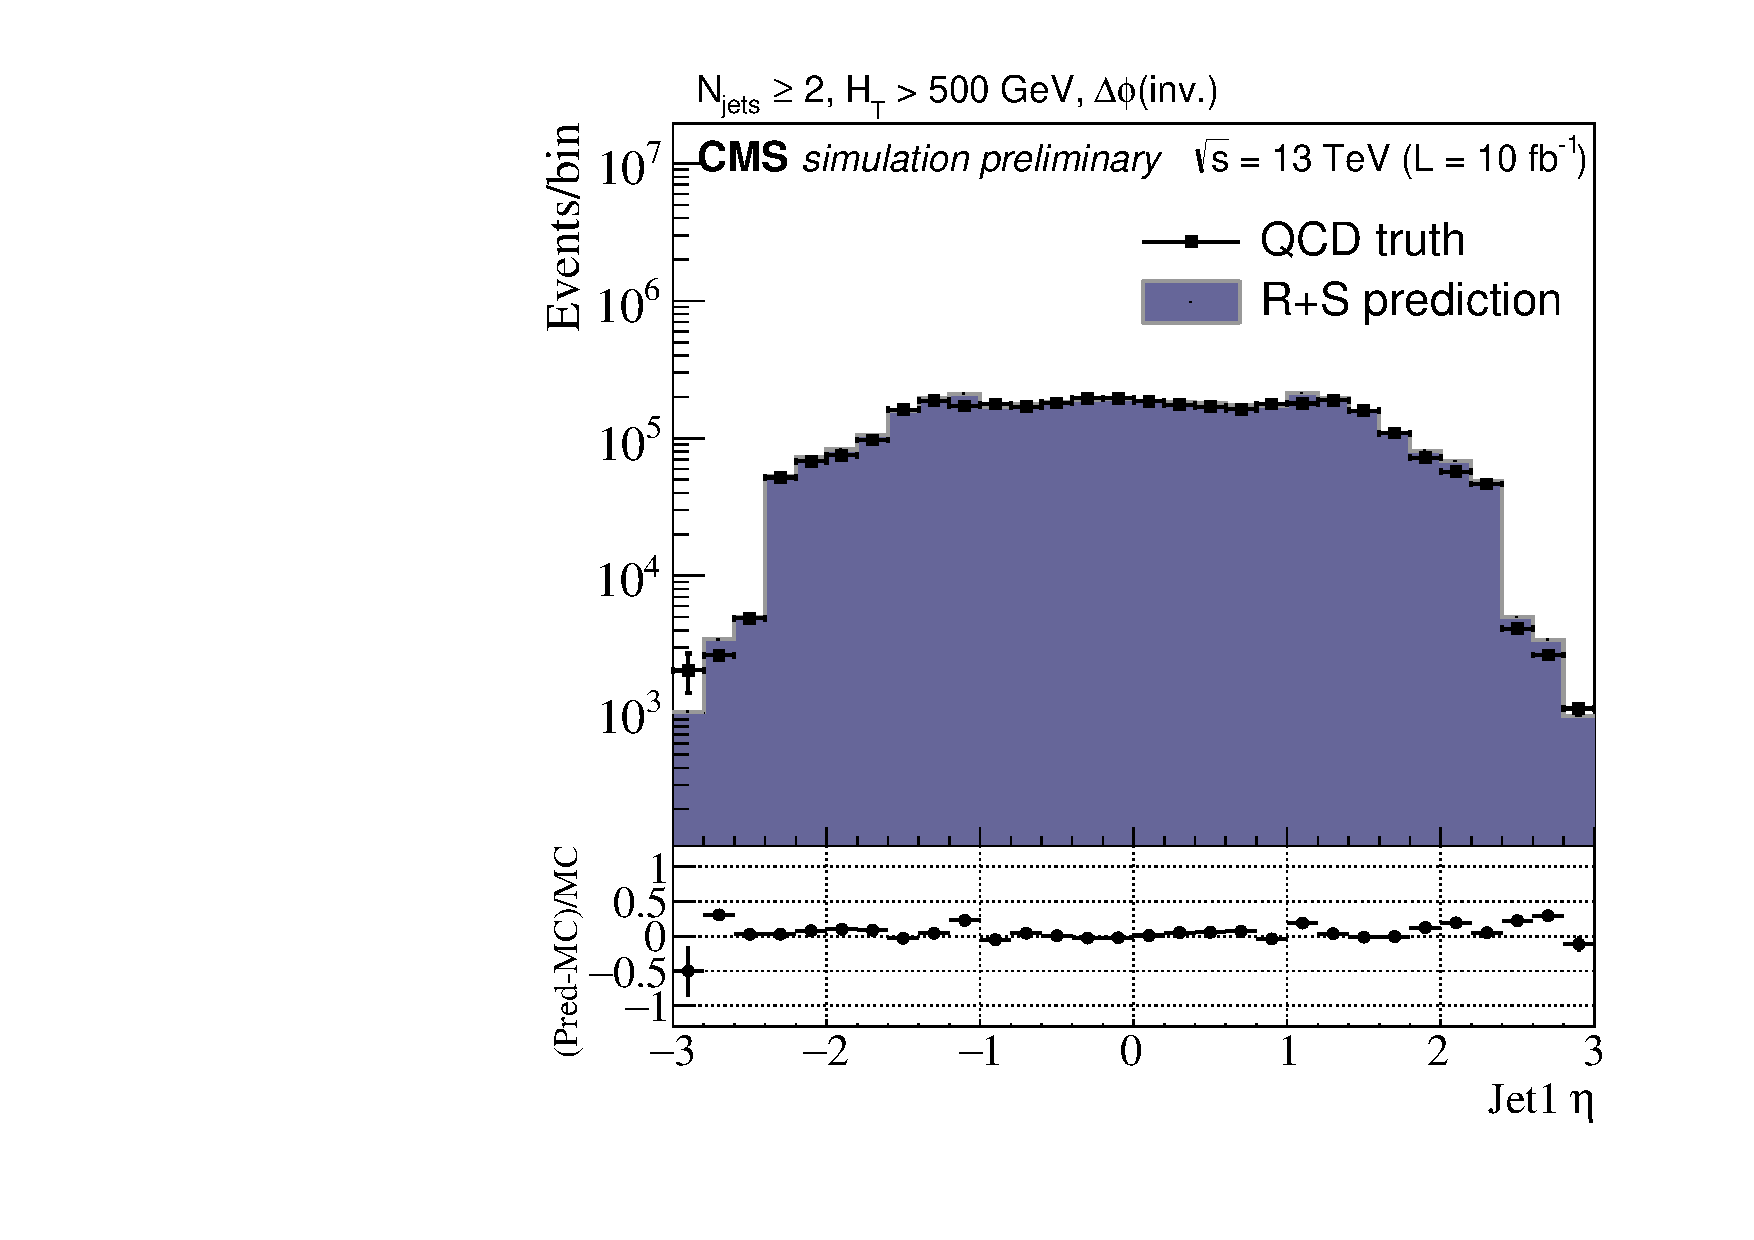
\includegraphics[width=0.5\linewidth]{figures/SusySearches/Ra2b2016/LowDeltaPhi_Jet1Eta.pdf}
}\\
\subfloat[]{
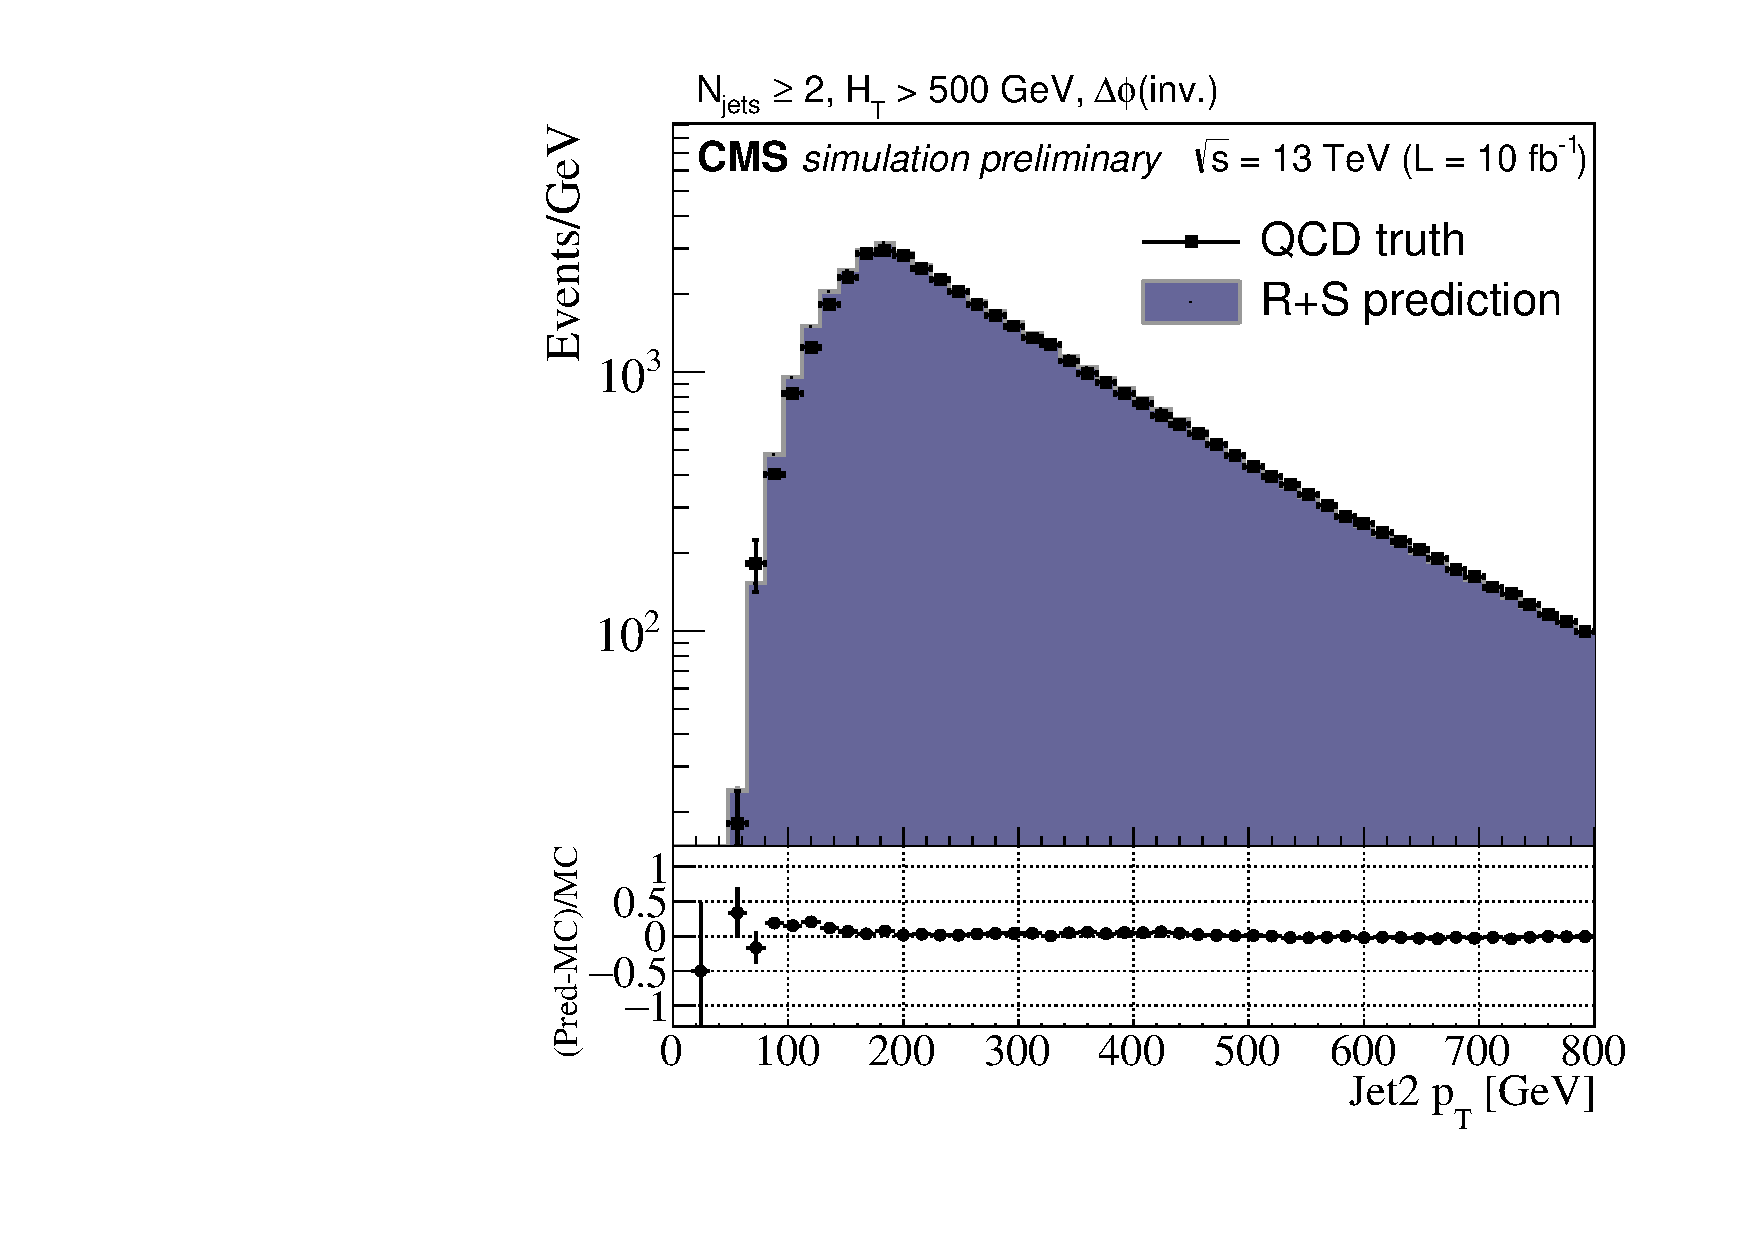
\includegraphics[width=0.5\linewidth]{figures/SusySearches/Ra2b2016/LowDeltaPhi_Jet2Pt.pdf}
}
\subfloat[]{
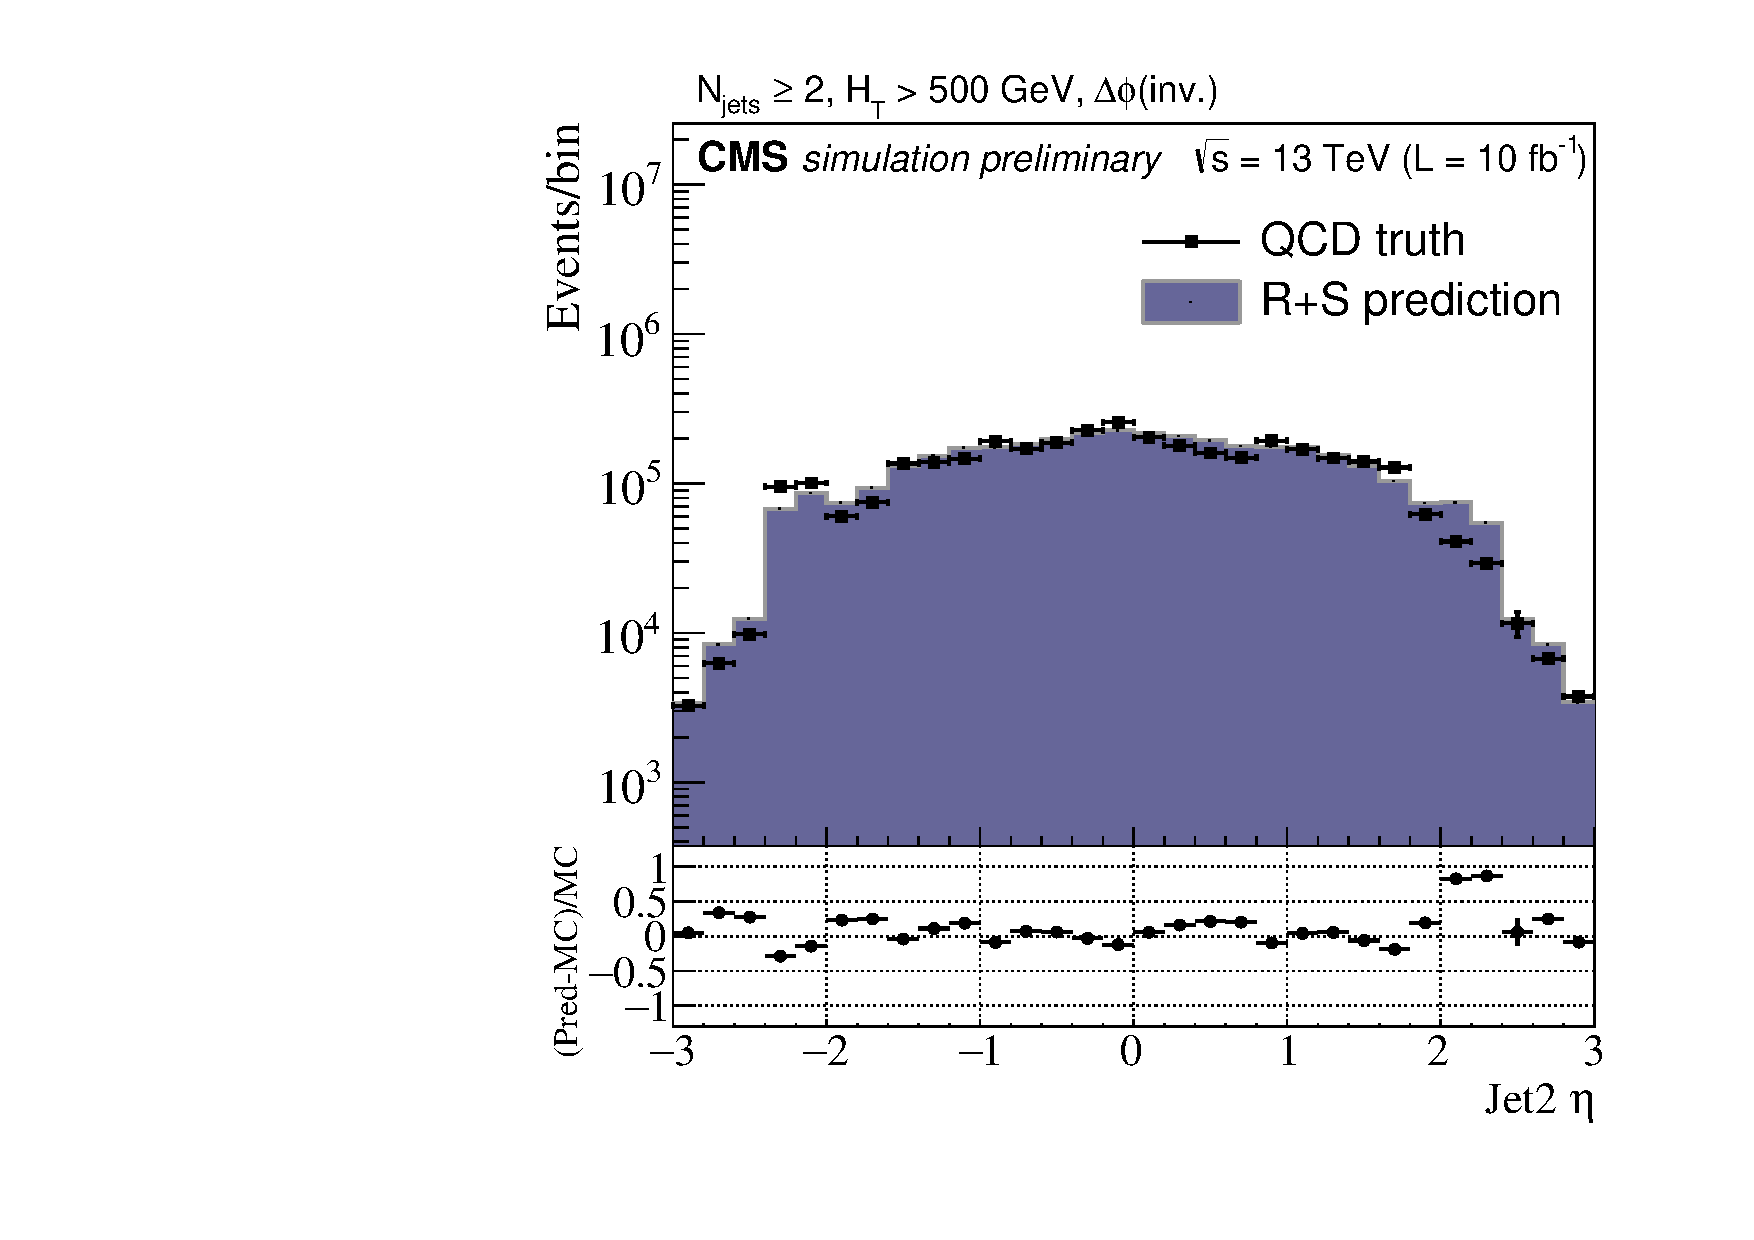
\includegraphics[width=0.5\linewidth]{figures/SusySearches/Ra2b2016/LowDeltaPhi_Jet2Eta.pdf}
}
\caption{Comparisons of kinematic distributions between the direct simulation and the rebalance and smear method applied to simulation, in the inverted $\Delta \phi$ control region of the multi-jet SUSY search.}
\label{fig:LowDeltaPhiRplusSb}
\end{figure}

\begin{figure}[h]
\centering
\subfloat[]{
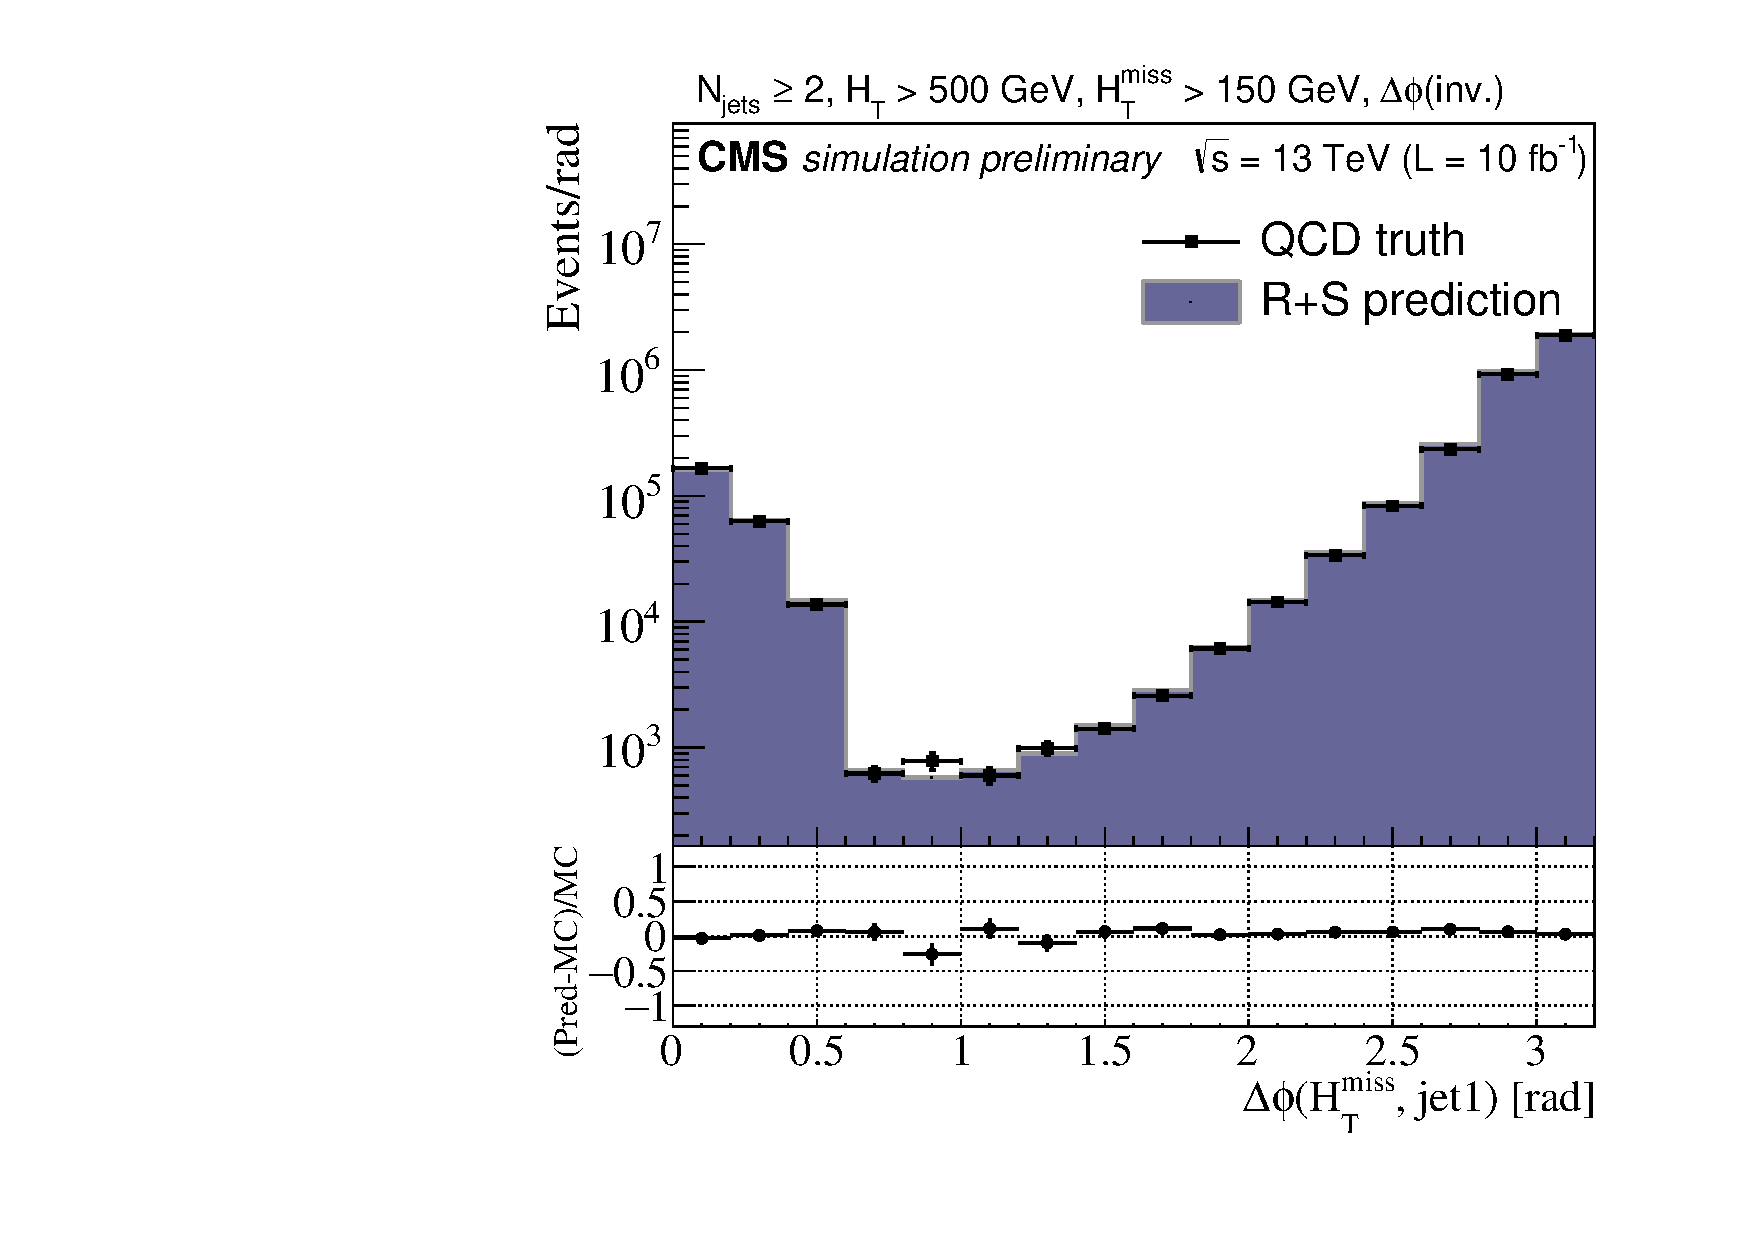
\includegraphics[width=0.5\linewidth]{figures/SusySearches/Ra2b2016/LowDeltaPhi_DPhi1.pdf}
}
\subfloat[]{
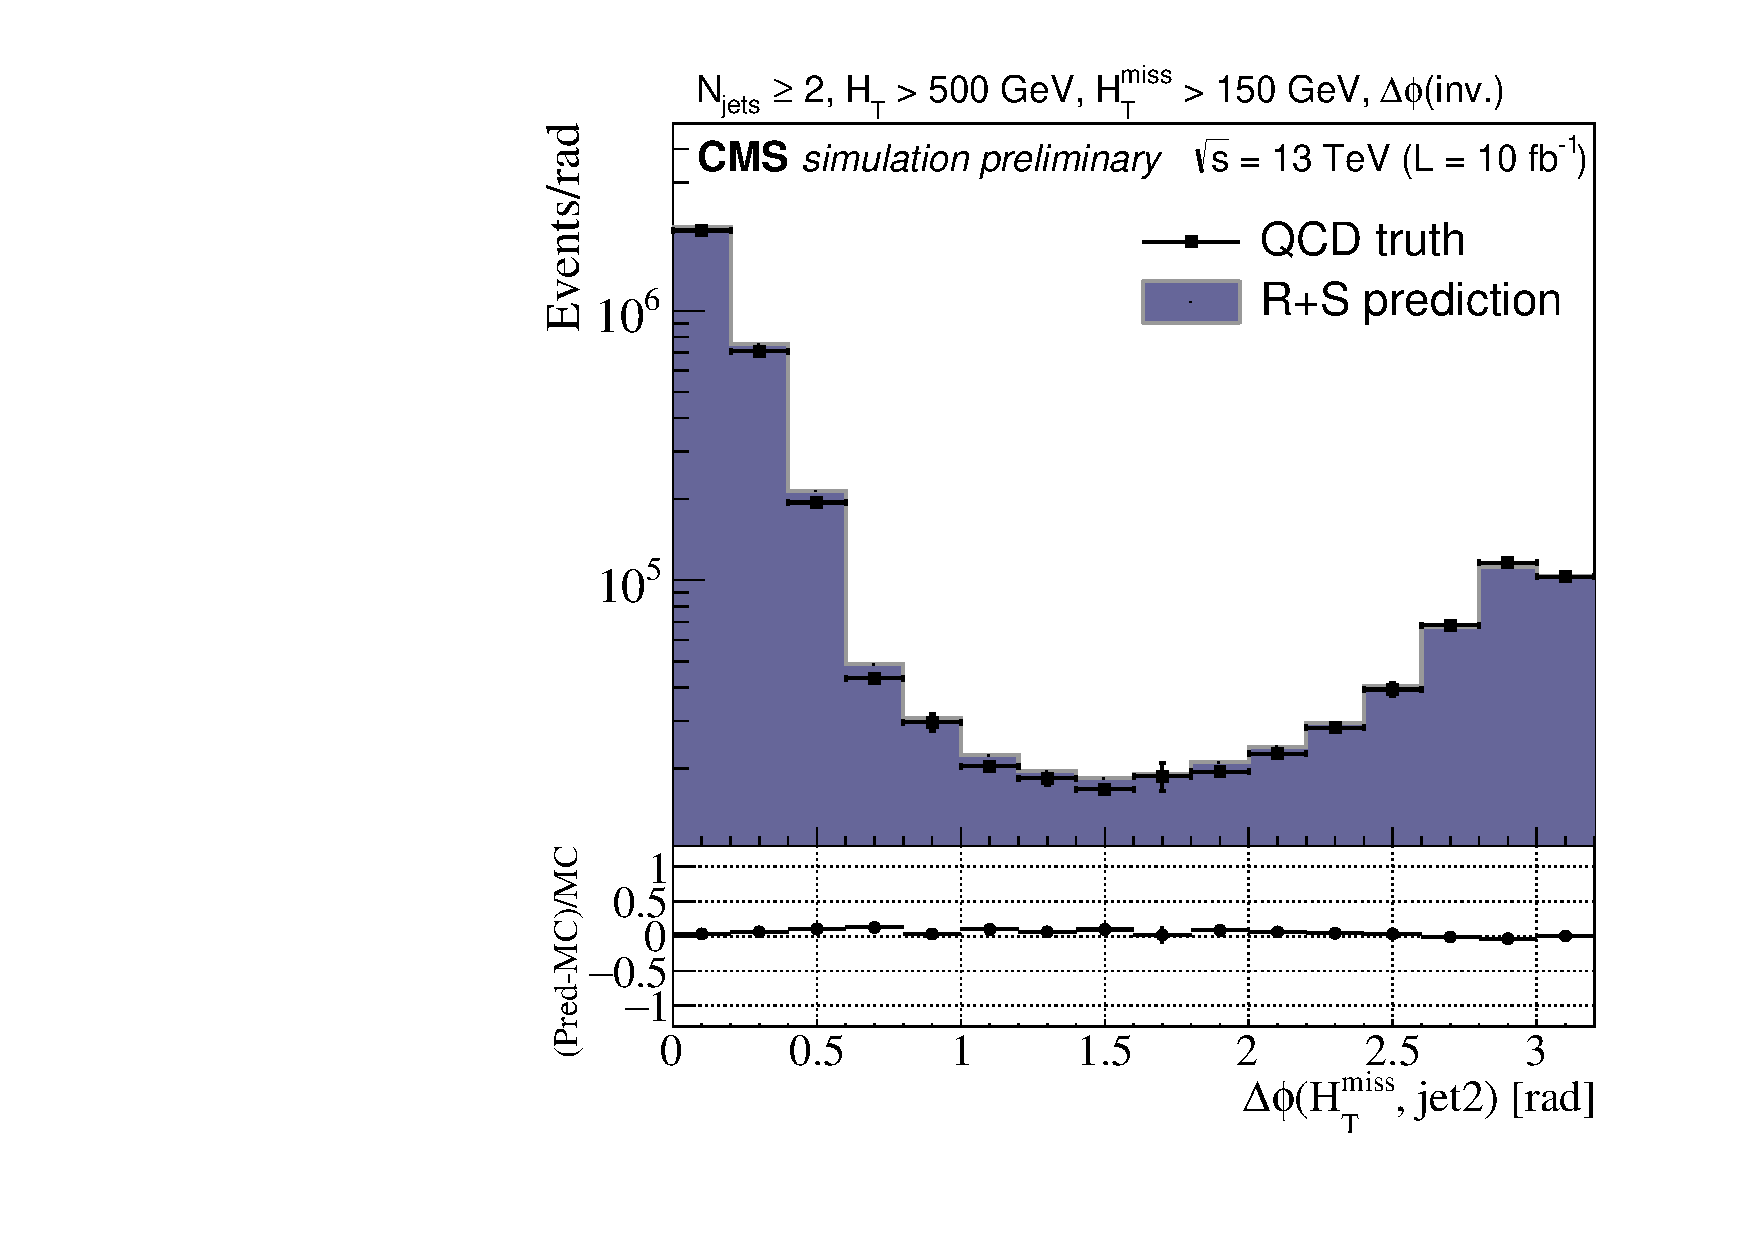
\includegraphics[width=0.5\linewidth]{figures/SusySearches/Ra2b2016/LowDeltaPhi_DPhi2.pdf}
}\\
\subfloat[]{
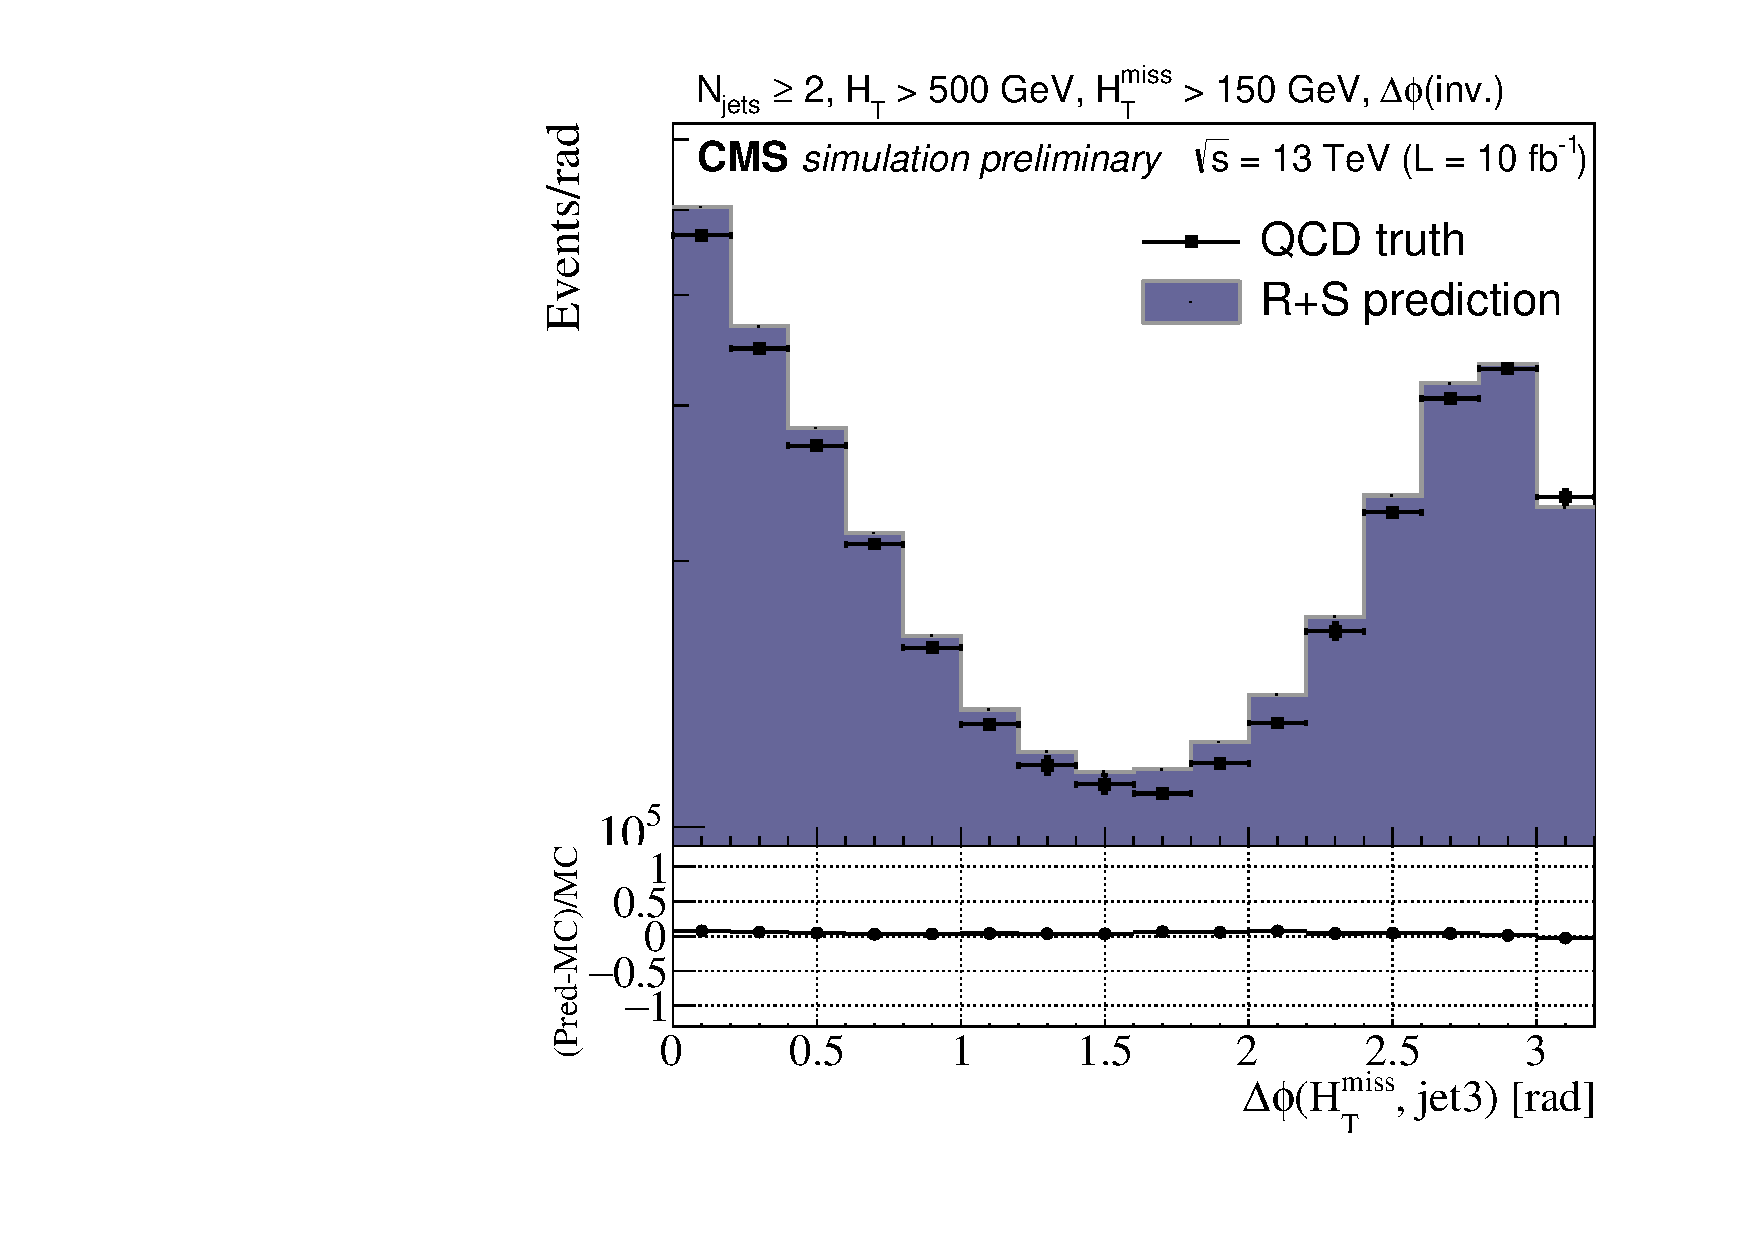
\includegraphics[width=0.5\linewidth]{figures/SusySearches/Ra2b2016/LowDeltaPhi_DPhi3.pdf}
}
\subfloat[]{
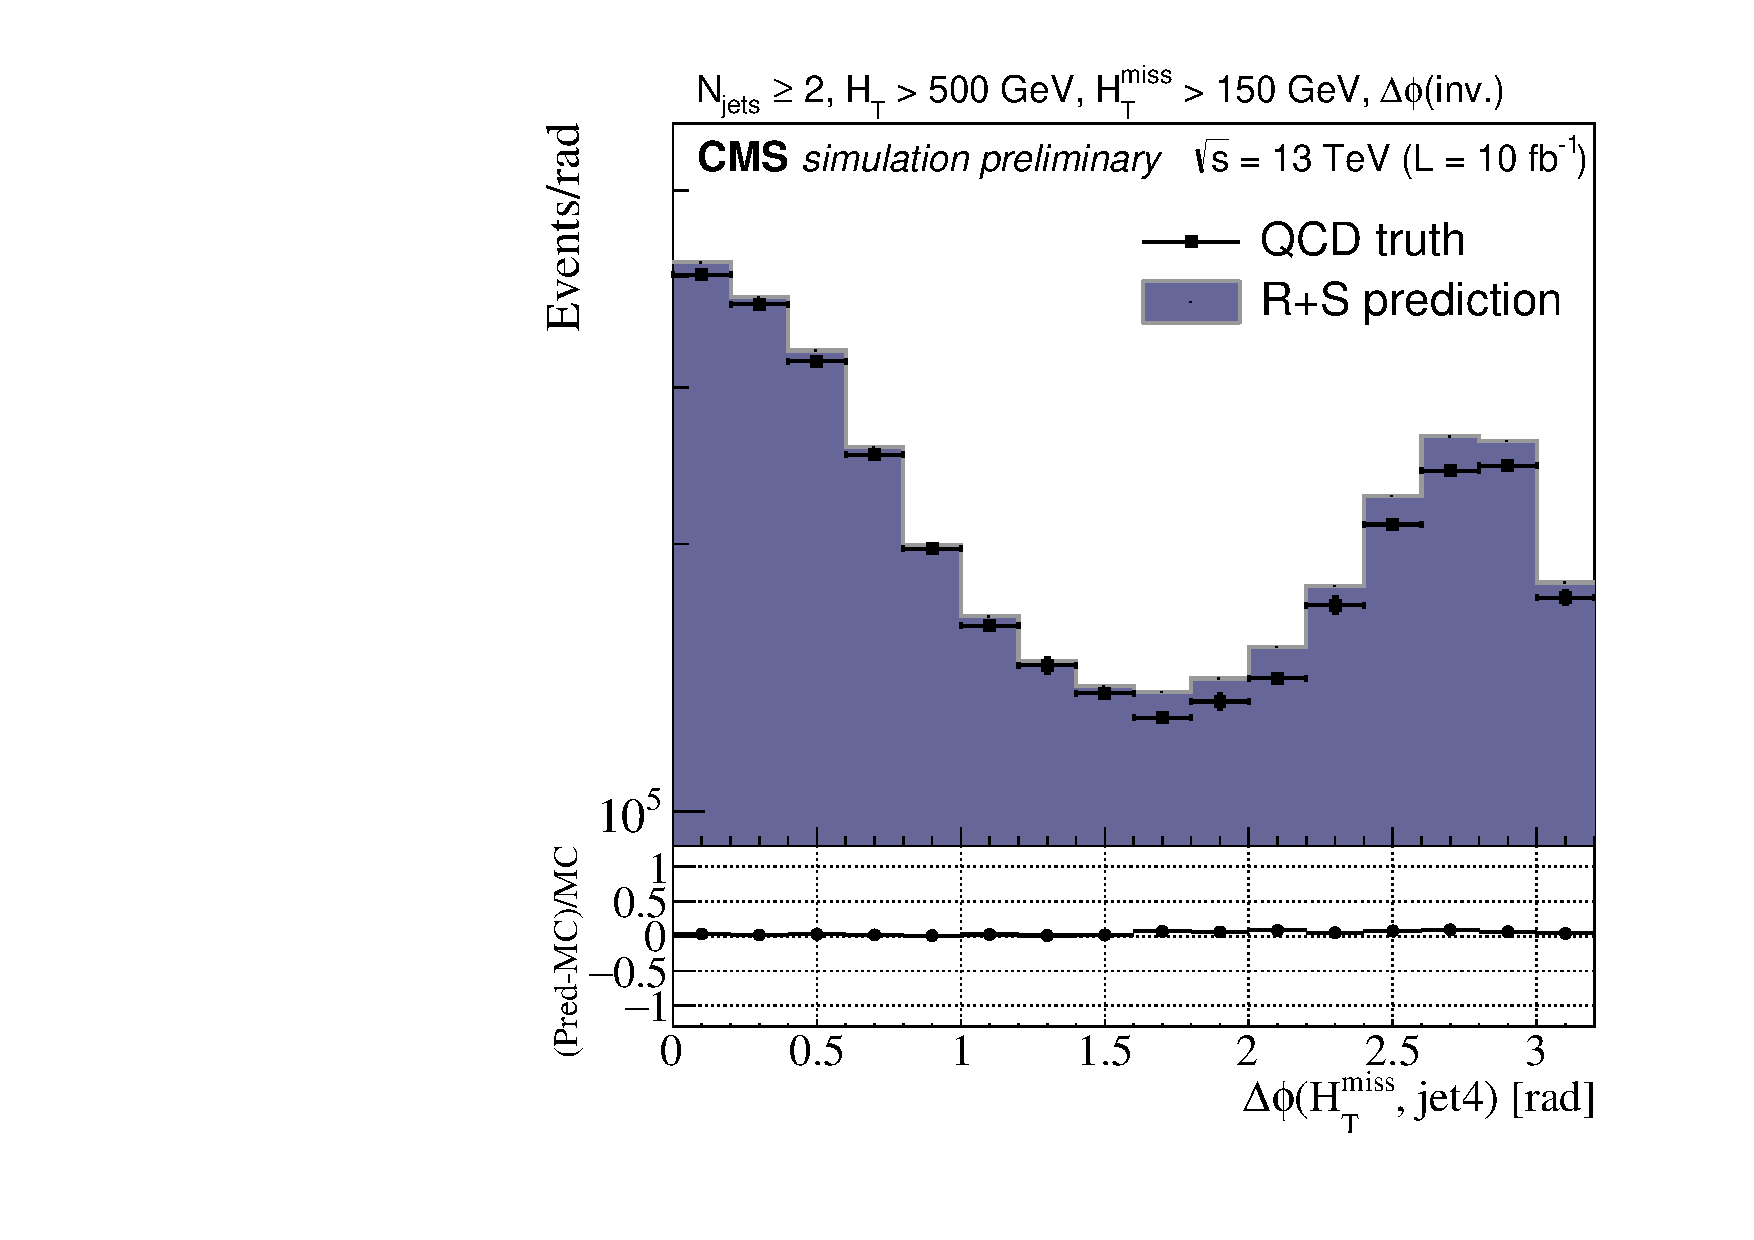
\includegraphics[width=0.5\linewidth]{figures/SusySearches/Ra2b2016/LowDeltaPhi_DPhi4.pdf}
}
\caption{Comparisons of kinematic distributions between the direct simulation and the rebalance and smear method applied to simulation, in the inverted $\Delta \phi$ control region of the multi-jet SUSY search.}
\label{fig:LowDeltaPhiRplusS2}
\end{figure}

\begin{figure}[h]
\centering
\subfloat[]{
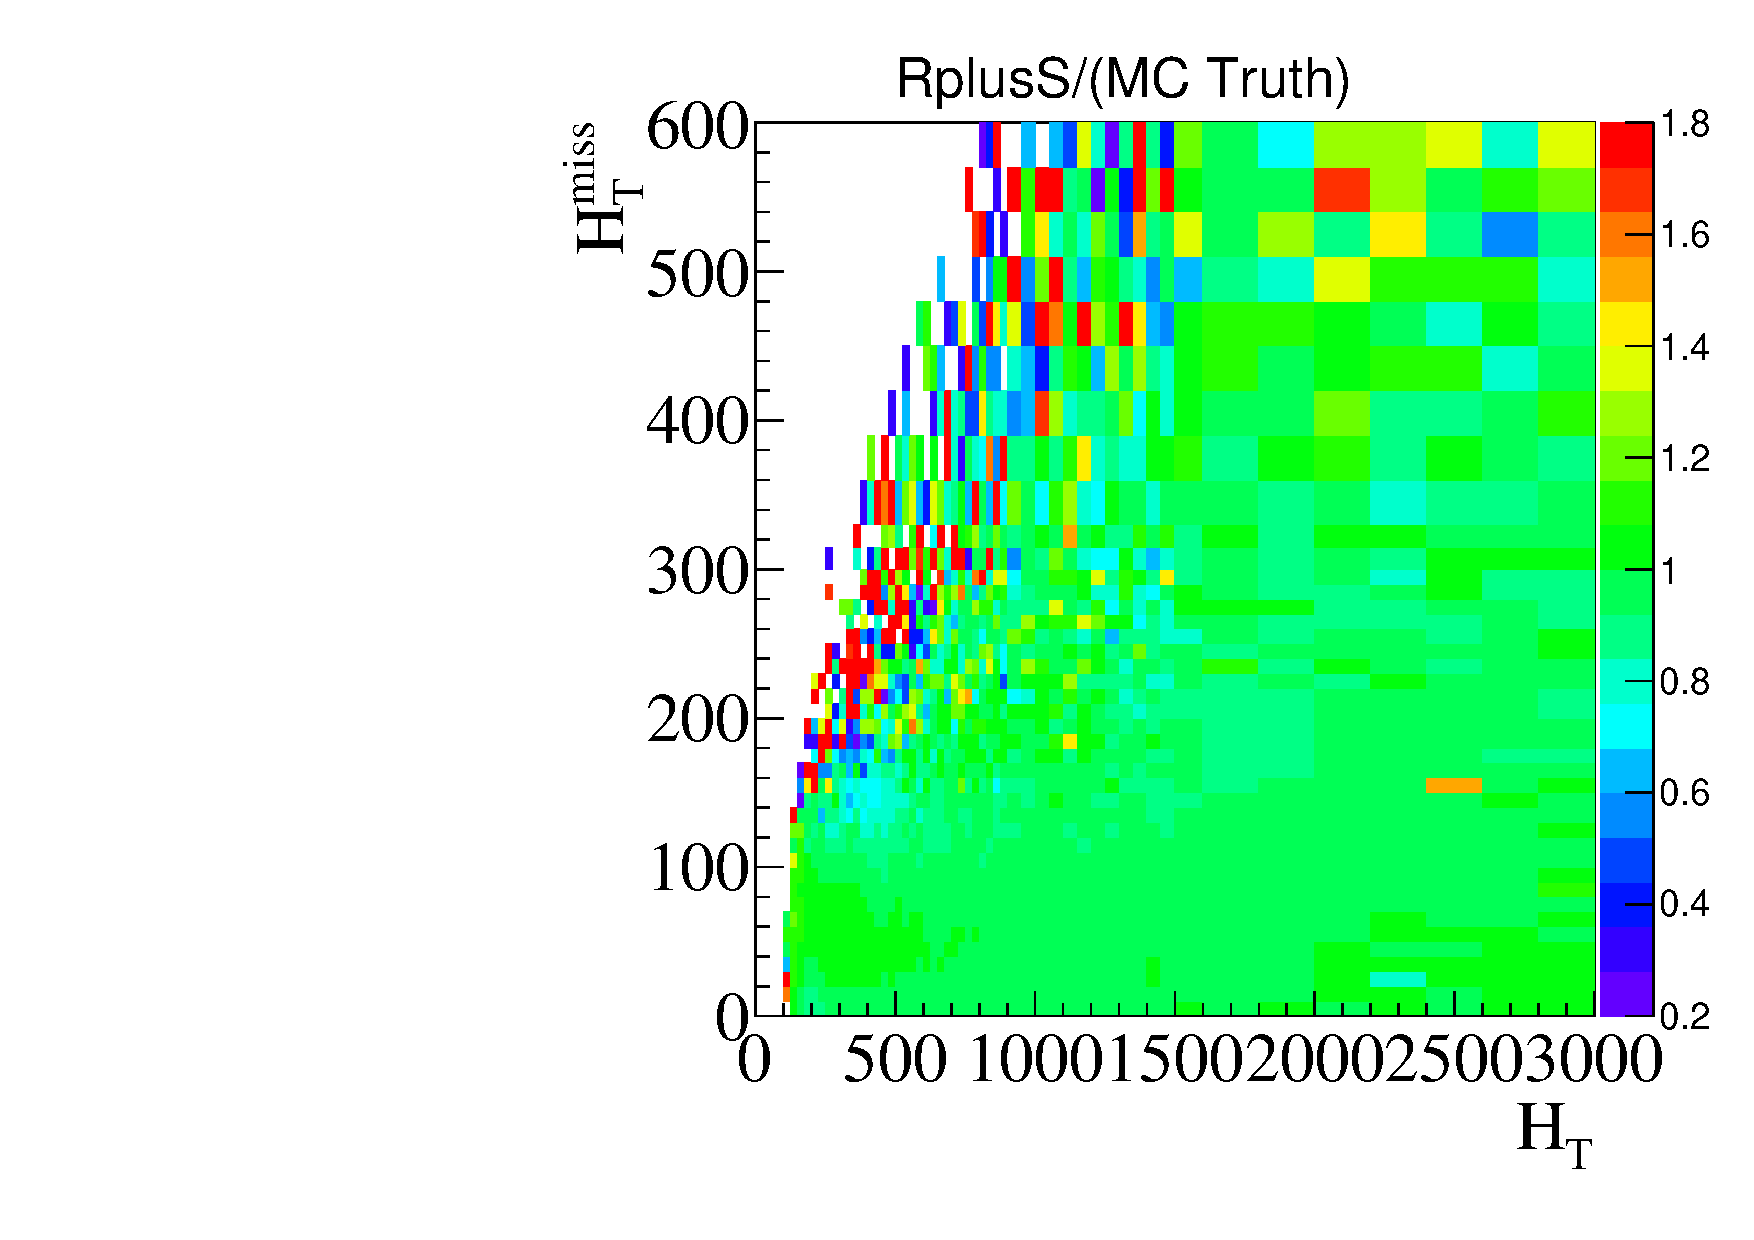
\includegraphics[width=0.5\linewidth]{figures/SusySearches/Ra2b2016/RplusSAndTruth_MhtVsHt.pdf}
}
\subfloat[]{
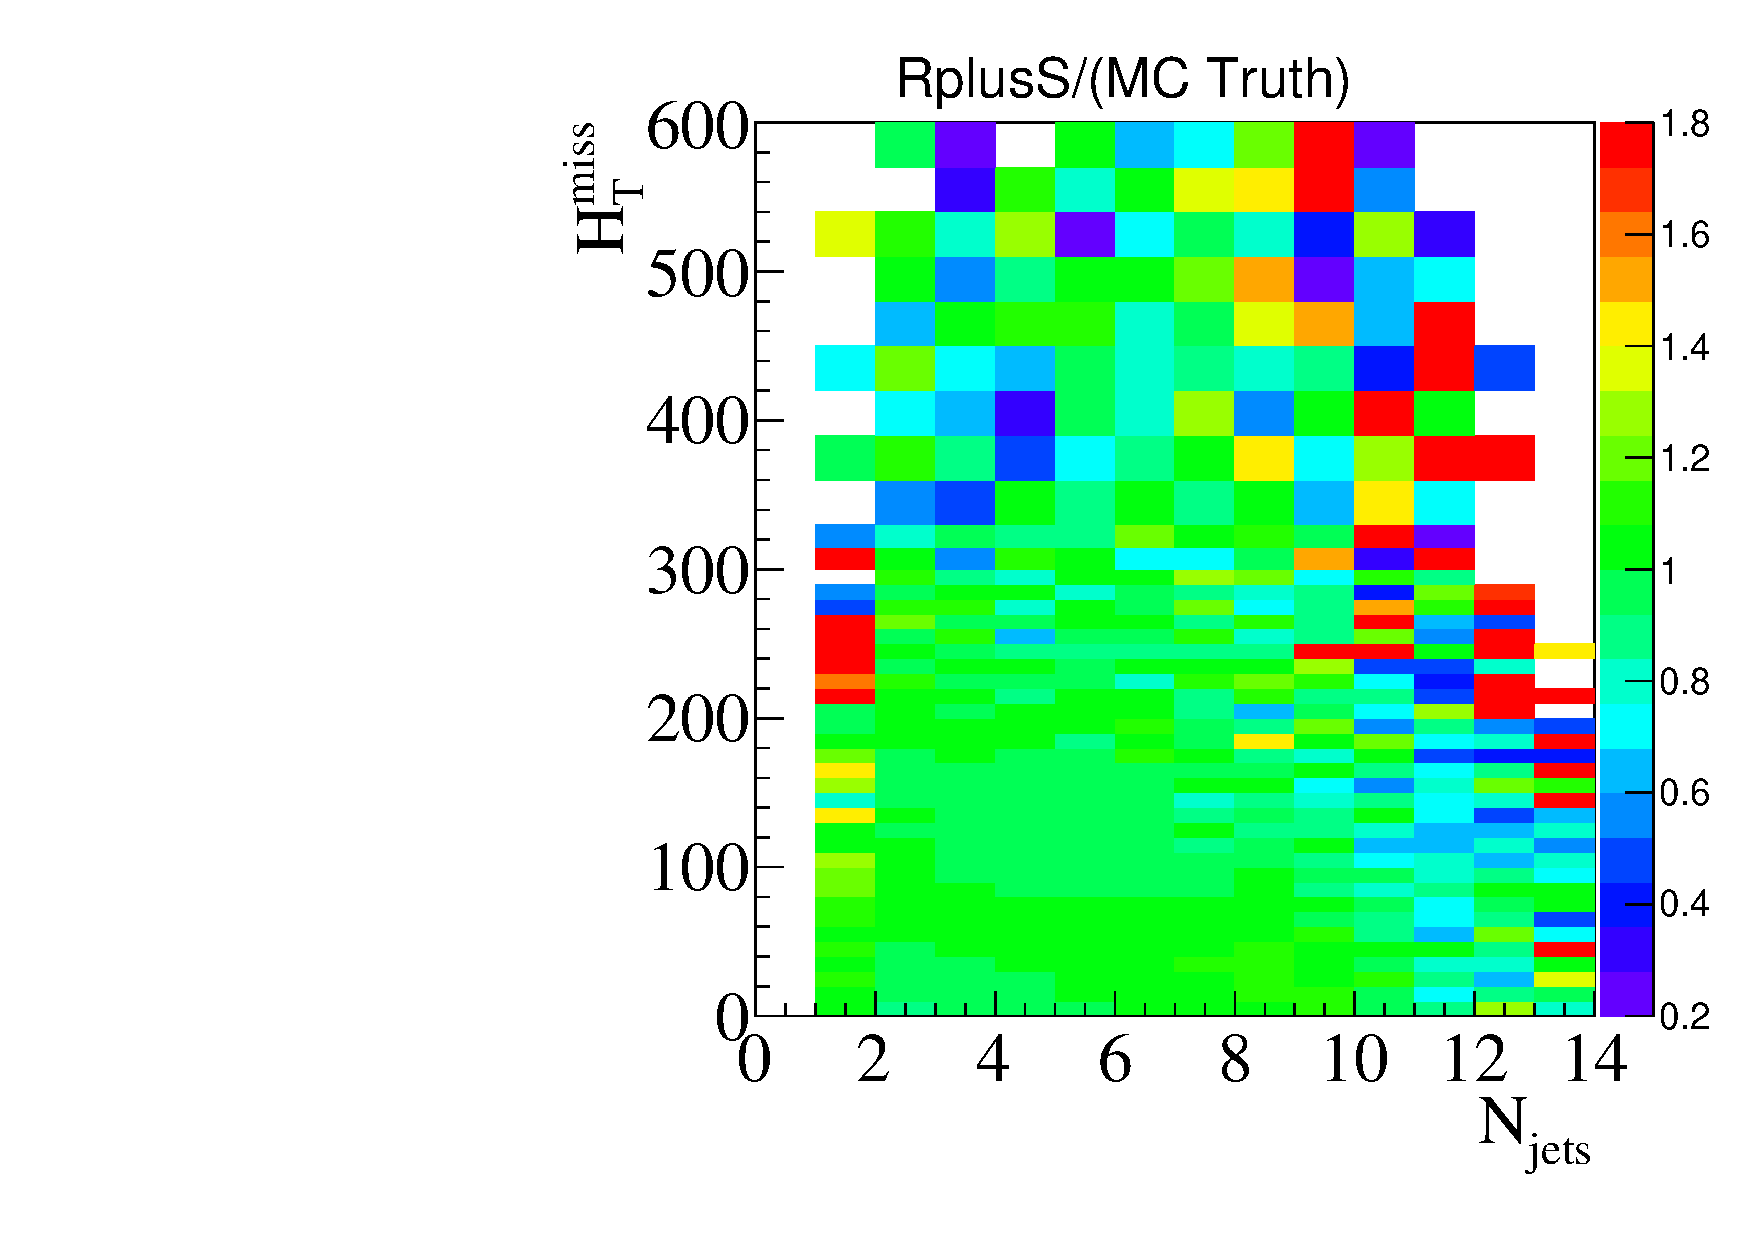
\includegraphics[width=0.5\linewidth]{figures/SusySearches/Ra2b2016/RplusSAndTruth_MhtVsNJets.pdf}
}\\
\subfloat[]{
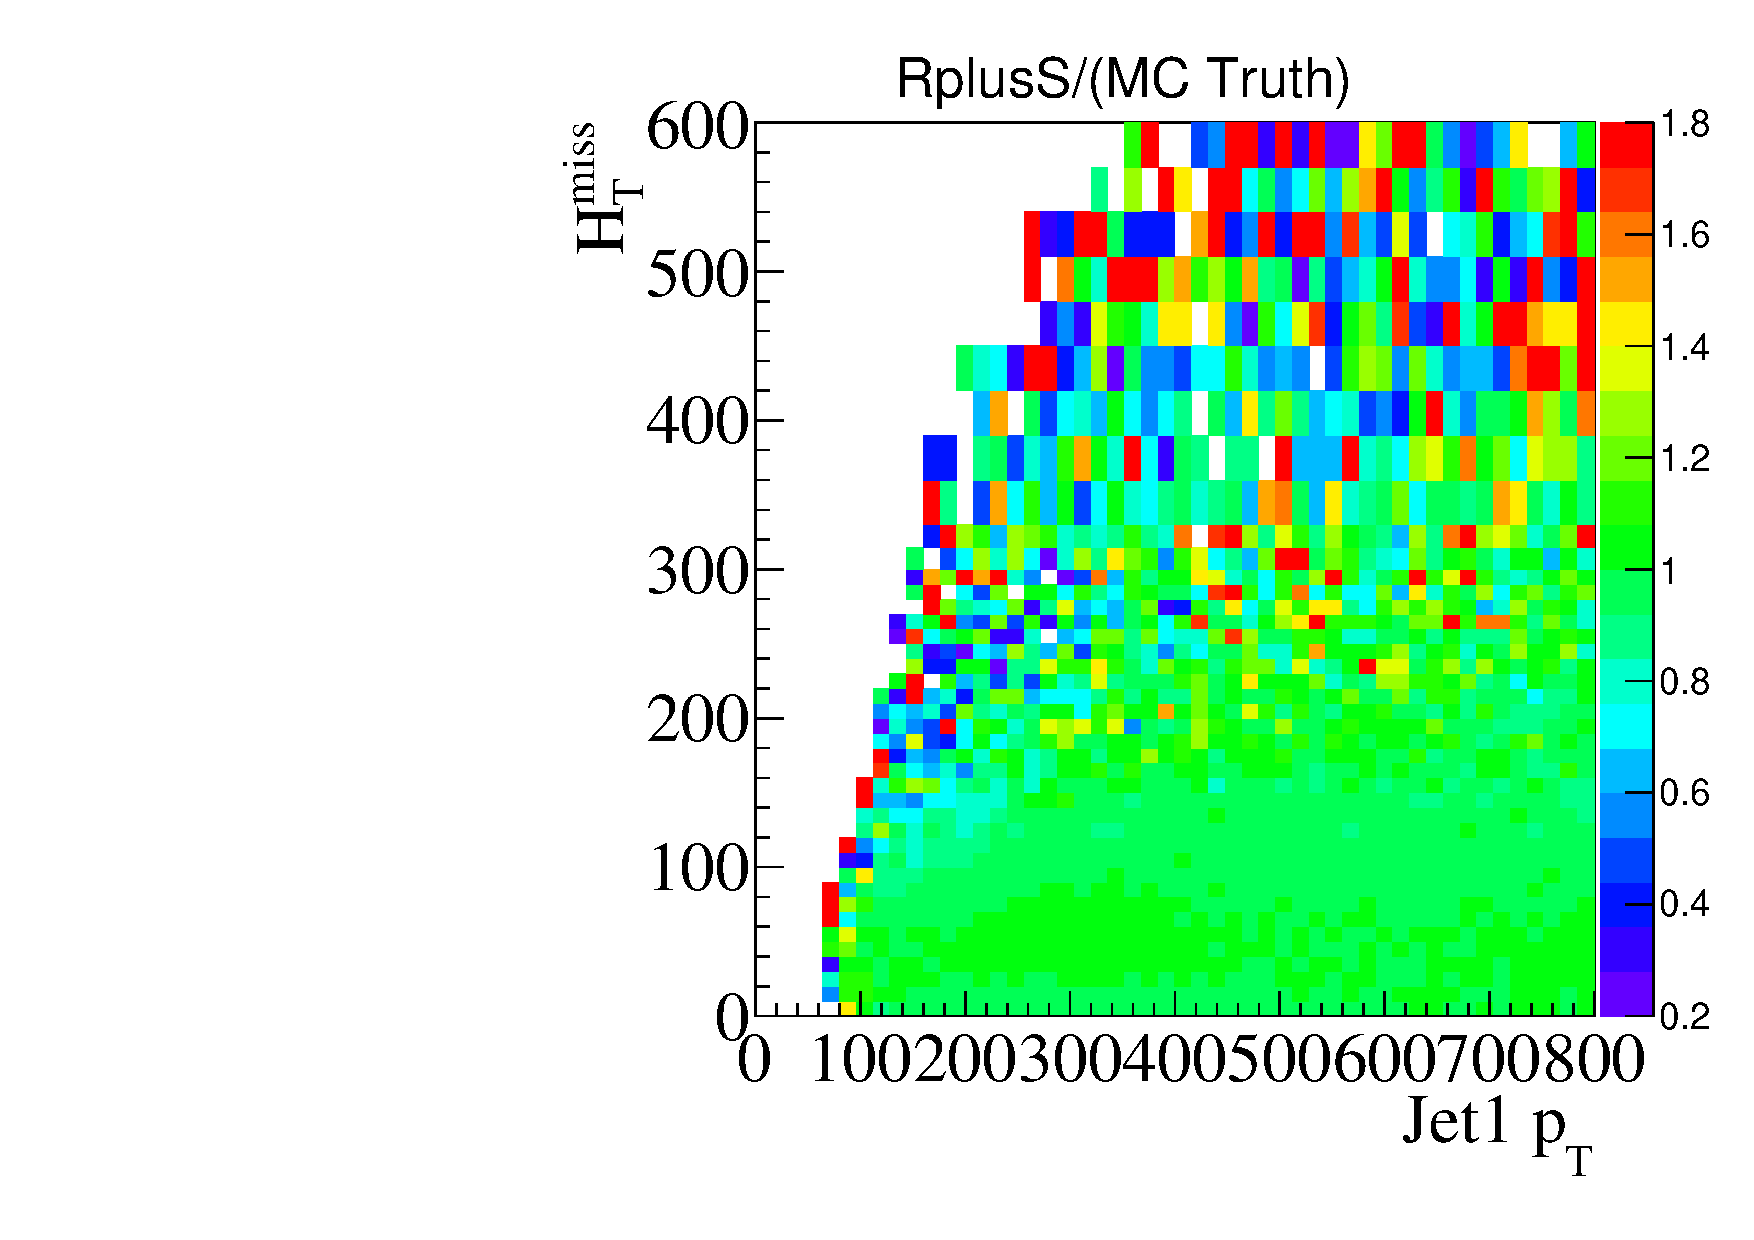
\includegraphics[width=0.5\linewidth]{figures/SusySearches/Ra2b2016/RplusSAndTruth_MhtVsJet1Pt.pdf}
}
\subfloat[]{
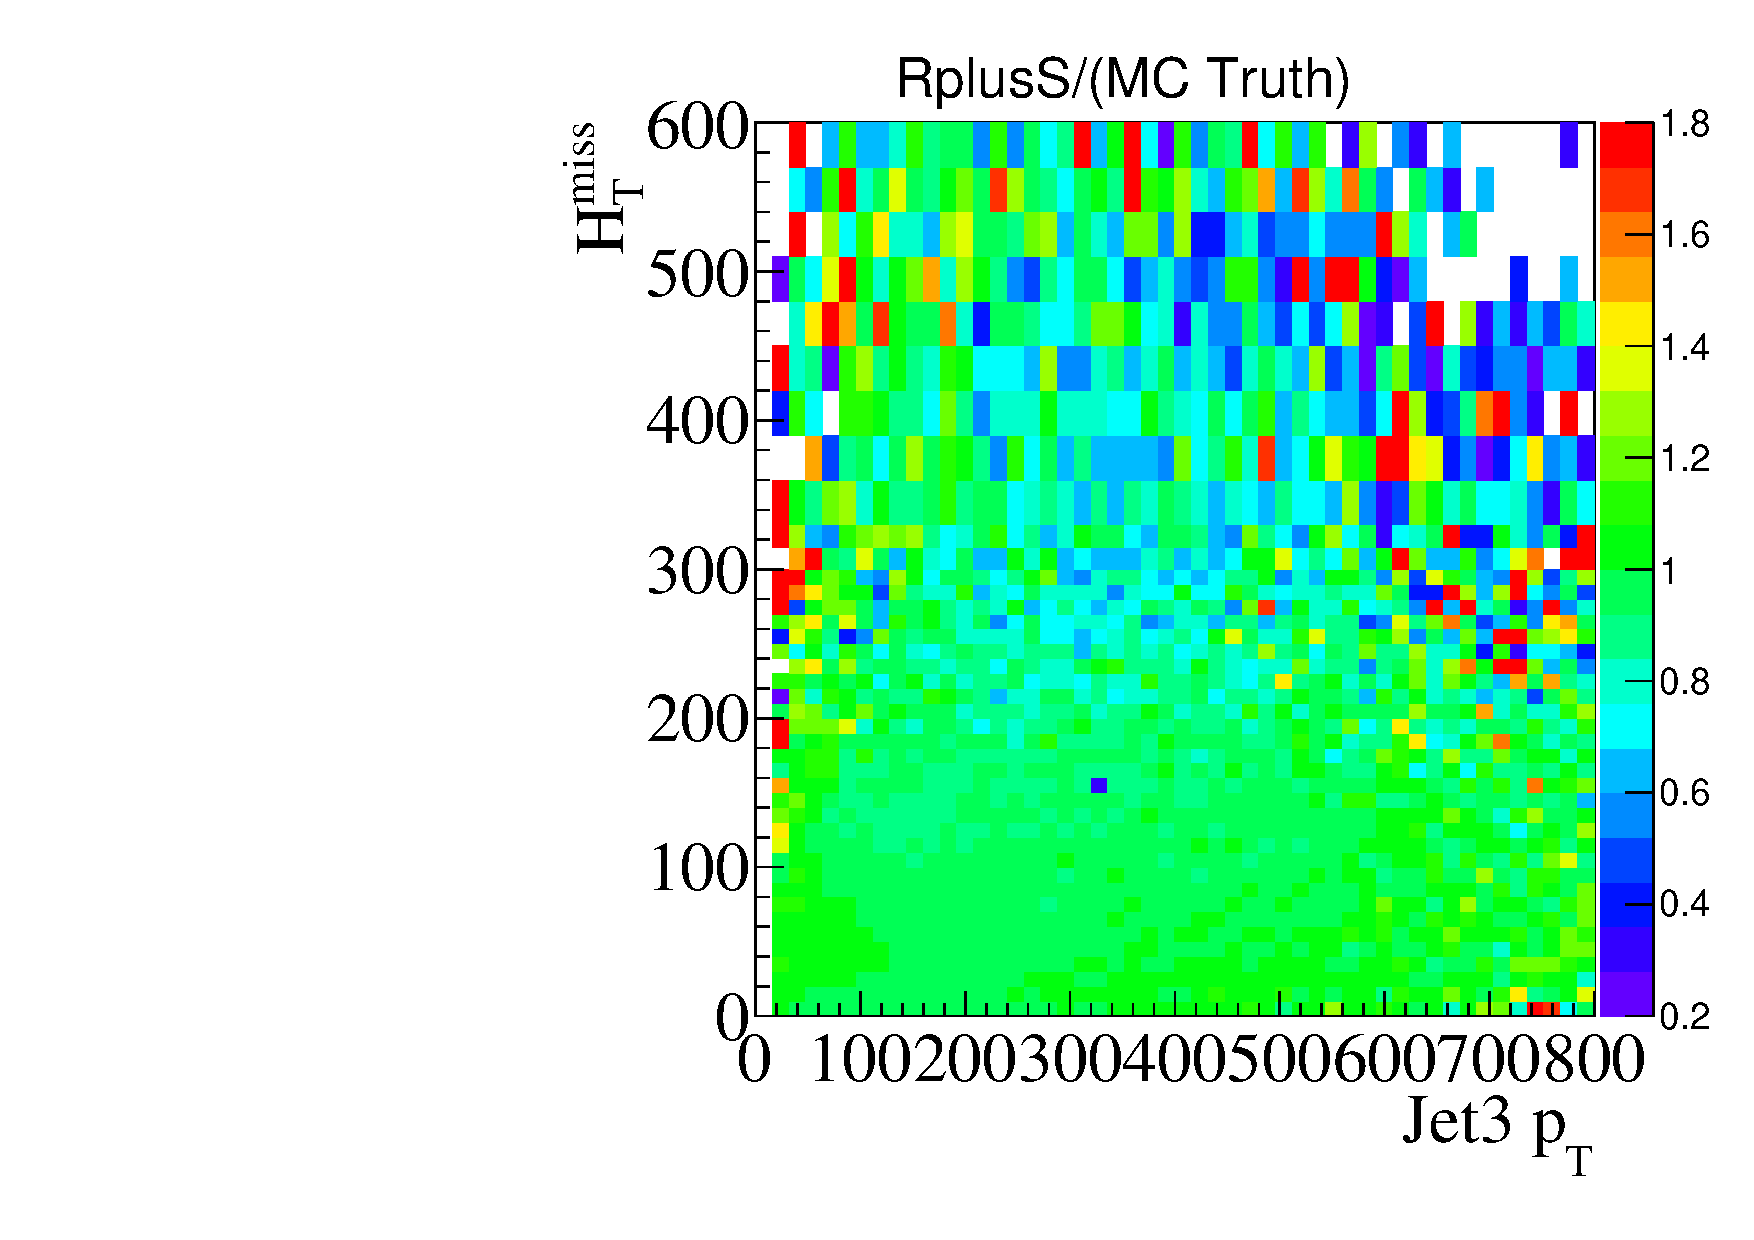
\includegraphics[width=0.5\linewidth]{figures/SusySearches/Ra2b2016/RplusSAndTruth_MhtVsJet3Pt.pdf}
}
\caption{The ratio of scatter plots of key observables for hadronic SUSY searches between the direct simulation and the rebalance and smear method applied to simulation.}
\label{fig:RplusSCorrelation}
\end{figure}
\FloatBarrier
\noindent
The degree of consistency between the prediction and the expectation in most distributions represents a significant step for QCD modeling. Not only are the relevant 1-dimensional distributions accurately modeled, but the examined pairwise correlations of the kinematic observables are accurately modeled as well. This includes correlations between the directions and magnitudes of the momenta of jets within an event, as well as relationships between the directions of the $\mht$ and the jets, and the magnitudes of the $\mht$ and $\Ht$. The most significant exception to these statements is in the distribution of the multiplicity of b-tagged jets,  where non-closure is evident for events with $\geq 3$ b-jets on the order $\approx50\%$. A possible source of this discrepancy is the choice of binning for the parton-level $\mht$ templates that constitute the prior, namely, $\nbjets=$ 0, 1, and $\geq$ 2.  A modification of this choice to include templates for the individual bins of $\nbjets=$ 2, 3, and $\geq 4$ may lead to improved results in the region of large b-jet multiplicity. 

The method is ready to be applied to the data, but the results are saved for the summary of the CMS hadronic multi-jet analysis, given in Section \ref{sec:ra2b2015}. I'll conclude now give a summary of the key developments, an try to reiterate the added value of this method.

\subsubsection{What were the key developments?}
The door has been opened for techniques that make use of correlations among jets in QCD events as a means of achieving signal-background discrimination in kinematic regions dominated by QCD, such as the regions of low-$\mht$ and low $\Ht$. Furthermore, the possibility of applying the method in the low-$\mht$ region is for the first time feasible, since the classical method did not accurately model the QCD kinematics in this region (see Fig. \ref{fig:OldVsNew}). 
\begin{figure}[h]
\centering
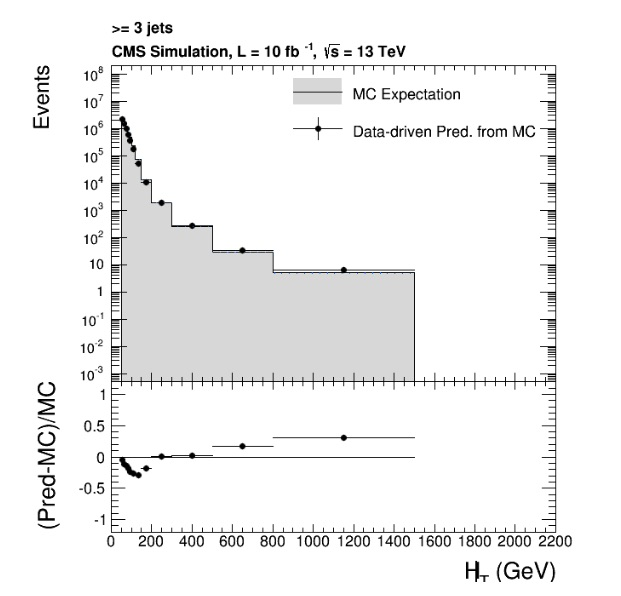
\includegraphics[width=0.49\linewidth]{figures/SusySearches/Ra2b2016/RnSClassicMht.jpg}
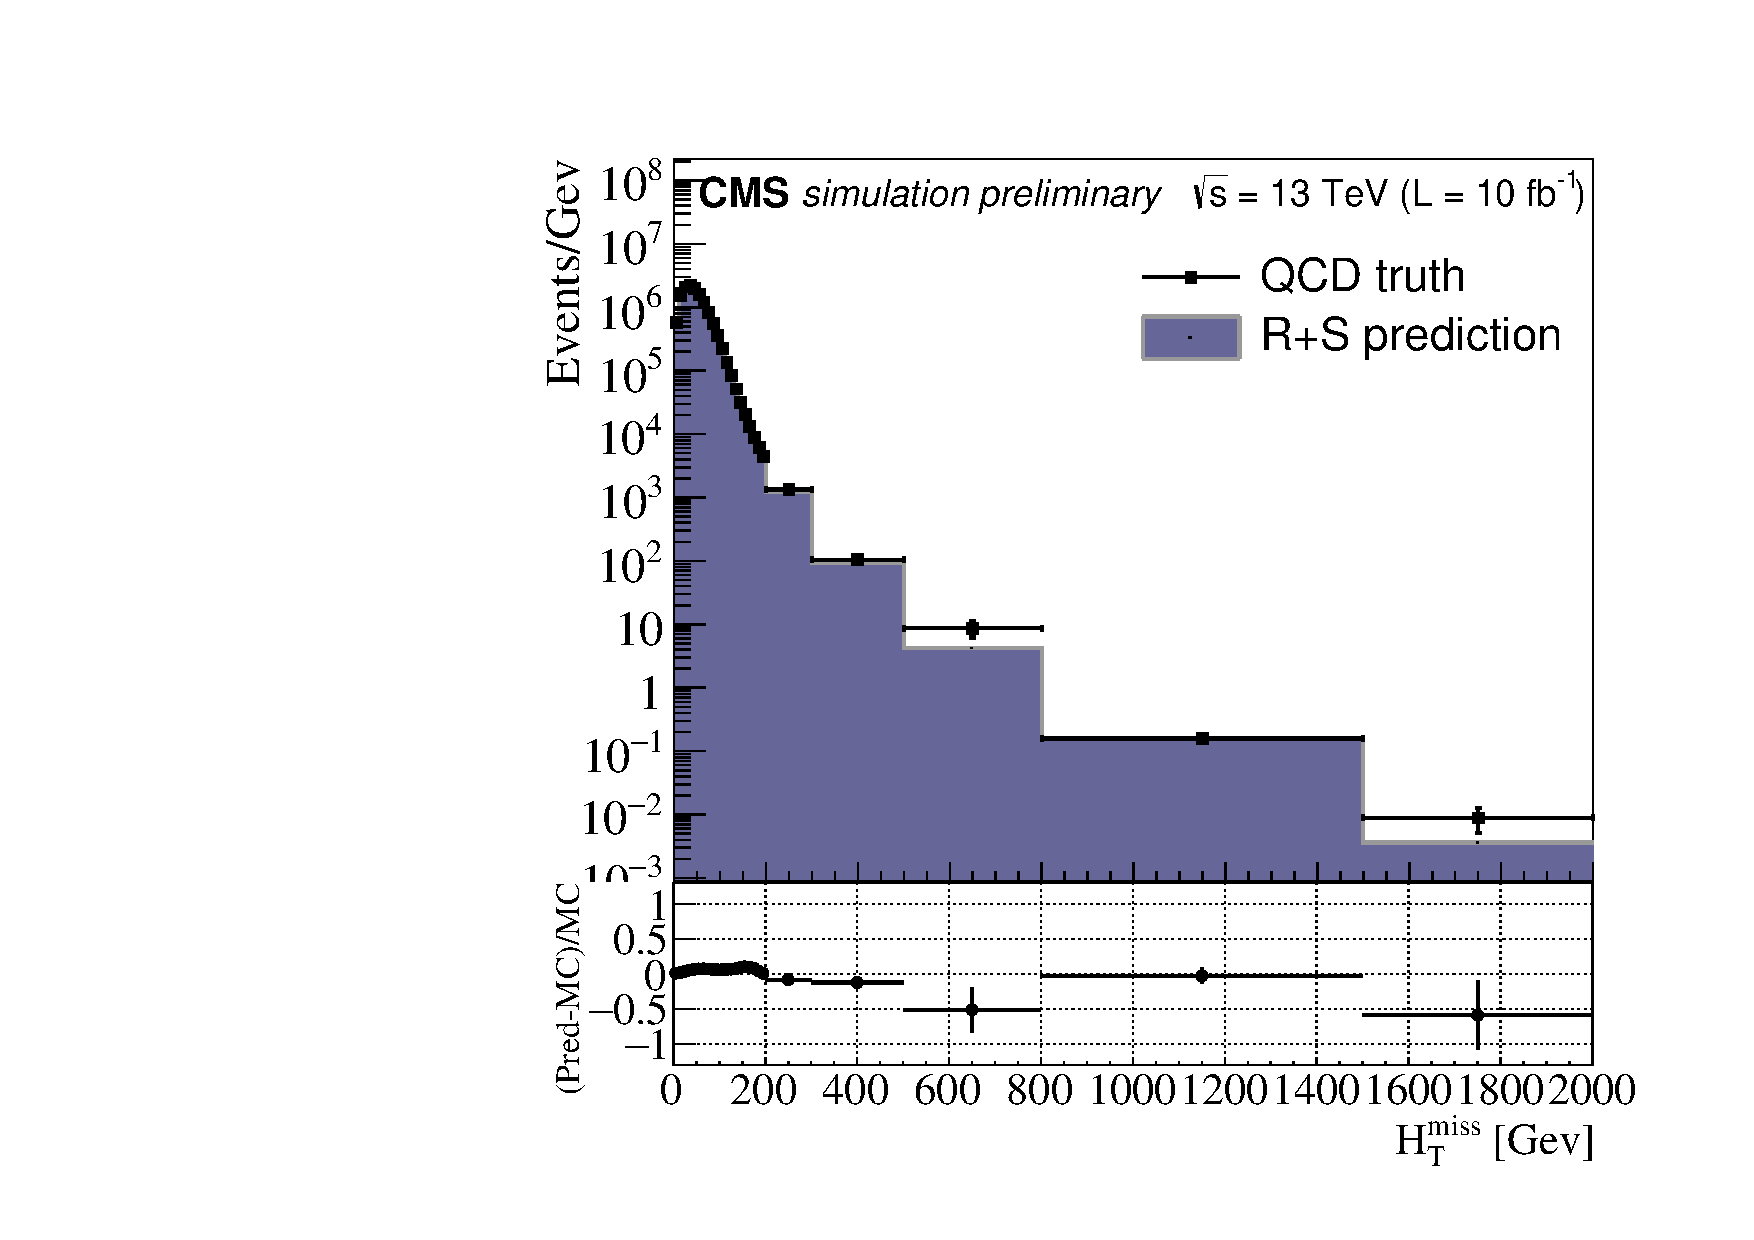
\includegraphics[width=0.49\linewidth]{figures/SusySearches/Ra2b2016/LowDeltaPhi_MhtForComparison.pdf}
\caption{Comparisons of the $\mht$ distribution between prediction and expectation using the classical method (left) and the new method (right).}
\label{fig:OldVsNew}
\end{figure}
The primary reasons for these improvements with respect to the classical method are that a realistic parton-level $\mht$ constraint is used in the rebalance procedure, whereas, in the classical method, every event is rebalanced to an $\mht$ of 0 or a constant value chosen by the user, amounting to a delta function constraint. Second, the full jet response has been used in the likelihood maximization, rather than gaussian approximations. This effect can lead to mis-modeling of the jet $\pt$ or $\mht$ spectrum in events containing jets with small $\pt$, which exhibit a highly non-Gaussian response. 

It is worth pointing out that there are two main strengths of the rebalance and smear method. The first is that it is robust against contamination from signal events in the prediction sample. The reason is that the rebalance procedure displaces signal-like, high-$\met$ events from the high-$\met$ region, to regions of low-$\met$; after smearing, the proportion of events in the high-$\met$ region truly originating from QCD processes is nearly 100\% (see Fig. \ref{fig:RplusSContamination}). 
\begin{figure}[t]
\centering
\includegraphics[width=0.6\linewidth]{figures/SusySearches/Ra2b2016/RplusSContam.pdf}
\caption{Signal contaimination removal. The midnight blue (and yellow) histograms show the distribution of QCD (and signal) events taken directly from simulation. The black (and red) histograms show the distributions of QCD (and signal) and after being processed by the rebalance and smear procedure. The signal has been removed from the high-$\mht$ region, leaving an accurately modeled QCD contribution.}
\label{fig:RplusSContamination}
\end{figure}
The robustness of the prediction to possible signal contamination in the control region allows for real events to be used directly for the prediction. The second strength is that the rebalanced events can be smeared an indefinite number of times, which allows for the accumulation of an indefinitely large prediction sample, computer resources permitting. Therefore, good estimates of the expected QCD event count and uncertainty can be made in extreme tails, even in regions for which no simulated QCD events are available. Alternatively, the rebalanced events can be smeared once to generate a training sample of background events for a multivariate discriminant, and subsequently smeared again to generate a statistically-independent prediction sample. Essentially, we have a QCD event generator, based on the data. 
\FloatBarrier
